
\documentclass[a4paper,english, UKenglish,cleveref, autoref, thm-restate]{lipics-v2021}
%This is a template for producing LIPIcs articles. 
%See lipics-v2021-authors-guidelines.pdf for further information.
%for A4 paper format use option "a4paper", for US-letter use option "letterpaper"
%for british hyphenation rules use option "UKenglish", for american hyphenation rules use option "USenglish"
%for section-numbered lemmas etc., use "numberwithinsect"
%for enabling cleveref support, use "cleveref"
%for enabling autoref support, use "autoref"
%for anonymousing the authors (e.g. for double-blind review), add "anonymous"
%for enabling thm-restate support, use "thm-restate"
%for enabling a two-column layout for the author/affilation part (only applicable for > 6 authors), use "authorcolumns"
%for producing a PDF according the PDF/A standard, add "pdfa"

%\pdfoutput=1 %uncomment to ensure pdflatex processing (mandatatory e.g. to submit to arXiv)
%\hideLIPIcs  %uncomment to remove references to LIPIcs series (logo, DOI, ...), e.g. when preparing a pre-final version to be uploaded to arXiv or another public repository

%\graphicspath{{./graphics/}}%helpful if your graphic files are in another directory

\usepackage{cite}
\usepackage{amsmath,amssymb,amsfonts}
\usepackage{algorithmic}
\usepackage{graphicx}
\usepackage{bussproofs}
\EnableBpAbbreviations
\usepackage{hyperref}
\usepackage{tikz,pgfplots}
\pgfplotsset{compat=newest}
\usepackage{tikz-cd}
\usepackage{textcomp}
\usepackage{xcolor}
\usepackage{amsthm}
\usepackage{caption}
\usepackage{subcaption}
\usetikzlibrary{cd}
\usepackage{mathabx}
\usepackage{cmll}
\usepackage{stmaryrd}
\usepackage{wrapfig}
\usepackage{relsize}

\usetikzlibrary{intersections,through}

\message{<Paul Taylor's Proof Trees, 2 August 1996>}
%% Build proof tree for Natural Deduction, Sequent Calculus, etc.
%% WITH SHORTENING OF PROOF RULES!
%% Paul Taylor, begun 10 Oct 1989
%% *** THIS IS ONLY A PRELIMINARY VERSION AND THINGS MAY CHANGE! ***
%%
%% 2 Aug 1996: fixed \mscount and \proofdotnumber
%%
%%      \prooftree
%%              hyp1            produces:
%%              hyp2
%%              hyp3            hyp1    hyp2    hyp3
%%      \justifies              -------------------- rulename
%%              concl                   concl
%%      \thickness=0.08em
%%      \shiftright 2em
%%      \using
%%              rulename
%%      \endprooftree
%%
%% where the hypotheses may be similar structures or just formulae.
%%
%% To get a vertical string of dots instead of the proof rule, do
%%
%%      \prooftree                      which produces:
%%              [hyp]
%%      \using                                  [hyp]
%%              name                              .
%%      \proofdotseparation=1.2ex                 .name
%%      \proofdotnumber=4                         .
%%      \leadsto                                  .
%%              concl                           concl
%%      \endprooftree
%%
%% Within a prooftree, \[ and \] may be used instead of \prooftree and
%% \endprooftree; this is not permitted at the outer level because it
%% conflicts with LaTeX. Also,
%%      \Justifies
%% produces a double line. In LaTeX you can use \begin{prooftree} and
%% \end{prootree} at the outer level (however this will not work for the inner
%% levels, but in any case why would you want to be so verbose?).
%%
%% All of of the keywords except \prooftree and \endprooftree are optional
%% and may appear in any order. They may also be combined in \newcommand's
%% eg "\def\Cut{\using\sf cut\thickness.08em\justifies}" with the abbreviation
%% "\prooftree hyp1 hyp2 \Cut \concl \endprooftree". This is recommended and
%% some standard abbreviations will be found at the end of this file.
%%
%% \thickness specifies the breadth of the rule in any units, although
%% font-relative units such as "ex" or "em" are preferable.
%% It may optionally be followed by "=".
%% \proofrulebreadth=.08em or \setlength\proofrulebreadth{.08em} may also be
%% used either in place of \thickness or globally; the default is 0.04em.
%% \proofdotseparation and \proofdotnumber control the size of the
%% string of dots
%%
%% If proof trees and formulae are mixed, some explicit spacing is needed,
%% but don't put anything to the left of the left-most (or the right of
%% the right-most) hypothesis, or put it in braces, because this will cause
%% the indentation to be lost.
%%
%% By default the conclusion is centered wrt the left-most and right-most
%% immediate hypotheses (not their proofs); \shiftright or \shiftleft moves
%% it relative to this position. (Not sure about this specification or how
%% it should affect spreading of proof tree.)
%
% global assignments to dimensions seem to have the effect of stretching
% diagrams horizontally.
%
%%==========================================================================

\def\introrule{{\cal I}}\def\elimrule{{\cal E}}%%
\def\andintro{\using{\land}\introrule\justifies}%%
\def\impelim{\using{\Rightarrow}\elimrule\justifies}%%
\def\allintro{\using{\forall}\introrule\justifies}%%
\def\allelim{\using{\forall}\elimrule\justifies}%%
\def\falseelim{\using{\bot}\elimrule\justifies}%%
\def\existsintro{\using{\exists}\introrule\justifies}%%

%% #1 is meant to be 1 or 2 for the first or second formula
\def\andelim#1{\using{\land}#1\elimrule\justifies}%%
\def\orintro#1{\using{\lor}#1\introrule\justifies}%%

%% #1 is meant to be a label corresponding to the discharged hypothesis/es
\def\impintro#1{\using{\Rightarrow}\introrule_{#1}\justifies}%%
\def\orelim#1{\using{\lor}\elimrule_{#1}\justifies}%%
\def\existselim#1{\using{\exists}\elimrule_{#1}\justifies}

%%==========================================================================

\newdimen\proofrulebreadth \proofrulebreadth=.05em
\newdimen\proofdotseparation \proofdotseparation=1.25ex
\newdimen\proofrulebaseline \proofrulebaseline=2ex
\newcount\proofdotnumber \proofdotnumber=3
\let\then\relax
\def\hfi{\hskip0pt plus.0001fil}
\mathchardef\squigto="3A3B
%
% flag where we are
\newif\ifinsideprooftree\insideprooftreefalse
\newif\ifonleftofproofrule\onleftofproofrulefalse
\newif\ifproofdots\proofdotsfalse
\newif\ifdoubleproof\doubleprooffalse
\let\wereinproofbit\relax
%
% dimensions and boxes of bits
\newdimen\shortenproofleft
\newdimen\shortenproofright
\newdimen\proofbelowshift
\newbox\proofabove
\newbox\proofbelow
\newbox\proofrulename
%
% miscellaneous commands for setting values
\def\shiftproofbelow{\let\next\relax\afterassignment\setshiftproofbelow\dimen0 }
\def\shiftproofbelowneg{\def\next{\multiply\dimen0 by-1 }%
\afterassignment\setshiftproofbelow\dimen0 }
\def\setshiftproofbelow{\next\proofbelowshift=\dimen0 }
\def\setproofrulebreadth{\proofrulebreadth}

%=============================================================================
\def\prooftree{% NESTED ZERO (\ifonleftofproofrule)
%
% first find out whether we're at the left-hand end of a proof rule
\ifnum  \lastpenalty=1
\then   \unpenalty
\else   \onleftofproofrulefalse
\fi
%
% some space on left (except if we're on left, and no infinity for outermost)
\ifonleftofproofrule
\else   \ifinsideprooftree
        \then   \hskip.5em plus1fil
        \fi
\fi
%
% begin our proof tree environment
\bgroup% NESTED ONE (\proofbelow, \proofrulename, \proofabove,
%               \shortenproofleft, \shortenproofright, \proofrulebreadth)
\setbox\proofbelow=\hbox{}\setbox\proofrulename=\hbox{}%
\let\justifies\proofover\let\leadsto\proofoverdots\let\Justifies\proofoverdbl
\let\using\proofusing\let\[\prooftree
\ifinsideprooftree\let\]\endprooftree\fi
\proofdotsfalse\doubleprooffalse
\let\thickness\setproofrulebreadth
\let\shiftright\shiftproofbelow \let\shift\shiftproofbelow
\let\shiftleft\shiftproofbelowneg
\let\ifwasinsideprooftree\ifinsideprooftree
\insideprooftreetrue
%
% now begin to set the top of the rule (definitions local to it)
\setbox\proofabove=\hbox\bgroup$\displaystyle % NESTED TWO
\let\wereinproofbit\prooftree
%
% these local variables will be copied out:
\shortenproofleft=0pt \shortenproofright=0pt \proofbelowshift=0pt
%
% flags to enable inner proof tree to detect if on left:
\onleftofproofruletrue\penalty1
}

%=============================================================================
% end whatever box and copy crucial values out of it
\def\eproofbit{% NESTED TWO
%
% various hacks applicable to hypothesis list 
\ifx    \wereinproofbit\prooftree
\then   \ifcase \lastpenalty
        \then   \shortenproofright=0pt  % 0: some other object, no indentation
        \or     \unpenalty\hfil         % 1: empty hypotheses, just glue
        \or     \unpenalty\unskip       % 2: just had a tree, remove glue
        \else   \shortenproofright=0pt  % eh?
        \fi
\fi
%
% pass out crucial values from scope
\global\dimen0=\shortenproofleft
\global\dimen1=\shortenproofright
\global\dimen2=\proofrulebreadth
\global\dimen3=\proofbelowshift
\global\dimen4=\proofdotseparation
\global\count255=\proofdotnumber
%
% end the box
$\egroup  % NESTED ONE
%
% restore the values
\shortenproofleft=\dimen0
\shortenproofright=\dimen1
\proofrulebreadth=\dimen2
\proofbelowshift=\dimen3
\proofdotseparation=\dimen4
\proofdotnumber=\count255
}

%=============================================================================
\def\proofover{% NESTED TWO
\eproofbit % NESTED ONE
\setbox\proofbelow=\hbox\bgroup % NESTED TWO
\let\wereinproofbit\proofover
$\displaystyle
}%
%
%=============================================================================
\def\proofoverdbl{% NESTED TWO
\eproofbit % NESTED ONE
\doubleprooftrue
\setbox\proofbelow=\hbox\bgroup % NESTED TWO
\let\wereinproofbit\proofoverdbl
$\displaystyle
}%
%
%=============================================================================
\def\proofoverdots{% NESTED TWO
\eproofbit % NESTED ONE
\proofdotstrue
\setbox\proofbelow=\hbox\bgroup % NESTED TWO
\let\wereinproofbit\proofoverdots
$\displaystyle
}%
%
%=============================================================================
\def\proofusing{% NESTED TWO
\eproofbit % NESTED ONE
\setbox\proofrulename=\hbox\bgroup % NESTED TWO
\let\wereinproofbit\proofusing
\kern0.3em$
}

%=============================================================================
\def\endprooftree{% NESTED TWO
\eproofbit % NESTED ONE
% \dimen0 =     length of proof rule
% \dimen1 =     indentation of conclusion wrt rule
% \dimen2 =     new \shortenproofleft, ie indentation of conclusion
% \dimen3 =     new \shortenproofright, ie
%                space on right of conclusion to end of tree
% \dimen4 =     space on right of conclusion below rule
  \dimen5 =0pt% spread of hypotheses
% \dimen6, \dimen7 = height & depth of rule
%
% length of rule needed by proof above
\dimen0=\wd\proofabove \advance\dimen0-\shortenproofleft
\advance\dimen0-\shortenproofright
%
% amount of spare space below
\dimen1=.5\dimen0 \advance\dimen1-.5\wd\proofbelow
\dimen4=\dimen1
\advance\dimen1\proofbelowshift \advance\dimen4-\proofbelowshift
%
% conclusion sticks out to left of immediate hypotheses
\ifdim  \dimen1<0pt
\then   \advance\shortenproofleft\dimen1
        \advance\dimen0-\dimen1
        \dimen1=0pt
%       now it sticks out to left of tree!
        \ifdim  \shortenproofleft<0pt
        \then   \setbox\proofabove=\hbox{%
                        \kern-\shortenproofleft\unhbox\proofabove}%
                \shortenproofleft=0pt
        \fi
\fi
%
% and to the right
\ifdim  \dimen4<0pt
\then   \advance\shortenproofright\dimen4
        \advance\dimen0-\dimen4
        \dimen4=0pt
\fi
%
% make sure enough space for label
\ifdim  \shortenproofright<\wd\proofrulename
\then   \shortenproofright=\wd\proofrulename
\fi
%
% calculate new indentations
\dimen2=\shortenproofleft \advance\dimen2 by\dimen1
\dimen3=\shortenproofright\advance\dimen3 by\dimen4
%
% make the rule or dots, with name attached
\ifproofdots
\then
        \dimen6=\shortenproofleft \advance\dimen6 .5\dimen0
        \setbox1=\vbox to\proofdotseparation{\vss\hbox{$\cdot$}\vss}%
        \setbox0=\hbox{%
                \advance\dimen6-.5\wd1
                \kern\dimen6
                $\vcenter to\proofdotnumber\proofdotseparation
                        {\leaders\box1\vfill}$%
                \unhbox\proofrulename}%
\else   \dimen6=\fontdimen22\the\textfont2 % height of maths axis
        \dimen7=\dimen6
        \advance\dimen6by.5\proofrulebreadth
        \advance\dimen7by-.5\proofrulebreadth
        \setbox0=\hbox{%
                \kern\shortenproofleft
                \ifdoubleproof
                \then   \hbox to\dimen0{%
                        $\mathsurround0pt\mathord=\mkern-6mu%
                        \cleaders\hbox{$\mkern-2mu=\mkern-2mu$}\hfill
                        \mkern-6mu\mathord=$}%
                \else   \vrule height\dimen6 depth-\dimen7 width\dimen0
                \fi
                \unhbox\proofrulename}%
        \ht0=\dimen6 \dp0=-\dimen7
\fi
%
% set up to centre outermost tree only
\let\doll\relax
\ifwasinsideprooftree
\then   \let\VBOX\vbox
\else   \ifmmode\else$\let\doll=$\fi
        \let\VBOX\vcenter
\fi
% this \vbox or \vcenter is the actual output:
\VBOX   {\baselineskip\proofrulebaseline \lineskip.2ex
        \expandafter\lineskiplimit\ifproofdots0ex\else-0.6ex\fi
        \hbox   spread\dimen5   {\hfi\unhbox\proofabove\hfi}%
        \hbox{\box0}%
        \hbox   {\kern\dimen2 \box\proofbelow}}\doll%
%
% pass new indentations out of scope
\global\dimen2=\dimen2
\global\dimen3=\dimen3
\egroup % NESTED ZERO
\ifonleftofproofrule
\then   \shortenproofleft=\dimen2
\fi
\shortenproofright=\dimen3
%
% some space on right and flag we've just made a tree
\onleftofproofrulefalse
\ifinsideprooftree
\then   \hskip.5em plus 1fil \penalty2
\fi
}

%==========================================================================
% IDEAS
% 1.    Specification of \shiftright and how to spread trees.
% 2.    Spacing command \m which causes 1em+1fil spacing, over-riding
%       exisiting space on sides of trees and not affecting the
%       detection of being on the left or right.
% 3.    Hack using \@currenvir to detect LaTeX environment; have to
%       use \aftergroup to pass \shortenproofleft/right out.
% 4.    (Pie in the sky) detect how much trees can be "tucked in"
% 5.    Discharged hypotheses (diagonal lines).

\usepackage{proof}

\bibliographystyle{plainurl}% the mandatory bibstyle



% MATH TEXT STYLES
\newcommand{\B}[1]{\mathbf{#1}}
\newcommand{\BB}[1]{\mathbb{#1}}
\newcommand{\C}[1]{\mathcal{#1}}
\newcommand{\F}[1]{\mathfrak{#1}}
\newcommand{\TT}[1]{\mathtt{#1}}
\newcommand{\RM}[1]{\mathrm{#1}}
\newcommand{\SF}[1]{\mathsf{#1}}



%CATEGORIES

\newcommand{\Met}{\mathsf{Met}}
\newcommand{\Mod}{\Lawv\mathsf{Mod}}
\newcommand{\GMet}{\Lawv\mathsf{CCat}}
\newcommand{\Fun}{\mathsf{Fun}}
\newcommand{\colim}{\mathrm{colim}}
\newcommand{\Yon}{\B{Y}}
\newcommand{\Hom}{\mathrm{Hom}}
\newcommand{\Sym}{\mathrm{Sym}}
\newcommand{\matr}[1]{\hat{#1}}

\newcommand\pfun{\mathrel{\ooalign{\hfil$\mapstochar\mkern5mu$\hfil\cr$\to$\cr}}}



% LAMBDA CALCULI

\newcommand{\lamcalc}{$\lambda$-calculus}
\newcommand{\lam}{\lambda}

\newcommand{\STLC}{\RM{STLC}}
\newcommand{\BSTLC}{\mathsf b\RM{STLC}}
\newcommand{\RSTLC}{\C R\RM{STLC}}
\newcommand{\STDLC}{\RM{ST}\partial\RM{LC}}
\newcommand{\Real}{\SF{Real}}

\newcommand{\Der}{\SF D}
\newcommand{\To}{\Rightarrow}
\newcommand{\Diff}[2]{\Der[#1,#2]}

\newcommand{\finMS}[1]{\C M_{\RM{fin}}(#1)}

\newcommand{\true}{\prog{True}}
\newcommand{\false}{\prog{False}}
\newcommand{\bool}{\SF{Bool}}

\newcommand{\Te}[1]{\C T(#1)}

\newcommand{\prog}[1]{\mathtt{#1}}




% METRIC STUFF
\newcommand{\Lawv}{\BB L}
\newcommand{\QualREL}[1]{#1 \SF{Rel}}
\newcommand{\QREL}{\QualREL{Q}}
\newcommand{\LREL}{\QualREL{\Lawv}}
\newcommand{\LCAT}{\Lawv\SF{CCat}}

\newcommand{\op}{\mathrm{op}} 
\newcommand{\sk}{\mathrm{sk}} 
\newcommand{\sym}{\mathrm{sym}} 
\newcommand{\menus}{\dotdiv} 

\newcommand{\norm}[1]{\lVert#1\rVert}
\newcommand{\supnorm}[1]{\lVert#1\rVert_\infty}
\newcommand{\absv}[1]{\left\lvert#1\right\rvert}

% TROPICAL STUFF

\newcommand{\trop}[1]{\SF t #1}
\newcommand{\model}[1]{\llbracket#1\rrbracket}
\newcommand{\nodel}[1]{\langle #1\rangle}
\newcommand{\sumt}[1]{{+}^{#1}}
\newcommand{\prodt}[1]{{\times}^{#1}}


% MISCELLANEOUS

\newcommand{\HOM}[3]{{#1}(#2,#3)}
\newcommand{\N}{\BB N}
\newcommand{\R}{\BB R}
\newcommand{\set}[1]{\{#1\}}
\newcommand{\multiset}{\C M_{\mathrm{fin}}}

\newcommand{\eps}{\epsilon}

\newcommand{\twoheaddownarrow}{\mathrel{\rotatebox[origin=c]{270}{$\twoheadrightarrow$}}\!}


%LIST ENVIRONMENTS


\newenvironment{varenumerate}
{
	\begin{list}{\arabic{numberone}.}
		{
			\usecounter{numberone}
			\setlength{\itemsep}{0pt}
			\setlength{\topsep}{0pt}
			\setlength{\parsep}{0pt}
			\setlength{\partopsep}{0pt}
			\setlength{\leftmargin}{15pt}
			\setlength{\rightmargin}{0pt}
			\setlength{\itemindent}{0pt}
			\setlength{\labelsep}{5pt}
			\setlength{\labelwidth}{15pt}
	}}
	{
	\end{list} 
}





%MATH EVIRONMENTS











\title{Tropical mathematics and the Lambda-calculus I}
\subtitle{Metric and Differential Analysis of Effectful Programs
} %TODO Please add

\titlerunning{Tropical mathematics for the Lambda-calculus 1} %TODO optional, please use if title is longer than one line

\author{Davide {Barbarossa}}{Dipartimento di Informatica - Scienza e Ingegneria, Universit\`a di Bologna, %[optional: Address], 
Italy% \and My second affiliation, Country 
\and \url{https://lipn.univ-paris13.fr/\~barbarossa/index.html} }{davide.barbarossa@unibo.it}{https://orcid.org/0000-0003-4608-8282}{%(Optional)Funding each author
}%TODO mandatory, please use full name; only 1 author per \author macro; first two parameters are mandatory, other parameters can be empty. Please provide at least the name of the affiliation and the country. The full address is optional. Use additional curly braces to indicate the correct name splitting when the last name consists of multiple name parts.

\author{Paolo {Pistone}}{Dipartimento di Informatica - Scienza e Ingegneria, Universit\`a di Bologna, %[optional: Address], 
Italy% \and LIP, Universit\'e de Lyon, France 
\and \url{http://logica.uniroma3.it/pistone/
} }{paolo.pistone2@unibo.it}{https://orcid.org/0000-0003-4250-9051}{%(Optional)Funding each author
}


\authorrunning{D.\,Barbarossa and P.\,Pistone} %TODO mandatory. First: Use abbreviated first/middle names. Second (only in severe cases): Use first author plus 'et al.'

\Copyright{Davide Barbarossa and Paolo Pistone} %TODO mandatory, please use full first names. LIPIcs license is "CC-BY";  http://creativecommons.org/licenses/by/3.0/

\ccsdesc[500]{Theory of computation~Lambda calculus}
\ccsdesc[300]{Theory of computation~Categorical semantics}
\ccsdesc[100]{Theory of computation~Linear logic}%TODO mandatory: Please choose ACM 2012 classifications from https://dl.acm.org/ccs/ccs_flat.cfm 

\keywords{Relational semantics, Differential lambda-calculus, Tropical semiring,  Program metrics, Lawvere quantale} %TODO mandatory; please add comma-separated list of keywords

\category{} %optional, e.g. invited paper

\relatedversion{} %optional, e.g. full version hosted on arXiv, HAL, or other respository/website
%\relatedversiondetails[linktext={opt. text shown instead of the URL}, cite=DBLP:books/mk/GrayR93]{Classification (e.g. Full Version, Extended Version, Previous Version}{URL to related version} %linktext and cite are optional

%\supplement{}%optional, e.g. related research data, source code, ... hosted on a repository like zenodo, figshare, GitHub, ...
%\supplementdetails[linktext={opt. text shown instead of the URL}, cite=DBLP:books/mk/GrayR93, subcategory={Description, Subcategory}, swhid={Software Heritage Identifier}]{General Classification (e.g. Software, Dataset, Model, ...)}{URL to related version} %linktext, cite, and subcategory are optional

\funding{This work has been supported by the ERC CoG 818616 DIAPASoN.}%optional, to capture a funding statement, which applies to all authors. Please enter author specific funding statements as fifth argument of the \author macro.

\acknowledgements{%I want to thank \dots
}%optional

%\nolinenumbers %uncomment to disable line numbering



%Editor-only macros:: begin (do not touch as author)%%%%%%%%%%%%%%%%%%%%%%%%%%%%%%%%%%
\EventEditors{John Q. Open and Joan R. Access}
\EventNoEds{2}
\EventLongTitle{42nd Conference on Very Important Topics (CVIT 2016)}
\EventShortTitle{CVIT 2016}
\EventAcronym{CVIT}
\EventYear{2016}
\EventDate{December 24--27, 2016}
\EventLocation{Little Whinging, United Kingdom}
\EventLogo{}
\SeriesVolume{42}
\ArticleNo{23}
%%%%%%%%%%%%%%%%%%%%%%%%%%%%%%%%%%%%%%%%%%%%%%%%%%%%%%

\begin{document}

\maketitle

%TODO mandatory: add short abstract of the document
\begin{abstract}
We study the interpretation of the lambda-calculus in a framework based on tropical mathematics, and we show that it provides a unified framework for both program  metrics, based on the analysis of program sensitivity via Lipschitz conditions, and resource analysis, based on higher-order program differentiation. 
To do that we focus on the semantics arising from the relational model weighted over the tropical semiring, and we discuss its application to the study of “best case” program behavior for languages with probabilistic and non-deterministic effects. Finally, we show that a general foundation for this approach is provided by an abstract correspondence between tropical algebra and Lawvere’s theory of generalized metric spaces.
%A typical result of such line of research is that, thanks to the tropical operations, a simply typed term is interpreted as a locally Lipschitz map, which is in turn decomposed as an inf of more and more sensitive Lipschitz ones, corresponding to the interpretations of the approximants given by the lambda-calculus Taylor expansion.
%We finally describe some promising lines of research, showing in particular how such tropical model expresses natural optimisation problems of probabilistic calculi.
\end{abstract}

\section{Introduction}

In recent years, more and more interest in the programming language community has been directed towards the study of \emph{quantitative} properties of programs like computing the number of computation steps or convergence probabilities, 
as opposed to purely \emph{qualitative} properties like termination or program equivalence. 
Notably, a significant effort has been made to extend, or adapt, well-established qualitative methods, like type systems, relational logics or denotational semantics, to account for quantitative properties. We can mention, for example, 
intersection type systems aimed at capturing time or space resources \cite{decarvalho2018, Accattoli2022} or convergence probabilities \cite{Breuvart2018, PistoneLICS2022},  relational logics to account for probabilistic properties like e.g.~differential privacy \cite{Barthe_2012} or metric preservation \cite{Reed2010, dallago}, as well as the study of denotational models for 
probabilistic \cite{Ehrhard2011, Staton2017} or differential \cite{difflambda} extensions of the $\lambda$-calculus. 
The main reason to look for methods relying on (quantitative extensions of) type-theory or denotational semantics is that these approaches yield \emph{modular} and \emph{compositional} techniques, that is, allow one to deduce properties of complex programs from the properties of their constituent parts.   

\subsection{Two kinds of quantitative approaches}

Among such quantitative approaches, two different directions have received considerable attention. 

On the one hand one there is the approach of \emph{program metrics} \cite{Reed2010, Gaboardi2017, Gabo2019} and \emph{quantitative equational theories} \cite{Plotk}: when considering probabilistic or approximate computation, rather than asking whether two programs compute \emph{the same} function, it makes more sense to ask   whether they compute functions which do not differ \emph{too much}. This has motivated the study of denotational frameworks in which types are endowed with a metric, measuring similarity of behavior; this approach has found  applications in e.g.~differential privacy \cite{Reed2010} and coinductive methods \cite{Bonchi2018}, and was recently extended to account for the full $\lambda$-calculus \cite{Geoffroy2020, PistoneLICS, PistoneFSCD2022}.

On the other hand, there is the approach based on \emph{differential} \cite{difflambda} or \emph{resource-aware} \cite{Boudol1993} extensions of the $\lambda$-calculus, which is well-connected to the so-called \emph{relational semantics} \cite{Manzo2012, Manzo2013, dill} and has a syntactic counterpart in the study of \emph{non-idempotent} intersection types \cite{decarvalho2018, Mazza2016}. This family of approaches have been exploited to account for higher-order program differentiation \cite{difflambda}, to establish reasonable \emph{cost-models} for the $\lambda$-calculus \cite{Accattoli2021}, and have also been shown suitable for the probabilistic setting \cite{Manzo2013, Breuvart2018, PistoneLICS2022}. 


In both approaches the notion of \emph{linearity}, in the sense of linear logic \cite{girardLl} (i.e.~of using inputs exactly once), plays a crucial role.
In metric semantics, linear programs correspond to \emph{non-expansive} maps, that is, to functions that do not increase distances; moreover, the possibility of duplicating inputs leads to interpret \emph{bounded} programs (i.e.~programs with a fixed duplication bound) as \emph{Lipschitz-continuous} maps \cite{Gaboardi2017}.
By contrast, in the standard semantics of the differential $\lambda$-calculus, linear programs correspond to linear maps, in the usual algebraic sense, while the possibility of duplicating inputs leads to consider functions defined as \emph{power series}.


A natural question is thus whether these two apparently unrelated ways of interpreting linearity and duplication can be somehow reconciled. At a first glance, there seems to be a  ``logarithmic'' gap between the two approaches:
in metric models $n$ times duplication results in a \emph{linear} (hence Lipschitz) function $n\cdot x$, while in differential models this results in a \emph{polynomial} function $x^{n}$, hence not Lipschitz. The fundamental motivation of this work is then the observation that 
this gap is naturally overcome once we interpret these functions in the framework of tropical mathematics, where, as we'll see, the monomial $x^{n}$ precisely reads as the linear function $n\cdot x$.

% from higher-order programs is based on  soon as one develops  differential semantics in the framework of 
%tropical mathematics.
%
%''
%
%s
%emantics a typical ``duplicating'' map is obtained by composing the diagonal with multiplication:
%$$
%\begin{tikzcd}
%\mathbb R \ar{rrr}{x\mapsto \langle x, x\rangle}
% & &  &
% \mathbb R\times \mathbb R 
% \ar{rrr}{\langle x,y\rangle \mapsto x\cdot y}
% & & & \mathbb R
%\end{tikzcd}
%$$
%yielding the square product function $\lambda x.x^{2}$.
%However, in metric semantics this function needs not even exist (as these models are often restricted to Lipschitz-continuous maps \cite{Gabo2017})! Instead, a typical ``duplicating'' map can be obtained by composing the diagonal with the sum 
%$$
%\begin{tikzcd}
%\mathbb R \ar{rrr}{x\mapsto \langle x, x\rangle}
% & &  &
% \mathbb R\times \mathbb R 
% \ar{rrr}{\langle x,y\rangle \mapsto x+y}
% & & & \mathbb R
%\end{tikzcd}
%$$
%yielding the linear (and Lipschitz) function $\lambda x.2x$.
%
%As this example seems to suggest, there seems to be a sort of ``logarithmic'' gap between the two approaches. Can this be made explicit?



\subsection{Tropical mathematics and program semantics } 


Tropical mathematics was introduced in the seventies by the Brazilian mathematician Imre Simon \cite{Simon} as an alternative approach to algebra and geometry where the usual ring structure of numbers based on addition and multiplication is replaced by the semiring structure given, respectively, by ``$\min$'' and ``$+$''.
%
%
% interpreting the usual ``$\times$'' and  ``$+$'' operations by  ``$+$'' by ``$\min$''. It can thus be seen as a sort of ``logarithmic'' version of usual geometry (this idea can be made precise via the so-called \emph{Maslov deformation} \cite{}).
%Tropical mathematics is a form of \emph{idempotent} mathematics, since the role of addition is 
%played by the idempotent operation $\min$.
For instance, the polynomial $p(x,y)=x^{2}+xy^{2}+y^{3}$, when interpreted over the tropical semiring, translates as the piecewise linear function
$
\varphi(x,y)=\min\{2x, x+2y, 3y\}
$.

%This is not a \emph{ad-hoc} setting: 
In the last decades, tropical geometry evolved into a vast and rich research domain, providing a combinatorial counterpart of usual algebraic geometry, with important connections with optimisation theory \cite{Sturmfelds}.
Computationally speaking, working with $\min$ and $+$ is generally easier than working with standard addition and multiplication; for instance, the fundamental (and generally intractable) problem of finding the roots of a polynomial admits a \emph{linear time} algorithm in the tropical case (and, moreover,  the tropical roots can be used to approximate the actual roots \cite{Noferini2015}).
The computational nature of tropical notions explains why these are so widely applied in computer science, notably for convex analysis and machine learning (see \cite{Maragos2021} for a recent survey).

Coming back to our discussion on program semantics, tropical geometry might seem to provide precisely what look for, as it turns the monomials $x^{n}$ into the Lipschitz map  $n\cdot x$.
At this point, it is worth mentioning that a tropical variant of relational semantics has already been considered \cite{Manzo2013}, and shown capable of capturing \emph{best-case} quantitative properties, but has not yet been studied in detail. Furthermore, connections between tropical linear algebra and metric spaces have also been observed \cite{Fuji} within the abstract setting of \emph{quantale-enriched} categories \cite{Hofmann2014, Stubbe2014}.
However, a thorough investigation of the interpretation of the $\lambda$-calculus within tropical mathematics has not yet been undertaken. 

In this paper we demonstrate that the relational interpretation of the $\lambda$-calculus based on tropical mathematics does indeed provides the desired bridge between differential and metric semantics. Moreover, we show that the conceptual unification of these two approaches suggests ways in which techniques from resource-analysis could be used in sensitivity analysis and \emph{vice-versa}, paving the way for new  applications of tropical geometry to the  study of higher-order programs.


\subsection{Contributions}

Our contributions in this paper are threefold:
\begin{itemize}

\item we study the relational model over the tropical semiring  and we show that the functions interpreting simply-typed lambda terms, which correspond to a generalization of \emph{tropical Laurent series} \cite{Porzio2021}, are locally Lipschitz-continuous, thus yielding a full-scale metric semantics for the $\lambda$-calculus and its bounded fragments. This is in Sections \ref{section3} and \ref{section4}.
%Moreover, we exploit the differential structure of the relational model to study the \emph{tropical Taylor expansion} of a $\lambda$-term, which can be seen as an approximation of the term by way of Lipschitz-continuous maps.


\item Using the relational model as our main source of inspiration,  we suggest a few potential applications of tropical methods to the study of quantitative properties of non-deterministic and probabilistic functional programs, like counting best-case computation steps, 
measuring convergence log-probabilities, and 
differential privacy. This is in Section~\ref{section5}

\item We conclude 
by putting the connection between the 
tropical, differential and metric viewpoints at the right level of generality.
By recalling and suitably extending a well-known correspondence between Lawvere's \emph{generalized metric spaces} \cite{Lawvere1973, Stubbe2014} and modules over the tropical semi-ring \cite{Russo2007}, we show that the category of \emph{complete} generalized metric spaces provides a model of the differential $\lambda$-calculus which extends the tropical relational model. This is in Section~\ref{section6}.
\end{itemize}
%
%\section{Bounded and Differential $\lambda$-Calculi}
%
%
%Bounded Simply Typed $\lambda$-calculus $\BSTLC$:
%$$
%A::= o \mid !_{n}A \multimap A
%$$
%
%
%Resource Simply Typed $\lambda$-calculus $\RSTLC$:
%$$
%A::= o \mid [A, \dots , A] \multimap A
%$$
%
%
%Define a translation of types $(-)^{\C R}$ from $\BSTLC$ to $\RSTLC$ by $o^{\C R}=o$ and $(!_{n}A\multimap B)^{\C R}=
%[\underbrace{A^{\C R},\dots, A^{\C R}}_{n\text{ times}}]\multimap B^{\C R}$.
%
%\begin{proposition}
%$\Gamma \vdash_{\BSTLC} M:A$ implies 
%$\Gamma^{\C R}\vdash_{\RSTLC}M:A^{\C R}$.
%\end{proposition}
%





\section{A Bridge between Metric and Differential Aspects}\label{section5bis}
% !TEX root = /Users/paolopistone/Documents/GitHub/tropicalnew/CSL24/main.tex

In this section, we discuss in some more detail the two approaches to quantitative semantics we mentioned in the Introduction, at the same time providing an overview of how we aim at bridging them using tropical mathematics.

\subparagraph*{Metric Approach: Bounded $\lambda$-Calculus% as Lipschitz functions
}


In many situations (e.g.~when dealing with computationally difficult problems) one does not look for algorithms to compute a function \emph{exactly}, but rather to approximate it (in an efficient way) within some error bound. In other common situations (e.g.~in differential privacy \cite{Alvim2011, Reed2010}) one needs to verify that an algorithm is not \emph{too sensitive} to errors, that is, that a small error in the input will produce a comparably small error in the output. 
In all these cases, it is common to consider forms of denotational semantics in which types are endowed with a \emph{behavioral metric}, that is, a metric on programs which accounts for differences in behavior. 
A fundamental insight coming from this line of work is that, if one can somehow   \emph{bound} the number of times that a program may duplicate its input, the resulting program will be \emph{Lipschitz-continuous}:  
if $M$ may duplicate at most $L$ times, then an error $\epsilon$ between two inputs will result in an error less or equal to $L\cdot \epsilon$ in the corresponding outputs \cite{Reed2010, Gaboardi2017} (yet, this property may fail in a concurrent setting, see e.g.~\cite{Gebler2018}).
For instance, the higher-order program $M=\lambda f.\lambda x.f(f(x))$, which duplicates the functional input $f$, yields a $2$-Lipschitz map between the metric space $\BB R\multimap \BB R$ of non-expansive real functions and itself: if $f,g$ are two non-expansive maps differing by at most $\epsilon$ (i.e.~for which $|f(x)-g(x)|\leq \epsilon$ holds for all $x\in \BB R$), then the application of $M$ to $f$ and $g$ will produce two maps differing by at most $2\epsilon$. 

%
%By observing that a $r$-Lipschitz map between metric spaces $X$ and $Y$ is the same as a non-expansive map between the \emph{re-scaled} space $r\cdot X$ (i.e.~with distance $d_{r}(x,y)=r\cdot d(x,y)$) and $Y$, the program $M$ above 
%can thus be interpreted as a non-expansive map from $2\cdot(\BB R\multimap \BB R)$ to $\BB R\multimap \BB R$.

These observations have led to the study of $\lambda$-calculi with \emph{graded} exponentials, like $\mathsf{Fuzz}$ \cite{Reed2010}, inspired from Girard's Bounded Linear Logic \cite{Girard92tcs}, which have been applied to the study of differential privacy \cite{Gaboardi2013, Gaboardi2017}. The types of such systems are defined by combining linear constructors with a \emph{graded linear exponential comonad} $!_{r}(-)$ \cite{Katsumata2018}.
%In the following sections we will sometimes make reference to a basic graded type system, that we call $\BSTLC$, for bounded higher-order programs, with types defined via $A::= o  \mid   !_{n}A\multimap A  $, 
%where $n\in \BB N$. Intuitively, $!_{ n}A\multimap B$ is the type of functions from $A$ to $B$ that may use their input \emph{at most} $n$ times. More details about $\BSTLC$ are provided in the Appendix.


Yet, what about the good old, ``unbounded'', simply typed $\lambda$-calculus? Actually, by using unbounded duplications, one might lose the Lipschitz property. For instance, while the functions $M_{k}=\lambda x. k\cdot x: \BB R\to \BB R$ are all Lipschitz-continuous, with Lipschitz constant $k$, the function $M=\lambda x.x^{2}$ obtained by ``duplicating'' $x$ is not Lipschitz anymore: $M$ is, so to say, \emph{too} sensitive to errors. 
More abstractly, it is well-known that the category $\Met$ of metric spaces and non-expansive maps, is \emph{not} cartesian closed, so it is not a model of $\STLC$ (yet, several cartesian closed \emph{sub-}categories of $\Met$ do exist, see e.g.~\cite{Clementino2006, PistoneFSCD2022}).
Still, one might observe that the program $M$ above is actually Lipschitz-continuous, if not globally, at least \emph{locally} (i.e.~over any compact set). Indeed, some cartesian closed categories of locally Lipschitz maps have been produced in the literature \cite{Ehrhard2011, PistoneLICS}, and a new example will be exhibited in this paper.


\subparagraph*{Resource Approach: the Differential $\lambda$-Calculus% as polynomials
}

A different family of approaches to linearity and duplication arises from the study of the \emph{differential $\lambda$-calculus} \cite{difflambda} (and differential linear logic \cite{dill}) and its categorical models. 
The key ingredient is a \emph{differential constructor} $\Der[\_,\_]$,  added to the usual syntax of the $\lambda$-calculus. The intuition is that, given $M$ of type $A\to B$ and $N$ of type $A$, the program $\Der[M,N]$, still of type $A\to B$, corresponds to the \emph{linear application} of $M$ to $N$: this means that $N$ is passed to $M$ so that the latter may use it exactly once.
This is also why $\Der[M,N]$ still has type $A\to B$, since $M$ might need \emph{other} copies of an input of type $A$. 
In particular, the application of $\Der[M,N]$ to an ``error term'' $0$ ensures that $M$ will use $N$ exactly once (we say \emph{linearly}).
%Interestingly, the categorical study of the operator $\Der$ has led to the introduction of \emph{cartesian differential categories} $C\partial C$ \cite{Blute2009}, a class of categories providing an abstract axiomatization of differentiation, in the usual mathematical sense. More precisely, a cartesian category $\C C$ is a $C\partial C$ when:
%\begin{itemize}
%\item $\C C$ is left-additive, i.e.~its hom-sets have the structure of commutative monoids, and the cartesian structure is well-behaved w.r.t.~this monoid structure;
%\item $\C C$ is equipped with a differential operator $D:
%\C C(X,Y)\to \C C(X\times X,Y)$ satisfying some axioms which capture usual properties of differentials (e.g.~the linearity of $D$ in one of its two variables, the chain rule, etc.).
%\end{itemize}
%
%Correspondingly, the syntax of the simply typed \emph{differential} $\lambda$-calculus ($\STDLC$) is defined by enriching $\STLC$ with a monoid structure $0,+$ over terms, as well as with $\Der$ and a notion of \emph{linear substitution} (see \cite{difflambda} or the Appendix for details).
%The models of $\STDLC$ are the 
%cartesian \emph{closed} differential categories ($CC\partial C$), 
%which are defined as $C\partial C$ which are also cartesian closed, and in which the monoid structure and the differential operator are both well-behaved with respect to the closed structure \cite{Manzo2012}. 

The reason why $\Der$ is called a ``differential'', is twofold: semantically, its interpretation is a generalisation of the usual differential form analysis (see \autoref{section3}); syntactically, it allows to define the so-called \emph{Taylor expansion} $\C T$ of programs:
the idea is that one can expand any application $MN$ as an infinite formal sum of \emph{linear} applications
$\Der^{k}[M,N^k]0$, i.e.~where $N$ is linearly passed exactly $k$ times to $M$; 
doing this recursively gives rise to the suggestive {Taylor formula} $\Te{MN} :=  \sum_{k=0}^{\infty}\frac{1}{!k}\cdot \Der^{k}[\Te{M},\Te{N}^k]0$.
In other words, unbounded duplications correspond to some sort of limit of bounded, but arbitrarily large, ones.
%Actually, we will work with the so-called \emph{qualitative} Taylor expansion, where one quotients for idempotency of the $+$ operator in the series, and thus the Taylor expansion becomes just a set (see \autoref{sec:TayLip}).% (this perspective is made clearer by the related approach of the \emph{resource $\lambda$-calculus} \cite{}).

%More formally, the differential operator $\Der[-]$ transforms a function $M:A\to B$ into a function $\Der[M]: A\to (A\to B)$ which is linear in its first argument. 
%Since $M$ may rather ask for several copies of $N$, this requires a form of non-determinism: 
%For example, if $M$ is the term $\lambda fx.f(fx)$ considered before, $\Der[M]$ takes a first input $N$ and passes it linearly to $M$. Notice that there are two ways of doing so, corresponding to the two bound occurrences of $f$ in $M$: either by applying $N$ to $fx$, or by 
%applying $f$ linearly to $Nx$ (indeed, if $f$ were applied in an unrestricted way, it might duplicate $Nx$, so that $N$ would not be used linearly). This justifies the equation below, in which $\Der[M]$ is identified with the non-deterministic sum of the two possible linear choices:
%\begin{align}
%\Der\left[\lambda f x.f(fx)\right]\cdot N = 
%\lambda fx. N(fx) + \left(\Der[f]\cdot (Nx)\right)(fx)
%\end{align}
%More generally, one can define a notion of $k$-bounded application $\Der^{(k)}[M]\cdot N^{k}$, where $\Der^{(0)}[M]\cdot N^{0}= M$ and $\Der^{(k+1)}[M]\cdot N^{k+1}= \Der[ \Der^{(k)}[M]\cdot N^{k}]\cdot N$, corresponding to passing $N$ to $M$ exactly $k$ times.
%
%
%The name ``differential'' for the operator $\Der[-]$ is justified by the fact that it satisfies many properties of the usual differential operator of analysis $\Der[f]:= \lambda xy. \frac{\mathsf df(y)}{\mathsf dy}\cdot x$. Notably, it is additive in its first variable (i.e.~it commutes with the non-deterministic sum operator), and satisfies the chain rule.
%Most famously, the differential operator can be used to define a Taylor formula for $\lambda$-terms, which decomposes an unrestricted application into a formal non-deterministic sum of bounded applications:

%
%More generally, the relational semantics interprets unbounded programs as \emph{analytic functions}, that is, as functions admitting a representation as power series. For instance, observing that an analytic map $f: \BB R\to \BB R$, where $f(x)=\sum_{n}\widehat f_{n}\cdot x^{n}$ is uniquely determined by the sequence $\widehat f_{n}$, the program $M_{\infty}:=\lambda fx.fx: (\BB R\To \BB R)\To (\BB R\To \BB R)$ is represented by the power series below:
%\begin{align}
%F_{\infty}(f,x)= \sum_{n=0}^{\infty} \widehat f_{n} x^{n}
%\end{align}
%By restricting ourselves to bounded applications, the terms in the power series become finite, that is, the interpretation becomes a \emph{polynomial}: for instance, the program $M_{2}:=\lambda fx. \sum_{i=0}^{2}\Der^{(i)}[f]\cdot x^{i}$, corresponding to passing $x$ \emph{at most twice} to $f$, is represented by the polynomial
%\begin{align}
%F_{\leq 2}(f,x)=\widehat f_{2} x^{2}  + \widehat f_{1}x +  \widehat f_{0} 
%\end{align}
% In this framework the differential operator is naturally represented by formal differentiation of polynomials, where, as one would expect, 
% $\Der[\sum_{n}a_{n}x^{n}]=\sum_{n}\Der[a_{n}x^{n}]$ and $\Der[a_{0}x^{0}]=0$ and $\Der[a_{n+1}x^{n+1}]= (n+1)a_{n+1}x^{n}$, so that power series can be Taylor expanded. 


\subparagraph*{Tropical Mathematics: Lipschitz Meets Taylor}%Outline of the paper}



At this point, as the Taylor formula decomposes an unbounded application as a limit of bounded ones, one might well ask whether it could be possible to see this formula as interpreting  a $\lambda$-term 
as a limit of Lipschitz maps, in some sense, thus bridging the metric and differential approaches.  
Here, a natural direction to look for is the \emph{weighted relational semantics} \cite{Manzo2013}, %i.e.~the somehow canonical ``Taylor'' semantics for $\STDLC$. 
due to its strict relations with the Taylor expansion of programs.
However, in this semantics, arbitrary terms correspond to power series, and terms with bounded applications correspond to {polynomials}, hence in any case to functions which are \emph{not} Lipschitz. 

Yet, what if such polynomials were tropical ones, i.e.~piecewise linear functions? This way, the Taylor formula could really be interpreted as a decomposition of $\lambda$-terms via limits (indeed, $\inf$s) of Lipschitz maps. In other words, unbounded term application could be seen 
as a limit of \emph{more and more sensitive} operations. 


This viewpoint, that we develop in the following sections, leads to the somehow unexpected discovery of a bridge between the metric and differential study of higher-order programs.
This connection not only suggests the application of optimization methods based on tropical mathematics to the study of the $\lambda$-calculus and its quantitative extensions, but it scales to a 
more abstract level, leading to introduce a 
differential operator for continuous functors between \emph{generalized} metric spaces (in the sense of \cite{Lawvere1973}), as shown in Section \ref{sec:GMS}. 


\section{Tropical Polynomials and Power Series}\label{section2}
%\subsection{Elements of tropical mathematics}
%
%
%Fino a qui niente a capo
%
%Fino a qui niente a capo
%
%Fino a qui niente a capo
%
%Fino a qui niente a capo
%
%Fino a qui niente a capo
%
%Limite! Alla prossima riga sforo oltre 12 pag.
%

%In the next section we recall some basic ideas from tropical mathematics, and its connection with the study of the Lawvere quantale.
%Since polynomials correspond to piecewise linear (hence Lipschitz) functions in tropical mathematics,
%The reconstruction of the relational semantics over the tropical semi-ring, presented in Section \ref{section3} and Section \ref{section4}, will provide a metric semantics of the differential $\lambda$-calculus, bridging sensitivity and resource analysis. 
%In Section \ref{section5} we suggest potential applications of this approach, relating well-studied applications of program metrics, resource analysis with current uses of tropical mathematics in computer science.  
%Finally, in Section \ref{section6} we show that the connection between the metric and differential analysis of higher-order programs extends well beyond the relational semantics, through a more abstract correspondence between {generalized metric spaces} and modules over the tropical semiring.


%At the basis of our approach is the observation that the \emph{tropical semiring} $([0,\infty], \min, +)$, which is at the heart of tropical mathematics, coincides with the \emph{Lawvere quantale} $\Lawv=([0,\infty], \geq, +)$ \cite{Hofmann2014, Stubbe2014}, the structure at the heart of the categorical study of metric spaces initiated by Lawvere himself \cite{Lawvere1973}.
%Let us recall that a quantale is a complete lattice endowed with a continuous monoid action. In the case of $\Lawv$ the lattice is defined by the reverse order $\geq$ on $\BB R$, and the monoid action is provided by addition. Notice that the lattice join operation of $\Lawv$ coincides with the idempotent semiring operation $\min$. 
%A consequence of these observations is that, as we discussed below, the tropical approach to linear algebra coincides with the study of ``$\Lawv$-valued matrices'', i.e.~of maps of the form $s: X\times Y\to \Lawv$ .
%In particular, a (possibly $\infty$) metric on a set $X$ is nothing but a ``$\Lawv$-valued square matrix'' $d:X\times X\to \Lawv$ satisfying axioms like e.g.~the triangular law (indeed, such distance matrices correspond to $\Lawv$-\emph{enriched categories}, a viewpoint we explicitly take in Section \ref{section6}). 

%The study of matrices with values over the tropical semiring can be seen as a special case of the \emph{quantitative relational semantics} \cite{Manzo2013}, a well-studied semantics of the $\lambda$-calculus. 

A \emph{continuous} semiring \cite[Def. II.5]{Manzo2013} is a cpo equipped with an order-compatible semiring structure.
In a continuous semiring, all series always converge as $\sup$ of its partial sums.
%This is crucial for the definition of the weighted relational models for the $\lambda$-calculus.

\begin{example}
$[0,\infty]$ is a continuous semiring, which we denote $\overline{R_{\geq 0}}$, with usual order and semiring structure.
Notice that $\infty$ is added to ``artificially'' force any infinite series to converge.
The continuous semiring that we will use throughout all this paper is (one of) the so-called \emph{tropical semiring} $\Lawv:=[0,\infty]$ with $\min$ as sum (notice that it is idempotent) and $+$ as product.
Not only $\Lawv$ is at the heart of tropical mathematics, but it also coincides with the \emph{Lawvere quantale} \cite{Hofmann2014, Stubbe2014}
%(remember that a quantale is a complete lattice, for $\Lawv$ the order is $\geq$, endowed with a continuous monoidal action, for $\Lawv$ it is $+$)
, the structure at the heart of the categorical study of metric spaces initiated by Lawvere himself \cite{Lawvere1973}. 
%Notice that the lattice join operation of $\Lawv$ coincides with the idempotent semiring operation $\min$. 
\end{example}

For $Q$ a continuous semiring, one lets the category $\QREL$ (\cite{Manzo2013} calls it $Q^\Pi$) have sets as objects and set-indexed matrices with coefficients in $Q$ as morphisms, i.e.~$\QREL(X,Y):=Q^{X\times Y}$.
%The identity morphism of $\QREL$ is the identity matrix $I\in Q^{X\times X}$,
% given by $i_{a,a}=1$ and $i_{a,b\neq a}=0$, and
The composition $st\in Q^{X\times Z}$ of $t\in Q^{X\times Y}$ and $s\in Q^{Y\times Z}$ is given by $(st)_{a,c}:=\sum_{b\in Y} s_{b,c}t_{a,b}$ (such series converges because $Q$ is continuous).
As expected, $Q^X$ is a $Q$-semimodule and we identify $\HOM{\QREL}{X}{Y}$ with the set of linear maps from $Q^X$ to $Q^Y$, which have shape $f(x)_b=:\sum_{a\in X} \matr f_{a,b}x_a$, for some matrix $\matr f\in Q^{X\times Y}$.
% \begin{remark}
 %Following \cite{Manzo2013, Hofmann2014, Ehrhard2005}, we chose to see a matrix $t$ from $X$ to $Y$ as a map $t:X\times Y\to Q$.
% 
% fix $\HOM{\QREL}{X}{Y}:=Q^{X\times Y}$ with composition $st:X\times Z\to Q$ of $s:Y\times Z\to Q$ and $t:X\times Y\to Q$ defined by $(st)_{a,c}:=\sum_{b\in Y} s_{b,c}t_{a,b}$.
Notice that usual linear algebra conventions correspond to work in $\QREL^{\op}$, %a matrix $X\times Y\to Q$ is usually called a ``$Y\times X$-matrix'', meaning $Y$ rows and $X$ columns
e.g.\ the usual matrix-vector product defines a map $Q^Y\to Q^X$.
Following \cite{Manzo2013, Hofmann2014, Ehrhard2005}, we are instead working with transpose matrices.
%\end{remark}
%
%In $\QREL^{op}$ (which corresponds to systematically taking transpose matrices), composition coincides with the product matrix/matrix and $\hat{(\cdot)}$ with the product matrix/vector.
%In order to avoid confusion, we will refer to a $t\in Q^{X\times Y}$ just as a \emph{matrix from $X$ to $Y$}.
%
%
%
%We must fix a convention for matrices: following \cite{Manzo2013, Hofmann2014, Ehrhard2005}, we fix $\HOM{\QREL}{X}{Y}:=Q^{X\times Y}$ with composition $st:X\times Z\to Q$ of $s:Y\times Z\to Q$ and $t:X\times Y\to Q$ defined by $(st)_{a,c}:=\sum_{b\in Y} s_{b,c}t_{a,b}$.
%In linear algebra, a map $X\times Y\to Q$ is usually called a ``$Y\times X$-matrix'', meaning $Y$ rows and $X$ columns.
%In particular, the product of such a matrix for a vector defines a map $Q^Y\to Q^X$.
%Instead, we prefer to see a $t\in\HOM{\QREL}{X}{Y}$ as giving rise to a map $\hat t:Q^X\to Q^Y$ defined by $\hat t(x)_a:=\sum_{b\in Y} t_{a,b}x_a$.
%In $\QREL^{op}$ (which corresponds to systematically taking transpose matrices), composition coincides with the product matrix/matrix and $\hat{(\cdot)}$ with the product matrix/vector.
%In order to avoid confusion, we will refer to a $t\in Q^{X\times Y}$ just as a \emph{matrix from $X$ to $Y$}.
%As it is expected, $Q^X$ is a $Q$-semimodule and the bijection $\hat{(\cdot)}$ identifies $\HOM{\QREL}{X}{Y}$ with the set of linear maps from $Q^X$ to $Q^Y$.

The main actor of this paper is the category $\LREL$. % of sets and matrices with values over $\Lawv$ (which is a continuous semi-ring).
%, where $\Lawv$ is the already introduced Lawvere quantale, seen as the idempotent complete semiring $(\BB R_{\geq0}\cup\set{\infty},\inf,\infty,+,0)$.
%The category $\LREL$ is well-defined because $\Lawv$ is a continuous semiring (w.r.t.\ its quantale order $\preceq$.
%This amounts to check that $\min$ and $+$ commute with the $\inf$ (as operations on $\BB R_{\geq0}\cup\set{\infty}$, which is immediate), and that $(\Lawv,\preceq)$ is a cpo with $\infty$ as bottom element (which is immediate since in $\Lawv$ we have $\vee = \inf$) .
It is worth observing that the composition in $\LREL$ %is the tropicalisation of the one defining it in $\QREL$, i.e.
reads as \ $(st)_{a,c}:=\inf_{b\in Y}\set{s_{b,c}+t_{a,b}}$;
similarly, the linear functions $f:\Lawv^X\to \Lawv^Y$, %induced by matrices
which we call \emph{tropical linear}, are exactly those of shape $f(x)_b=\inf_{a\in X} \set{\matr f_{a,b}+x_a}$, for some $\matr f\in\Lawv^{X\times Y}$.
%\end{remark}

%Since $\Lawv$ is a continuous commutative semiring, [Proposition III.3, \cite{Manzo2013}] immediately applies and gives:

%\begin{proposition}
% $\LREL$ is a linear $\Lawv$-category.
%\end{proposition}

%Unwrapping [Definition II.9, \cite{Manzo2013}], this means that:
%$\HOM{\LREL}{X}{Y}$ is a continuous $\Lawv$-semimodule, with semimodule operations defined pointwise;
%$\LREL$ is a continuous $\Lawv$-category, i.e.\ composition of morphisms commutes with $\inf$'s;
%$\LREL$ is linear, i.e.\ pre- and post-composition with any morphism in any $\HOM{\LREL}{X}{Y}$ are automorphisms on it.

%In the next sections we will see how $\LREL$ gives rise to denotational models of several variants of the $\lam$-calculus.



%
%
%
% 

%
%
%or more generally as a power series $f(x)=\sum_{n}\widehat f_{n}x^{n}$ with coefficient $\widehat f_{n}\in [0,1]$, we can define its \emph{tropicalization} $\trop f: \Lawv \to \Lawv$ as the function 
%\begin{align}
%\trop f(\alpha)= \inf_{n}\left\{ 
%\end{align}
%
%This correspondence can be made precise through the the so-called
% \emph{de Maslov dequantization} \cite{}.
% For each positive real $t$, any polynomial in $\BB R[x]$ can be written under the \emph{$t$-parameterized} form:
% \begin{align}
% p_{t}(x)= \sum_{i=1}^{k}t^{c_{i}}x^{i}
% \end{align}
% with the coefficients $c_{i}$ taken from $\Lawv$. 
% It is clear then that tropical polynomials and $t$-parameterized polynomials admit a one to one correspondence between their presentations.
% 
% Actually, the $\varphi$s and the $p_{t}$s can be related by passing through some intermediate functions $\varphi_{t}$ introduced by Maslov.
%For any $t>1$, the functions $\phi_{t}(x)=-\log_{t}x$ and $\psi_{t}(\alpha)=t^{-\alpha}$ are inverse of each other and define thus continuous (w.r.t.\ the usual topologies) bijections between the space of probabilities $[0,1]$ and $\BB R_{\geq 0}\cup\set{\infty}$ (we write $\log$ for the natural logarithm).
%Moreover, if we set $\alpha \widetilde+ \beta:= \frac{\alpha+\beta}{2}$, $\alpha\sumt{t}\beta=\phi_{t}(\psi_{t}(\alpha)\widetilde{+}\psi_{t}(\beta))=-\log (e^{-\alpha/t}+e^{-\beta/t})-\phi_{t}(2)$ and $\alpha\prodt{t} \beta:=\phi_{t}(\psi_{t}(\alpha)\psi_{t}(\beta))=\alpha+\beta$, it is known that: $\lim_{t\to 0}\alpha\sumt{t} \beta= \min\{\alpha,\beta\}$.
%In this sense, setting $\Lawv_t:=([0,\infty],\sumt{t},\prodt{t})$, one says that $\Lawv_t\to_{t\to 0^+}\Lawv$.
%Moreover, setting $\widetilde\Lawv:=([0,\infty],\widetilde+,\cdot)$, it can be shown that $\Lawv_t\simeq\widetilde\Lawv$ for all $t>0$, so the $\Lawv_t$ are all isomorphic, whereas at the limit we have a discontinuity: it can be shown that $\Lawv_t\not\simeq\Lawv$.
% 

%
%{\color{red}Lista delle cose da dire:}
%
%1) Def di quantale, come lattice e come complete idempotent semiring.
%Among the the so-called \emph{tropical semirings}, we consider the \emph{Lawvere quantale/semiring}.
%
%2) Def di $\Lawv$, the \emph{Lawvere quantale}: seen as the idempotent complete semiring, it is $(\BB R_{\geq0}\cup\set{\infty},\inf,\infty,\cdot,0)$.
%Seen as lattice it is defined by the order $\preceq$, which is the reversed order $\geq$ of the usual order $\leq$ on $\BB R_{\geq0}\cup\set{\infty}$.
%
%3) Maslov dequantisation:
%
%First, let us recall that for any non-negative real $t$, the functions $\phi_{t}(x)=-t\log x$ and $\psi_{t}(\alpha)=e^{-\alpha/t}$ are inverse of each other and define thus continuous (w.r.t.\ the usual topologies) bijections between the space of probabilities $[0,1]$ and $\BB R_{\geq 0}\cup\set{\infty}$ (we write $\log$ for the natural logarithm).
%Moreover, if we set $\alpha \widetilde+ \beta:= \frac{\alpha+\beta}{2}$, $\alpha\sumt{t}\beta=\phi_{t}(\psi_{t}(\alpha)\widetilde{+}\psi_{t}(\beta))=-\log (e^{-\alpha/t}+e^{-\beta/t})-\phi_{t}(2)$ and $\alpha\prodt{t} \beta:=\phi_{t}(\psi_{t}(\alpha)\psi_{t}(\beta))=\alpha+\beta$, it is known that: $\lim_{t\to 0}\alpha\sumt{t} \beta= \min\{\alpha,\beta\}$.
%In this sense, setting $\Lawv_t:=([0,\infty],\sumt{t},\prodt{t})$, one says that $\Lawv_t\to_{t\to 0^+}\Lawv$.
%Moreover, setting $\widetilde\Lawv:=([0,\infty],\widetilde+,\cdot)$, it can be shown that $\Lawv_t\simeq\widetilde\Lawv$ for all $t>0$, so the $\Lawv_t$ are all isomorphic, whereas at the limit we have a discontinuity: it can be shown that $\Lawv_t\not\simeq\Lawv$.
%
%4) Def di $\trop$ di un polinomio/serie, (\`e la stessa formula, dipende solo se gli indici sono finiti/infiniti).
%Come sta scritto sotto, giusto un po' pi\`u formale (per esempio, scriverlo come Definizione).
%
%The fundamental observation that led to the study of mathematics over the \emph{tropical semi-ring} $\Lawv=([0,\infty],\min,+)$ was that, by replacing everywhere the ``$+$'' by the ``$\min$'' and the ``$\times$'' by the ``$+$'', many algebraic and geometric objects becomes combinatorial and their computation simpler. 
%
%For instance, the tropicalization of a cubic polynomial $p(x)=ax^{3}+bx^{2}+cx+d$ yields a piecewise-linear function 
%\begin{align}
%\trop p(\alpha)= \min\{ 3\alpha+a, 2\alpha+b, \alpha+c,d\}
%\end{align}
%Notably, the \emph{tropical roots} (whose definition is recalled in Section \ref{section3}) of $\trop p(\alpha)$ can be found through a rather simple (indeed polytime \cite{}) algorithm, and can be used to \emph{approximate} the actual roots of $p(x)$ \cite{}. 
%More generally, the tropicalization of a power series $f(x)=\sum_{n}\widehat f_{n}x^{n}$ yields a \emph{tropical Laurent series} \cite{} 
%\begin{align}
%\trop f(\alpha)= \inf_{n}\left\{n\alpha+ \widehat f_{n}\right\}
%\end{align}
%a class of functions that we will study in detail in Section \ref{section4}.
%
%%- generalities about tropical maths (tropicalisation $\trop P$  of polynomials and of Laurent series, and their roots -- all that without $\LREL$)
%


%In this section we recall tropical polynomials and power series and we discuss how these naturally arise in the study of \emph{optimal} behavior of probabilistic and non-deterministic programs. 


At the basis of our approach is the observation that the \emph{tropical semiring} $([0,\infty], \min, +)$, which is at the heart of tropical mathematics, coincides with the \emph{Lawvere quantale} $\Lawv=([0,\infty], \geq, +)$ \cite{Hofmann2014, Stubbe2014}, the structure at the heart of the categorical study of metric spaces initiated by Lawvere himself \cite{Lawvere1973}.
Let us recall that a quantale is a complete lattice endowed with a continuous monoid action. In the case of $\Lawv$ the lattice is defined by the reverse order $\geq$ on $\BB R$, and the monoid action is provided by addition. Notice that the lattice join operation of $\Lawv$ coincides with the idempotent semiring operation $\min$. 

%%A consequence of these observations is that, as we discussed below, the tropical approach to linear algebra coincides with the study of ``$\Lawv$-valued matrices'', i.e.~of maps of the form $s: X\times Y\to \Lawv$ .
%%In particular, a (possibly $\infty$) metric on a set $X$ is nothing but a ``$\Lawv$-valued square matrix'' $d:X\times X\to \Lawv$ satisfying axioms like e.g.~the triangular law (indeed, such distance matrices correspond to $\Lawv$-\emph{enriched categories}, a viewpoint we explicitly take in Section \ref{section6}). 
%%

%\subsection{Tropical non-linear algebra}\label{sec:4A}


Power series and polynomials over the tropical semiring are defined as follows:


\begin{definition}
A \emph{tropical power series}
%\footnote{In analogy with \cite{DanEhrh2011}, we could also call them \emph{tropical entire functions}.} 
(tps) of one variable is a function $f:\Lawv\to\Lawv$ of shape $f(x)=\inf_{j\in I}\{i_j x+c_{i_{j}}\}$, with $i_{j}\in\N$, $c_{i_{j}}\in\Lawv$.
If $I$ is finite, $f$ is called a \emph{tropical polynomial}. 
\end{definition}

A tropical polynomial is always a piece-wise linear function since it has shape $f(x)=\min_{0\leq j\leq n}\{i_{j}x+c_{i_{j}}\}$
For example, the polynomials $\varphi_{n}(x)=\min_{0\leq j\leq n}\{jx+2^{-j}\}$
are illustrated in Fig.~\ref{fig:plot1} for $0\leq n \leq 4$.

%\begin{figure}
%\begin{subfigure}{0.4\textwidth}
%\begin{tikzpicture}[scale=0.6]
%\begin{axis}[samples=250]
%\addplot[yellow,domain=0:0.8] {1+0.02};
%
%\addplot[orange,domain=0:0.8] {min(x+1/2, 1)+0.01};
%
%
%\addplot[red,domain=0:0.8] {min(2*x+1/4, x+1/2, 1};
%\addplot[blue,domain=0:0.8] {min(3*x+1/8,2*x+1/4, x+1/2, 1)-0.01};
%\addplot[orange,domain=0:0.8] {min(4*x+1/16,3*x+1/8,2*x+1/4, x+1/2, 1)-0.02};
%
%\addplot[violet,domain=0:0.8] {min(
%10*x+1/1424,
%9*x+1/712,
%8*x+1/356,
%7*x+1/128,
%6*x+1/64,
%5*x+1/32,
%4*x+1/16,3*x+1/8,2*x+1/4, x+1/2, 1)-.03};
%
%
%\end{axis}
%
%\end{tikzpicture}
%\caption{}
%\label{fig:plot1}
%\end{subfigure}
%\begin{subfigure}{0.4\textwidth}
%\begin{tikzpicture}[scale=0.6]
%\begin{axis}[samples=50, view={15}{45}]
%\addplot3[orange,domain=0:2] {min(2*x, 2*x+y, 3*y)};
%
%\end{axis}
%\end{tikzpicture}
%\caption{}
%\label{fig:plot2}
%\end{subfigure}
%\label{fig:plot12}
%\caption{
%\ref{fig:plot1}
% (a) Plot of the tropical polynomials $\varphi_{n}$, for $0\leq n\leq 4$ (from top to bottom), and of their limit tLs $\varphi$ (in violet). The points where the slope changes are  the tropical roots of $\varphi$, i.e.~the points $x=2^{-(i+1)}$, satisfying $ix+2^{-i}=(i+1)x+2^{-(i+1)}$.
%\ref{fig:plot2}
%(b) Plot of $\varphi(x,y)=\min\{2x, 2x+y,3y\}$.
%}
%\end{figure} 

\begin{wrapfigure}{r}{0.5\textwidth}%\begin{figure}
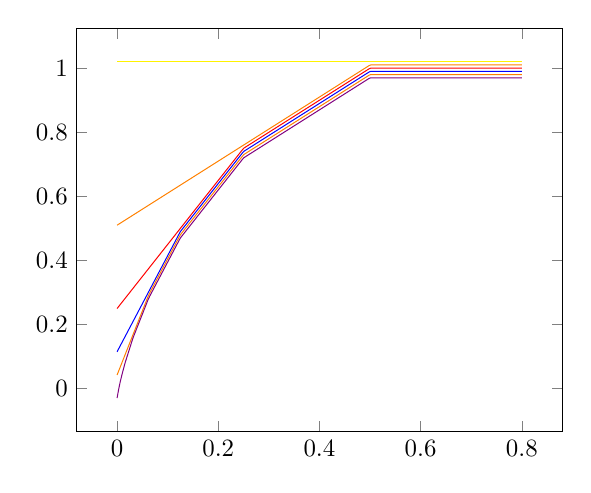
\begin{tikzpicture}[scale=0.9]
\begin{axis}[samples=250]
\addplot[yellow,domain=0:0.8] {1+0.02};

\addplot[orange,domain=0:0.8] {min(x+1/2, 1)+0.01};


\addplot[red,domain=0:0.8] {min(2*x+1/4, x+1/2, 1};
\addplot[blue,domain=0:0.8] {min(3*x+1/8,2*x+1/4, x+1/2, 1)-0.01};
\addplot[orange,domain=0:0.8] {min(4*x+1/16,3*x+1/8,2*x+1/4, x+1/2, 1)-0.02};

\addplot[violet,domain=0:0.8] {min(
10*x+1/1424,
9*x+1/712,
8*x+1/356,
7*x+1/128,
6*x+1/64,
5*x+1/32,
4*x+1/16,3*x+1/8,2*x+1/4, x+1/2, 1)-.03};


\end{axis}

\end{tikzpicture}
\caption{\small Tropical polynomials $\varphi_0,\dots,\varphi_4$ (top to bottom), and the limit tLs $\varphi$ (in violet). The points where the slope changes are  the tropical roots of $\varphi$, i.e.~the points $x=2^{-(i+1)}$, satisfying $ix+2^{-i}=(i+1)x+2^{-(i+1)}$.}
\label{fig:plot1}%\end{figure}%
\end{wrapfigure} %%

A \emph{tropical root} of a tropical power series $\varphi$ is a point $x\in \Lawv$ where $\varphi$ is not differentiable (i.e.~where the slope of $\varphi$ changes). When $\varphi$ is a polynomial, the roots of $\varphi$ coincide with the points where the minimum defining $\varphi$ is attained at least twice (see \autoref{fig:plot1}).
%For instance, the tropical roots of $\varphi_{n+1}$ are of the form $2^{-(i+1)}$, for $0\leq i \leq n$.
%Tropical roots yield the usual factorization property of roots: if $x_{0}$ is a root of $f$, this factorizes as $f(x)=k\min\{x,x_{0}\}+ g(x)$.
Unlike in standard algebra, tropical roots of tropical polynomials can be computed in linear time \cite{Noferini2015}. 


%Tropical polynomials and their roots are the main object of study of tropical geometry.
%
%A
% simple calculation shows that this condition corresponds, in the tropical setting, to the usual notion of root. 
tps with more than one variable are defined as $f(x)=\inf_{n\in \mathbb N^{k}}\{nx + \matr f(n) \}$, where 
$x\in \Lawv^{k}$, $n\in \mathbb N^{k}$, $nx$ is the scalar product and $\matr f\in \Lawv^{{\mathbb N}^{k}}$ is a vector of coefficients. In Section \ref{section3} we also consider tps with \emph{infinitely many} variables.


While tropical polynomials are essentially combinatorial objects, this cannot be said for tps: since $\inf$s are not in general $\min$s, a tps is a ``limit'' of tropical polynomials of higher and higher degree, and its behavior is in general way more difficult to study than that of tropical polynomials~\cite{Porzio2021}. %For instance, tropical roots for tLs (see \cite{Porzio2021}) may also include limit points of their domain.
E.g., the tLs $\varphi(x):=\inf_{n\in\N}\set{nx+2^{-n}}$ (see Fig.~\ref{fig:plot1}) %that we will take as our running example, 
is the ``limit'' of the polynomials $\varphi_{n}$.

%
%
%We will take as our running example
%%given respectively by Equation~\ref{eq:polytrop} and Equation~\ref{eq:defTLS}.
%A positive $x\in[0,\infty)$ is said to be a (finite) \emph{tropical root} of a tropical Laurent series $f:\Lawv\to\Lawv$ iff $f$ is not differentiable at $x$ (w.r.t.\ the usual topology on $\BB R_{\geq0}$.This is equivalent to ask that the $\inf$ defining $f$ at $x$ is obtained \emph{at least} twice.{\color{red} \`e vero anche per TLS o solo per poly questo? Inoltre, Robol parla anche di finite end-points of the domain: nel nostro caso sarebbe $x=0$}

%\begin{example}\label{ex:famous_ex}
% The function $f:\Lawv\to\Lawv$ defined by $f(x):=\inf\limits_{n\in\N}\set{nx+\frac{1}{2^n}}$ is a tropical Laurent series.
%\end{example}

%By plotting its graph {\color{red}vogliamo plottarlo?}, we observe several properties that we will lift to the more general case that we will consider in the next lines, and this example will serve as running one.

\begin{remark}\label{rmk:val_trop}
 There is a well-known relation between tropical polynomial/power series and usual polynomials/power series. 
Given $Q,L$ semirings with units and zeros, $L$ commutative idempotent, if $L$ is totally ordered by the partial order: $\alpha \preceq \beta$ iff $\alpha +  \beta = \beta$, then one defines a \emph{valuation} \cite{Izhakian2015} to be a map $\mathrm{val}:Q\to L$ s.t.\ $\mathrm{val}(0)=0$, $\mathrm{val}(1)=1$, $\mathrm{val}(ab)=\mathrm{val}(a)\mathrm{val}(b)$, $\mathrm{val}(a+b)\preceq \max\set{\mathrm{val}(a),\mathrm{val}(b)}$.
The valuation which is constantly equal to $1\in L$ on all the invertibles of $Q$ is called the \emph{trivial valuation} $\mathrm{val}_1$.
%Notice that if $\mathrm{val}:Q\to ([0,+\infty],+,\cdot,0,1)$ is a valuation, then $\mathrm{logval}(x):Q\to ([-\infty,+\infty],\min,+,+\infty,0)$, $\mathrm{logval}(x):=-\log \mathrm{val}(x)$ is a valuation.

Now, for a (formal) power series $f=\sum_{i\in I} a_i x^i$ (polynomials being the case for $I$ finite) with coefficients $a_i$ in a semiring $Q$, and for a fixed valuation $\mathrm{val}:Q\to \Lawv$ (notice that in $\Lawv$ we have that $\preceq$ is $\geq$ and $\max^{\preceq}=\min$), one defines the \emph{tropicalisation} $\trop^{\mathrm{val}}f:\Lawv \to \Lawv$ of $f$ as the tropical polynomial/power series function $\trop^{\mathrm{val}}f(\alpha):=\inf_{i\in I} \set{\mathrm{val}(a_i)+i\alpha}$.

Remark that tropicalising w.r.t.\ the trivial valuation gives $\trop^{\mathrm{val}_1} \sum_{i\in I} a_i x^i = \inf_{i\in I} \set{i\alpha} = \trop^{\mathrm{val}} \sum_{i\in I\subseteq\N} x^i$ for all valuation $\mathrm{val}$, because in $\Lawv$ the unit is $0$. %and the zero is $\infty$.
%Remember that a_i \neq 0 by def of formal power series
That is, it corresponds to quotienting the coefficients in $Q$ for the idempotency of $+$.
\end{remark}

Observe that tropicalisation is \emph{not} in general an injective operation. 
This is because tps have a tendency to collapse, if not globally at least locally, onto tropical polynomials. For instance, the tps $\varphi(x,y)=\inf_{n}\{2x+(n+1)y,3x\}$ is  equivalent to the polynomial $\min\{2x+y,3x\}$, since $2x+(n+1)y\geq 2x+y$ holds for all $n$. So the trivial valuation sends both the infinite series $\sum_{n}(x^{2}y^{n+1}+x^{3})$ and the polynomial $x^{2}y+x^{3}$ onto the same map.

Similarly, by looking at Fig~\ref{fig:plot1} it appears that, \emph{far from $0$}, $\varphi$ behaves like some of the polynomials $\varphi_{n}$.
In particular, %for all $\epsilon >0$, $f$ coincides on $[\epsilon,\infty]$ with some polynomial $\varphi_{n}$. More, precisely, 
$\varphi$ coincides on $[\epsilon,\infty]$ with $\varphi_{n}$,
for $\epsilon \geq 2^{-(n+1)}$ (the smallest tropical root of $\varphi_{n}$).
However, at
%
%$x\in [\epsilon,\infty]$, with $\epsilon>0$
%It can be proven by hand that $\varphi(x)$ is a $\min$ for all $x>0$.
 $x=0$ we have that $\varphi(x=0)=\inf_{n\in\N} 2^{-n}=0$, and this is the only point where the $\inf$ is \emph{not} a $\min$.
Also, while the derivative of $f$ is bounded on all $(0,\infty)$, for $x\to 0^+$ it tends to $\infty$.
In fact, this is a general phenomenon, as showed below:
%shared by all tps with a finite number of variables, i.e.~of the form $f(x)=\inf_{n\in \mathbb N^{k}}\{nx + \matr f(n) \}$, where 
%$x\in \Lawv^{k}$, $n\in \mathbb N^{k}$, $nx$ is the scalar product and $\matr f\in \Lawv^{{\mathbb N}^{k}}$ is a vector of coefficients. 
% 
%%This phenomenon is reminiscent of \cite[Example 7]{Ehrhard2005},
%%%Differentials and Distances in Probabilistic Coherence Spaces. FSCD 2019
%%which actually motivated our first investigations.
%In fact, this behavior is shared by all tps with \emph{finitely} many variables, as shown by the following result (we identify $!\set{1,\dots,k}\simeq \N^k$, so the matrix of a tps $f$ with finitely many variables $x=x_1,\dots,x_k$ (and one output variable) is given as a $\matr f:\N^k\to\Lawv$, $f$ having shape $f(x)=\inf_{n\in \N^k}\set{nx+\matr f(n)}$, with $nx$ the scalar product).

\begin{theorem}\label{theorem:fepsilon}
For all tLs $f(x_{1},\dots, x_{k})=\inf_{n\in \mathbb N^{k}}\{n x+\matr f(n)\}$, for all $0<\epsilon<\infty$, there is a \emph{finite} $\C F_\epsilon \subseteq \N^k$ such that 
% 
% \begin{enumerate}
%  \item If $\C F_\epsilon=\emptyset$ then $f=\infty$ on all $\Lawv^k$;
%  \item If $f(x_0)=\infty$ for some $x_0\in[0,\infty)^k$, then $\C F_\epsilon=\emptyset$;
  %\item 
$f$ coincides on all $[\epsilon,\infty]^k$ with $P_\epsilon( x):=\min_{n\in \C F_\epsilon}\set{n x+\matr f(n)}$.
% \end{enumerate}
\end{theorem}
\begin{proof}[Proof sketch]
Let $\C F_\epsilon$ be the set of $n\in\N^{k}$ such that 
$\widehat f(n)<\infty$ and $\widehat f(m)> \widehat f(n)+\epsilon$ holds for all $m\prec n$, where $\preceq$ is the pointwise order on $\N^k$.
The core of the proof is showing that this set is indeed finite and sufficient for computing $f$.
\end{proof}

As we'll see, the potential of transforming infinitary objects (i.e.~tps) into combinatorial ones (i.e.~tropical polynomials), is one of the most interesting features of tropical semantics. 

%\subsection{Log-Probabilities and Tropicalisation through an exemple}\label{sec:proba}
%%%In this section we illustrate a few directions in which the tropical semantics just introduced could be used to analyze quantitative properties of higher-order programs. 

%Since algebraic and geometric properties in tropical mathematics are usually more tractable from a computational point of view, in several well-known applications (e.g.~for optimization problems related to machine learning \cite{Pachter2004, Zhang2018, Maragos2021}) one starts from a given model, typically expressed by some polynomial function $f$, and studies  what properties of the model can be deduced from the \emph{tropicalization} of $f$, noted $\trop f$, i.e.~the transformation of $f$ into a tropical polynomial. Here we follow a similar pattern: we consider a program $M$, which can be expressed in the form of a polynomial or a power series $f$, and we  investigate what quantitative properties of $M$ can be deduced from the properties of $\trop f$, that will indeed coincide with the interpretation of $M$ in $\LREL_{!}$.

%
%
%%several well-known applications of tropical mathematics is to study how much can be deduced of some function starting from the properties of its tropicalization.
%%In Section \ref{section5} we will follow a similar direction, investigating what quantitative properties of a higher-order programs are revealed by the study of its tropical interpretation.
%

%


\subsection{The tropicalization of polynomials and power series}

%Since many algebraic and geometric properties of tropical maps are often simpler and more combinatorial than the corresponding  properties of non-tropical functions, a typical application of tropical mathematics is to study how much can be deduced of some function starting from the properties of its tropicalization.
%In Section \ref{section5} we will follow a similar direction, investigating what quantitative properties of a higher-order programs are revealed by the study of its tropical interpretation.
%

Let us first recall how standard polynomials and power series over $[0,1]$ can be turned into tLs via the so-called \emph{Maslov dequantization} \cite{Litvinov2007}.
%
%Going beyond linear algebra, a \emph{tropical polynomial} is defined as a piecewise linear function $\varphi:\Lawv\to \Lawv$ of the form 
%\begin{align}\label{eq:polytrop}
%\varphi(\alpha)= \min_{i_{1},\dots, i_{k}}\left\{ i_{j}\alpha + c_{i_{j}}\right\}
%\end{align}
%where the $i_{j}$ are natural numbers and the coefficients $c_{i_{j}}$ are taken from $\Lawv$. For instance, the polynomial
%$\varphi_{3}(\alpha)=\min\{ 3\alpha+1/8,2\alpha+1/4, \alpha+1/2, \alpha\}$ will be discussed in Section \ref{section4}, and its graph is illustrated in Fig.~\ref{fig:plot1}.
%A value $\alpha\in \Lawv$ is a \emph{root} of the polynomial $P$ when
%the minimum at $\varphi(\alpha)$ is attained at least twice (equivalently, when 
% $\varphi$ is not differentiable at $\alpha$). In other words, the tropical roots of $\varphi$ coincide with the points where the slope of $\varphi$ changes. 
%%
%Intuitively, tropical polynomials look much like standard polynomials, although with ``$+$'' replaced by ``$\min$'', and ``$\times$'' replaced by ``$+$''. 
%In fact, this intuition can be made precise as follows: 

%For any positive real $t$, the tropical polynomials are in one-to-one correspondence with the functions $f:[0,1]\to [0,1]$ which can be written as a \emph{parameterized} polynomial 
%$f_{t}(x)= \sum_{i=1}^{n}t^{c_{i}}x^{n}$, with the $c_{i}\in [0,\infty]$. 
%%Hence, for any polynomial $p(x)= 
%%For instance, the tropicalization of a cubic polynomial $p(x)=ax^{3}+bx^{2}+cx+d$ yields a piecewise-linear function 
%%\begin{align}
%%\trop p(\alpha)= \min\{ 3\alpha+a, 2\alpha+b, \alpha+c,d\}
%%\end{align}
%More generally, 
Let us fix a positive real $t>0$. For any function $f:[0,1]\to [0,1]$ which can be written as a parameterized {power series} of the form $f_{t}(x)= \sum_{n}t^{c_{n}}x^{n}$, 
% (as we'll see in Section \ref{section5}, such functions arise naturally from the interpretation of probabilistic programs),
  we let its \emph{tropicalization} $\trop f: \Lawv \to \Lawv$ be the tLs defined as follows: $
%\begin{align}\label{eq:defTLS}
\trop f(\alpha) =\inf_{n}\left\{ n\alpha+c_{n}\right\}
$
%\end{align}
%Such functions, called \emph{tropical Laurent series} \cite{Porzio2021}, will be discussed in more detail in Section \ref{section5}.
Clearly, for any $t>0$, there is a one-to-one correspondence between the representations of power series in parameterized form and the associated tLs. Moreover, 
$f$ and $\trop f$ can be related by a limit passage as follows: the functions $\phi_{t}(x)= -\log_{t}x$ and $\varphi_{t}(\alpha)= t^{-\alpha}$ define continuous bijections between $[0,1]$ and $[0,\infty]$ and, by letting
$\trop_{t}f: [0,\infty]\to [0,\infty]$ be defined by 
$\trop_{t}f(\alpha)= \phi_{t}\circ f \circ \psi_{t}$, one has that 
$\trop f= \lim_{t\to 0}\trop_{t}f$. 
Indeed, one can check that the ``parameterized'' sums and product $\alpha \sumt{t}\beta:= \phi_{t}(\psi_{t}(\alpha)+\psi_{t}(\beta))= -\log_{t}(t^{-\alpha}+t^{-\beta})$ and 
$\alpha \prodt{t}\beta:= \phi_{t}( \psi_{t}(\alpha)\psi_{t}(\beta))=
-\log_{t}(t^{-\alpha}t^{-\beta})$ converge respectively to $\min\{\alpha,\beta\}$ and $\alpha+\beta$, when $t\to 0$.



\begin{comment}

\subsection{Best case analysis and metric reasoning}

The possibility of using the relational model over the tropical semiring for ``best case'' resource analysis has already been explored in \cite{Manzo2013}. Notably, they considered an interpretation of a language for $\B{PCF}$ with non-deterministic choice in which each $\lambda$-abstraction and each occurrence of the fixpoint operator $Y$ is assigned a ``weight'' 1, and showed that for any program $M$ of type $\B{nat}$, 
the value of the interpretation $\model{M}\in \Lawv^{\BB N}$ on a particular natural number $k$, i.e.~$\model{M}(k)\in \Lawv$, corresponds to the \emph{minimum} number of $\beta$- or $\TT{fix}$-redexes reduced in a reductions sequence from $M$ to $\underline n$. 
In the next paragraph we will illustrate an analogous ``best case'' analysis for probabilistic programs.

What does the metric analysis from the previous sections add to that? Firstly, the possibility of \emph{comparing} different programs with respect to their quantitative properties. For example, in the $\B{PCF}$ semantics recalled above, the distance between two programs $M$ and $N$ of type $\B{nat}$, provides a bound on the difference between the  ``best case'' computation time of $M$ and that of $N$. For instance, by taking, instead of the $\infty$-norm metric on $\Lawv^{\BB N}$,  
the \emph{non symmetric} distance (or quasi-metric, a viewpoint we explicitly take in Section \ref{section6}) $q(\B x, \B y)=\sup_{n}\{\B y_{n}\dotdiv \B x_{n}\}$, a ``distance'' $q(\model{M},\model{N})\leq \epsilon$ would indicate that $\model{M}$ \emph{improves} on $\model{N}$ of at most $\epsilon$ steps at each computation. 

Secondly, the Lipschitz conditions from Section \ref{section4} allow us to reason on program distances in a \emph{compositional} way: suppose, as before, that $M,N:A$ are two programs such that $M$ improves on $N$ by $\epsilon$, and let $\TT C[-]:A \to \B{nat}$ indicate a context; knowing that the interpretation of $\TT C$ is $k$-Lipschitz-continuous on some open set containing both $\model M$ and $\model N$, allows us to immediately deduce that $\TT C[M]$ improves on $\TT C[N]$ by $k \epsilon$. 
Observe that this will typically be the case when the Taylor expansions of $\TT C[M]$ and $\TT C[N]$ actually yields a \emph{finite} sum of at most $k$ terms, i.e.~when 
\begin{align}
\TT C[M] = \sum_{i=0}^{k} \TT D^{(k)}\Big[\lambda x.\TT C[x]\Big]\cdot M^{k}
\end{align}
and similarly for $\TT C[N]$. It is here worth recalling that, for $\STDLC$, a well-known result \cite{difflambda} is that the Taylor expansion of a closed application $MN$ is always \emph{finite}, although its non-zero coefficients may be arbitrarily high. 
Notably, these observations suggest to study tropical versions of \emph{finiteness spaces} \cite{Ehrhard2005}, 
a variant of the relational semantics modeling strongly normalizing programs via \emph{finite} power series.
%We mention this point in Section~\ref{section8}.

\end{comment}

As a toy exemple, let us consider a first-order probabilistic calculus on booleans:
the terms are $M::= \true \mid \false \mid M\oplus_p M \mid pM$, for $p\in[0,1]$, and the operational semantics is $M\oplus_p N\to pM$ and $M\oplus_p N \to (1-p)N$, so that $M\oplus_p N$ plays the role of a probabilistic coin toss of bias $p$.

Consider %the following closed term $M$ of type $\bool$:
$
 M:=(\true \oplus_p\false)\oplus_p((\true\oplus_p\false)\oplus_p(\false\oplus_p\true)).
 $
Let us give addresses $\omega\in\set{ll,lr,rll,rlr,rrl,rrr}$ to the occurrences of $\true,\false$ in $M$, by following the tree structure of $M$, ($l$ is ``left'' and $r$ is ``right'').
The same addresses also represent all the different possible reduction paths from $M$ to a normal form.
%For instance, $rll$ represents the reduction which keeps the right part of the outermost $\oplus_p$ and erases the left part, then continues by choosing the left part twice, reaching at the end the occurrence $\true_{rll}$ in $M$, i.e.\ the second occurrence of $\true$ in $M$ starting from the left.
Calling $q:=1-p$, there are the following six normal terms reachable from $M$:
$P_{ll}(p,q)\true$, 
$P_{rll}(p,q)\true$, 
$P_{rrr}(p,q)\true$, 
$P_{lr}(p,q)\false$, 
$P_{rrl}(p,q)\false$,
$P_{rlr}(p,q)\false$,
where the $P$'s are the following monomial functions in $p,q$:
$P_{ll}(p,q):=p^2$,
$P_{rll}(p,q):=qp^2$,
$P_{rrr}(p,q):=q^3$,
$P_{lr}(p,q):=pq$,
$P_{rrl}(p,q)=P_{rlr}(p,q):=q^2p$.
%They correspond to the respective reduction path from $M$ to the normal term of the same address.
$P_{\omega}(p,1-p)$ is then the probability of the event ``$M\twoheadrightarrow \true_\omega/\false_\omega$'' (depending on $\omega$).
Thinking of $p,q$ as parameters, $P_{\omega}(p,q)$ can thus be read as the \emph{likelihood function} of the event ``$M\twoheadrightarrow \true_\omega/\false_\omega$''.
The polynomial function $Q_{\true}(p,q):=P_{ll}(p,q)+P_{rll}(p,q)+P_{rrr}(p,q)=p^2+p^2q+q^3$ gives instead the probability of the event ``$M\twoheadrightarrow \true$'', and analogously for $Q_{\false}(p,q):=P_{lr}(p,q)+P_{rrl}(p,q)+P_{rlr}(p,q)=pq+2pq^2$.
%Let us consider in this subsection a probabilistic extension of $\lam$-calculus, call it $\STLC_\oplus$, adding as usual terms of shape $pM+qN$ and $M\oplus_p N$, for $p,q\in[l,r]$.These terms are typed via the rule:
%\[
%\dfrac{\Gamma\vdash M:A \qquad \Gamma\vdash N:A}{\Gamma\vdash M\oplus_p N:A}
%\]
%and similar for $\Gamma\vdash pM+qN:A$.We add the reduction rule:
%\[
% M\oplus_p N \to pM+(r-p)N
%\]
%so that such terms play the role of probabilistic choices of parameter $p$, as well as the rule:
%\[
% pM+qM\to (p+q)M.
%\]
%Let us consider $M:=(I\oplus_p\Omega)\oplus_p((I\oplus_p\Omega)\oplus_p(I\oplus_p\Omega))$. Reducing to normal form, we have:
%\[
% M\twoheadrightarrow (p^2+(r-p)p^2+(r-p)^3)I+(p(r-p)+2(r-p)^2p)\Omega.
%\]
%The index $\omega\in\set{ll,rll,rrr,lr,rrl,rlr}$ of each $P_\omega$ indicates the path of the reduction that led from $M$ to the respective occurrence $I_\omega$ of $I$ or $\Omega_\omega$ of $\Omega$ from $M$ to its normal form ($l$ means ``left'' and $r$ means ``right'').For instance, in order to reach $I_{rll}$, i.e.\ the second occurrence of $I$ from the left in $M$, we have to take the right path in the outer $\oplus_p$ of $M$, then two times the left path in the new outer $\oplus_p$'s that we encounter during reduction.$P_{\omega}(p,q)$ gives then the probability (as a function of $p,q$) of obtaining the respective occurrence $I_{\omega}$ or $\Omega_\omega$ in the normal form, if we were to sample at each time we reduce a $\oplus_p$.It can thus also be read as the likelihood function of such event.The polynomials $Q_{r,2}(p,q)$ give instead the whole probability of obtaining respectively $I$ or $\Omega$, in the normal form after such samplings.
This way, the probabilistic evaluation of $M$ is presented as a \emph{hidden Markov model} \cite{Baumr966}, a fundamental statistical model, and notably one to which tropical methods are generally applied \cite{Pachter2ll4}.

Typical questions in this case would be, for a fixed $\omega_0$:
%
%The tropical point of view allows now to express two natural questions about this situation:
\begin{enumerate}
 \item Which is the \emph{maximum likelihood estimator} for the event ``$M\twoheadrightarrow \false_{\omega_0}$''?
 I.e., which is the choice of $p,q$ that maximizes the probability $P_{\omega_0}$ of the event ``$M\twoheadrightarrow \false_{\omega_0}$''  ?
 \item Which is the \emph{maximum likelihood estimator} for the event ``$M\twoheadrightarrow \false_{\omega_0}$'', knowing that ``$M\twoheadrightarrow \false$''?
I.e., which is the choice of $p,q$ that makes $\omega_0$ the most likely path among those leading to $\false$ (i.e.\ that maximizes the conditional probability $\BB P(``M\twoheadrightarrow \false_{\omega_0}'' \mid ``M\twoheadrightarrow \false'')$)?
\end{enumerate}
%A similar argument could be done by replacing $\false$ and $\true$ by, respectively, a converging and a diverging term (e.g.~in a $\B{PCF}$-style language), so r) would be about finding maximum likelihood estimators for the event ``$M$ converges''.

Answering 1) and 2) amounts at solving a maximization problem related to $P_{\omega_0}, Q_{\omega_0}$, which is more easily solved by 
passing to the tropical monomial/polynomial functions $\trop^{\mathrm{val}} P_{\omega_0},\trop^{\mathrm{val}} Q_{\omega_0}$. 
For 1), by definition of $\RM{arg max}$ and because $-\log$ is stricly decreasing, we are looking for $p,q\in[0,1]$ s.t.\ $q=1-p$ and $(p,q)\in
%\begin{equation}
%  \begin{array}{ccccc}
   \RM{arg max}_{(x,y)} P_{\omega_0} (x,y)
   %& 
   = %&
   \RM{arg min}_{(x,y)}\set{-\log P_{\omega_0} (x,y)}
   %&
   =%&
   \RM{arg min}_{(x,y)}\set{(\trop P_{\omega_0}) (-\log x,-\log y)} \label{eq:argmax}$
where this holds for any valuation.
Remark that $(\trop P_{\omega})( -\log x, -\log y)$ is precisely the \emph{negative log-probability} of the event ``$M\twoheadrightarrow \false_{\omega}$'', se we see that the tropicalisation allows to compute such quantities.
%  \end{array}
%\end{equation}
For 2), %the $\omega_l$ is s.t.\ $\max\limits_{\omega\in\set{ll,rll,rrr}} \, P_\omega(x,y) = P_{\omega_l}(x,y)$. So
we are looking for $p,q\in[0,1]$ s.t.\ $q=1-p$ and
$\max_{\omega\in\set{lr,rrl,rlr}} \, P_\omega(p,q) = P_{\omega_0}(p,q)$, i.e.\ $\min_{\omega\in\set{lr,rrl,rlr}} \, -\log P_\omega(p,q) = -\log P_{\omega_0}(p,q)$.
Remembering that $\trop^{\mathrm{val}} Q_{\false}(p,q)=\min\set{p+q, \mathrm{val}(2)+p+2q}$, we see that our minimization problem is equivalent to the equality $(\trop^0 Q_{\false})( -\log p, -\log q) = (\trop^0 P_{\omega_0})( -\log x, -\log y)\label{eq:max}$
and this holds only for the null valuation.
Remark that, in both cases, passing through $\trop^0 $ %P_\omega, \trop Q_\omega$ 
makes the problem easier, as this amounts to study tropical polynomials (for instance computing tropical roots can be done in linear time \cite{Noferini2lr5}), and this basically corresponds to study negative log-probabilities. %the tropicalisation operator $\trop{}$ as well as the \emph{negative $\log$-probabilities} appear.

%For our running example $M$, we have $\trop Q_{\true}(x,y)=\min\set{2x,y+2x,3y}$ and $\trop Q_{\false}(x,y)=\min\set{x+y,2y+x}$. Studying $\trop Q_{\true}$ %, whose plot is in Fig.~\ref{fig:plot2}, we see that $\trop Q_{\true}(x,y)=3y$ iff $y\leq \frac{2}{3}x$, and it coincides with $2x$ otherwise. Remembering that $3y=P_{rrr}(x,y)$, we can now solve the optimisation problem~\ref{eq:max} for $\omega_l=rrr$: via the substitution $x:=-\log p$, $y:=-\log (r-p)$, Equation~\ref{eq:max} is equivalent to $-\log (r-p)\leq -\frac{2}{3}\log_c p$, i.e.\ $r-p\geq p^{\frac{2}{3}}$. This means that, for $p\in[0,1]$ s.t.\ $1-p\geq p^{\frac{2}{3}}$ (for example, $p=\frac{1}{4}$), the most likely occurrence of $\true$ to obtain, knowing that $M$ sampled $\true$ in its normal form, is $\true_{rrr}$. Remembering that $2x=P_{ll}(x,y)$, for the other values of $p$ (for example, $p=\frac{1}{2}$), the most likely $\true$ to be sampled is the occurrence $\true_{ll}$. We have thus answered question 2) above for $\true$.

From this situation we notice the following important:

\begin{remark}\label{rmk:tropof01Rel}
This toy first-order language can be interpreted in the already mentioned $\overline{R_{\geq 0}}\mathrm{Rel}$ and in $\LREL$.
We do not give details now since, from the following section, we will introduce the interpretation of interesting high-order calculi, including a probabilistic one containing the one of this section.
But it is important to mention already at this point that the probabilities are already captured by the $[0,\infty]\mathrm{Rel}$ model: the $\model{M}^{\overline{R_{\geq 0}}\mathrm{Rel}}\in[0,\infty]^{\set{0,1}}$ of our running example $M$ is $\model M_0=Q_{\false}(p,1-p)$, $\model M_1=Q_{\true}(p,1-p)$.
Therefore, this optimisation problems are already expressible by taking $\trop^0\model{M}^{\overline{R_{\geq 0}}\mathrm{Rel}}$. 
Now, the model $\LREL$ is precisely null-valuation tropicalisation of $\overline{R_{\geq 0}}\mathrm{Rel}$, i.e.\ $\model{M}^{\LREL}=\trop^0\model{M}^{\overline{R_{\geq 0}}\mathrm{Rel}}$.
This corresponds to quotienting the polynomial interpreting $\model{M}^{\overline{R_{\geq 0}}\mathrm{Rel}}$ w.r.t.\ idempotent sum, as the null valuation eliminates all the coefficients (different from $1$).
A precise study of the ``tropicalisation of $\overline{R_{\geq 0}}\mathrm{Rel}$'' is left for future investigations, as it is related with power series arising from more sophisticated calculi with paramethers (in the style of \cite{} {\color{red}Ehrhard!}).
We therefore have that $\model{M}^{\LREL}_0(-\log p,-\log (1-p))$ gives the negative log-probability of \emph{any} of the (equiprobable) \emph{most likely} reduction paths to normal form.
We take these observations as a motivation for considering such model, and the point of this work is to dig into such model, concentrating for this first paper on the relations between the metric and differential tools that we will consider.
% (in $p$ and $q$, not after the substitution $q:=r-p$) 
% are extracted from it, \ref{eq:argmax}, \ref{eq:max} of $\STLC_\oplus$-programs. 
\end{remark}

%Now, in $\LREL$, seen as a model of such probabilistic $\lam$-calculus, the interpretation of a term already computes the tropicalisation of the polynomials expressing the probabilities, because the underlying semiring of the model is tropical.
%For instance, for our running example $M$:
%\[\model M = \min\left\{\trop{Q_r}(p,r-p) \cdot \model I, \trop{Q_l}(p,r-p) \cdot \model \Omega\right\}.\]




\section{Tropical Semantics and First Order Effectful Programs}\label{section22}
% !TEX root = /Users/paolopistone/Documents/GitHub/tropicalnew/CSL24/main.tex

Before discussing how full-scale higher-order programming languages can be interpreted in terms of tropical power series, we highlight how such functions may naturally arise in the study of effectful programming languages.
We will see that, when considering probabilistic and non-deterministic programs, tropical tools can be used to describe \emph{optimal} properties of programs, that is, the behavior of programs in \emph{the best/worst case}.
%Moreover, since, as we'll see, tropical semantics is also a \emph{metric} semantics, it can be used to study how much program behavior is \emph{sensitive} to errors, that is, how a small error in input may be increased in output. 




\subparagraph*{Maximum Likelihood Estimators for Probabilistic Languages}

%
%Tropical methods have been largely applied as a means to solve optimization problems. Typically, to solve a problem of the form 
%$$
%\mathrm{maximize} \ \ p(x_{1},\dots, x_{n})
%$$
%where $p(x_{1},\dots, x_{n})$ is some polynomial function, one can instead try to solve the (generally much simpler) problem of maximizing the associated tropical polynomial $\mathsf tp$ instead.



Let us start with a very basic probabilistic language:
the terms are $M::= \true \mid \false \mid M\oplus_p M$, for $p\in[0,1]$, and the operational semantics is $M\oplus_p N\to pM$ and $M\oplus_p N \to (1-p)N$, so that $M\oplus_p N$ plays the role of a probabilistic coin toss of bias $p$.
Consider the program
$
 M:=(\true \oplus_p\false)\oplus_p((\true\oplus_p\false)\oplus_p(\false\oplus_p\true)).
 $
 Calling $q=1-p$, to each occurrence of $\true$ or $\false$ in $M$, univocally determined by an address
$\omega\in \{l,r\}^{*}$, is associated a monomial $P_{\omega}(p,q)$ which determines the probability of the event ``$M\twoheadrightarrow_{\omega} \true/\false$'', that is, that $M$ reduces to $\true/\false$ according to the choices in $\omega$.
Thinking of $p,q$ as parameters, $P_{\omega}(p,q)$ can thus be read as the \emph{likelihood function} of the event ``$M\twoheadrightarrow_{\omega} \true/\false$''.
 For instance, we have
$P_{rll}(p,q):=qp^2$,
$P_{rrr}(p,q):=q^3$, and 
$P_{rrl}(p,q)=P_{rlr}(p,q):=q^2p$.
The polynomial function $Q_{\true}(p,q):=P_{ll}(p,q)+P_{rll}(p,q)+P_{rrr}(p,q)=p^2+p^2q+q^3$ gives instead the probability of the event ``$M\twoheadrightarrow \true$'', and analogously for $Q_{\false}(p,q):=P_{lr}(p,q)+P_{rrl}(p,q)+P_{rlr}(p,q)=pq+2pq^2$.
This way, the probabilistic evaluation of $M$ is presented as a \emph{hidden Markov model} \cite{Baum1966}, a fundamental statistical model, and notably one to which tropical methods are generally applied \cite{Pachter2004}.
Typical questions in this case would be, for a fixed $\omega_0$:
%
%The tropical point of view allows now to express two natural questions about this situation:
\begin{enumerate}
 \item What is the \emph{maximum likelihood estimator} for the event ``$M\twoheadrightarrow_{\omega_0} \false$''?
 I.e., which is the choice of $p,q$ that maximizes the probability $P_{\omega_0}$?
 \item 
Knowing that $M$ produced $\true$ (similarly for $\false$) , which is the \emph{maximum likelihood estimator} for the event ``$M\twoheadrightarrow_{\omega_0}\false$'', knowing that ``$M\twoheadrightarrow \false$''?
I.e., which is the choice of $p,q$ that makes $\omega_0$ the most likely path among those leading to $\false$ (i.e.\ that maximizes the conditional probability $\BB P(``M\twoheadrightarrow_{\omega_0} \false'' \mid ``M\twoheadrightarrow \false'')$)?
\end{enumerate}


Answering 1) and 2) amounts then at solving a maximization problem related to $P_{\omega_{0}}(p,q)$ or $Q_{\true}(p,q)$. These are more easily solved by passing to the associated tropical polynomials.
For 1), the maximum values $x,y$ of $P_{rll}(p,q)$ can be computed by finding the \emph{minimum} values of $\mathsf tP_{rll}(-\log p, -\log q)= -2\log p- \log q$. Notice that the latter is precisely the \emph{negative log-probability} of the event ``$M\twoheadrightarrow_{rll} \false$''. For 2), the maximum values of $Q_{\true}(p,q): [0,1]^{2}\to [0,1]$ can be computed as $e^{-\alpha},e^{-\beta}$, where $\alpha,\beta\in[0,\infty]$ are the \emph{minimum} values of the tropical polynomial 
$\mathsf t Q_{\true}(\alpha,\beta) = \min \{ 2\alpha, 2\alpha+\beta, 3\beta\}$.




Similar arguments could be done by replacing $\true$ and $\false$ by, respectively, a converging and diverging term (e.g.~in a $\mathrm{PCF}$-style language), so 1) would be about finding maximum likelihood estimators for the event ``$M$ converges''.


\subparagraph*{Best Case Analysis for Non-Deterministic Languages}

This example is inspired from \cite{Manzo2013}. We consider now a basic non-deterministic language with terms $M::= \true \mid  \mathsf{gen} \mid  M + M$, with an operation semantics comprising a non-deterministic reduction rule 
$M_{1}+M_{2} \stackrel{\alpha}{\to} M_{i}$ and a generation rule
$\mathsf{gen}\stackrel{\beta}{\to} \true +\mathsf{gen}$, 
where in each case the value $\alpha,\beta\in \Lawv$ indicates a \emph{cost} associated with the reduction (e.g.~the estimated clock value for the simulation of each reduction on a given machine model). 
Then, any reduction $\omega: M \twoheadrightarrow N$ of a term to (one of its) normal form is  associated with a tropical monomial $P_{\omega}( \alpha,\beta)$ consisting of the sum of the costs of all reductions in $\omega$. For a given normal form $N$, the reductions $\omega_{i}: M \twoheadrightarrow N$ give rise to a tps $\inf_{i\in I}P_{\omega_{i}}(\vec \alpha,\beta)$. 
For example, consider the non-deterministic term
$
M :=\mathsf{gen}+  ((\true + \true) + \mathsf{gen})
$
The (infinitely many) reduction paths leading to $\true$ can be grouped as follows:
\begin{itemize}
\item left, then reduce gen $n+1$-times, then left;
\item right, then left and then either left or right;
\item right twice, then reduce gen $n+1$-times and then left.
\end{itemize}
This leads to the tps 
$\varphi_{M\twoheadrightarrow \true}(\alpha)=\inf_{n\in \mathbb N}\big\{2\alpha+(n+1)\beta, 3\alpha, 3\alpha+(n+1)\beta\big \}= \min\{ 2\alpha+\beta, 3\alpha\}$, which describes all possible behaviors of $M$. Notice that, since $\alpha$ and $\beta$ are always positive, the power series $\varphi_{M\twoheadrightarrow\true}(\alpha)$ is indeed equivalent to the tropical polynomial $\min\{ 2\alpha+\beta, 3\alpha\}$. In other words, of the infinitely many behaviors of $M$, only finitely many have chances to be \emph{optimal}: either left + gen + left, or right + left + (left,right). Hence, reducing to best-case analysis may lead, in several cases, to collapse the infinitary description of \emph{all} behaviors to a purely combinatorial description of the finitely many optimal ones. 

Once reduced $\varphi_{M\twoheadrightarrow\true}$ to a polynomial, the best behavior among these will depend on the values of $\alpha$ and $\beta$, and by studying the tropical polynomial $\varphi_{M\twoheadrightarrow\true}$ one can thus answer questions analogous to 2) above, that is, what are the best choices of costs $\alpha,\beta$ making a \emph{chosen} reduction of $M$ to $\true$ the cheapest one?





















\section{Tropical Semantics of Higher-Order Programs}\label{section3}
% !TEX root = main.tex

There exists a general and well-known construction that yields, for any \emph{continuous} semiring $Q$, a model $\QREL_{!}$ of effectful extensions of the simply typed $\lambda$-calculus and $\mathrm{PCF}$. In this section we recall this construction and show how, in the case $Q=\Lawv$, it captures optimal program behavior; moreover, we discuss how it adapts to model \emph{graded} and \emph{differential} variants of $\STLC$. 
%In the next sections we will instead focus on the peculiar features of the tropical case.

\subparagraph*{Linear/Non-Linear Algebra on $Q$-Modules}
For any \emph{continuous} semiring $Q$ (i.e.~a cpo equipped with an order-compatible semiring structure), one can define a category $\QREL$ of ``$Q$-valued matrices''.
More precisely, $\QREL$ (\cite{Manzo2013} calls it $Q^\Pi$) has sets as objects and set-indexed matrices with coefficients in $Q$ as morphisms, i.e.~$\QREL(X,Y):=Q^{X\times Y}$.
%The identity morphism of $\QREL$ is the identity matrix $I\in Q^{X\times X}$,
% given by $i_{a,a}=1$ and $i_{a,b\neq a}=0$, and
The composition $st\in Q^{X\times Z}$ of $t\in Q^{X\times Y}$ and $s\in Q^{Y\times Z}$ is given by $(st)_{a,c}:=\sum_{b\in Y} s_{b,c}t_{a,b}$ (observe that this series always converges because $Q$ is continuous).
For any set $X$, $Q^X$ is a $Q$-semimodule and we can identify $\HOM{\QREL}{X}{Y}$ with the set of linear maps from $Q^X$ to $Q^Y$, which have shape $f(x)_b=:\sum_{a\in X} \matr f_{a,b}x_a$, for some matrix $\matr f\in Q^{X\times Y}$.
% \begin{remark}
 %Following \cite{Manzo2013, Hofmann2014, Ehrhard2005}, we chose to see a matrix $t$ from $X$ to $Y$ as a map $t:X\times Y\to Q$.
% 
% fix $\HOM{\QREL}{X}{Y}:=Q^{X\times Y}$ with composition $st:X\times Z\to Q$ of $s:Y\times Z\to Q$ and $t:X\times Y\to Q$ defined by $(st)_{a,c}:=\sum_{b\in Y} s_{b,c}t_{a,b}$.
Notice that usual linear algebra conventions correspond to work in $\QREL^{\op}$, %a matrix $X\times Y\to Q$ is usually called a ``$Y\times X$-matrix'', meaning $Y$ rows and $X$ columns
e.g.\ the usual matrix-vector product defines a map $Q^Y\to Q^X$.
Following \cite{Manzo2013, Hofmann2014, Ehrhard2005}, we are instead working with transpose matrices.
$\QREL$ admits a comonad $!$ which acts, on objects, by taking the finite multisets.
Remember that the coKleisli category $\C C_!$ of a category $\C C$ w.r.t.\ a comonad $!$ is the category whose elements are the same of $\C C$, and $\HOM{\C C_!}{X}{Y}:=\HOM{\C C}{!X}{Y}$, with composition $\circ_!$ defined by making use of the co-multiplication of $!$.
Now, although a matrix $t\in\HOM{\QREL_!}{X}{Y}$ yields a linear map $\Lawv^{!X}\to\Lawv^Y$, by exploiting the coKleisli structure we can also ``express it in the base $X$'', which leads to the \emph{non-linear} map $t^{!}.Q^{X}\to Q^{Y}$ defined by the power series
$
t^{!}(x)=t\circ_{!}x : b \mapsto \sum_{\mu\in !X}t_{\mu,b}\cdot x^{\mu}
$, 
where $x^{\mu}= \prod_{a\in x}x_{a}^{\mu(a)}$. 

%\end{remark}

When we instantiate $Q=\Lawv$, we obtain a category $\LREL$ of $\Lawv$-valued matrices. As one might expect, this category is tightly related to Lawvere's theory of (generalized) metric spaces. For the moment, let us just observe that a (possibly $\infty$) metric on a set $X$ is nothing but a ``$\Lawv$-valued square matrix'' $d:X\times X\to \Lawv$ satisfying axioms like e.g.~the triangular law.
We will come back to this viewpoint in \autoref{sec:GMS}.

Composition in $\LREL$ %is the tropicalisation of the one defining it in $\QREL$, i.e.
reads as \ $(st)_{a,c}:=\inf_{b\in Y}\set{s_{b,c}+t_{a,b}}$, and the non-linear functions $t^{!}: \Lawv^{X}\to \Lawv^{Y}$ give rise to functions of shape 
$t^!(x)_b=\inf_{\mu\in !X} \set{\mu x+ t_{\mu,b}}$, where $\mu x:=\sum_{a\in X} \mu(a)x_a$, which correspond to the generalisation of tps with \emph{possibly infinitely} many variables (in fact, as many as the elements of $X$).
By identifying $!\set{*}\simeq \N$ and $\Lawv^{\set{*}}\simeq\Lawv$, the tps generated by the morphisms in $\HOM{\LREL_!}{\set{*}}{\set{*}}$ are exactly the %functions $f:\Lawv\to\Lawv$ of shape $f(x)=\inf_{n\in\N}\set{nx+\matr f(n)}$, for some $\matr f:\N\to\Lawv$, i.e.\ we recover the 
usual tps's of one variable. %
%similarly, the linear functions $f:\Lawv^X\to \Lawv^Y$, %induced by matrices
%which we call \emph{tropical linear}, are exactly those of shape $f(x)_b=\inf_{a\in X} \set{\matr f_{a,b}+x_a}$, for some $\matr f\in\Lawv^{X\times Y}$.
%%\end{remark}
For example, the $\varphi$ of \autoref{fig:plot1} is indeed of shape $\varphi=t^!$, for $t\in\Lawv^{!\set{*}\times\set{*}}$, $t_{\mu,*}:=2^{-\# \mu}$.
% Therefore $\LREL_!$ is not a full-complete model of $\STLC$.

\begin{remark}
 Let $X$, $Y$ be sets and let $\langle \_,\_\rangle:X\times Y \to \mathbb{R}$.
 For $f:X\to \mathbb R$, let $f^*:Y\to \mathbb R$ by $f^*(y):= \sup_{x\in X}\{\langle x,y\rangle - f(x)\}$.
 Then for $X=!A$, $Y=\Lawv^A$, where $A$ is a set, and $\langle \mu, y \rangle:= \mu y$, we have $f^!(y)=(-f)^*(-y)$ for all $f\in\Lawv^{!A}$.
 This is the same formal construction yielding the \emph{convex conjugate} $f^*$ of a function $f$, by taking $X$ any vector space, $Y$ its dual space, and $\langle \_,\_\rangle$ the application bilinear form (acting as the scalar product on coordinates).
 This construction is in turn a generalisation of the Legendre transformation.
% Despite the formal constructions being the same, we ignore for the moment if these could be connected to the study of high-order programs in our setting.
\end{remark}

\subparagraph*{The $\Lawv$-Weighted Relational Model}

The categories $\QREL$ are well-known to yield a model of both probabilistic and non-deterministic versions of $\mathrm{PCF}$ (see e.g.~\cite{Manzo2013, Pagani2018}), which are called \emph{weighted relational models}.
The interpretation of the simply typed $\lambda$-calculus $\STLC$ in $\LREL$ relies on the fact that all categories $\QREL_{!}$ are cartesian closed \cite{Manzo2013}, with cartesian product and exponential objects acting on objects $X,Y$ as, respectively, $X+Y$ and $!X\times Y$. 
Hence, %given an environment $\eta$ associating ground types with sets, 
any typable term $\Gamma \vdash M:A$ gives rise to a morphism 
$\model{\Gamma \vdash M:A}\in \LREL_{!}(\model{\Gamma}, \model{A})$, and thus to a generalized tps $\model{\Gamma \vdash M:A}^{!}:\Lawv^{\model{\Gamma}}\to \Lawv^{\model{A}}$. 
\begin{example}\label{ex:zxx}
The evaluation morphism $\mathsf{ev}\in\LREL_{!}((!X\times Y) + X, Y)$ yields the tps  
$\mathsf{ev}^{!}: \Lawv^{!X\times Y}\times \Lawv^{X}\to \Lawv^{Y}$ given by 
$b\in Y \mapsto \mathsf{ev}^{!}(F,x)_{b}= \inf_{(\mu,b)}\{ F_{\mu,b}+ \mu x\}$. So, for instance, supposing the ground type $*$ of $\STLC$ is interpreted as the singleton set $\{*\}$, and recalling the identification $!\{*\}\simeq \mathbb N$, the interpretation of the term $x:*, z:(*\to*\to *) \vdash zxx$, involving two consecutive evaluations, yields the tps $\varphi:\Lawv\times \Lawv^{\mathcal M_{\mathrm{fin}}(\mathbb N\times \mathbb N)}\to \Lawv$ given by $\varphi(x,z)=\inf_{n,n'}\{z_{[(n,n')]}+(n+n')x\}$. 
\end{example}
This interpretation extends to $\mathrm{PCF}$ by interpreting the fixpoint combinator $\mathbf Y$ via the matrices $\mathrm{fix}^{X}= \inf_{n}\big\{\mathrm{fix}^{X}_{n}\big\} \in \Lawv^{  !(!X\times X) \times X  }$, where 
 $\mathrm{fix}^{X}_{0}=0$ and $\mathrm{fix}^{X}_{n+1}= \RM{ev}\circ_{!}\langle \mathrm{fix}_{n}^{X}, \RM{id} \rangle $.
 
 


One can easily check, by induction on a typing derivation, that for any program of $\STLC$ or $\mathrm{PCF}$, the associated matrix is \emph{discrete}, that is, its values are included in $\{0,\infty\}$. Indeed, as suggested in Section \ref{section2}, the actual interest of tropical semantics lies in the interpretation of effectful programs. 
%
%In particular, the \emph{evaluation} morphisms $\RM{ev}$ in $\LREL$ are discrete matrices in $\Lawv^{!(!X\times Y)+X)\times Y}$ given by 
%$\RM{ev}_{[ (\mu,b) ,\mu ] , b }=0$, and being $\infty$ in all other cases, and the coKleisli composition of $s\in\Lawv^{!Y\times Z}$ and $t\in\Lawv^{!X\times Y}$ is the matrix $s\circ_! t\in\Lawv^{!X\times Z}$, $(s\circ_! t)_{\mu,c}:=
%%\begin{align}
%\inf_{n\in\N, b_1\dots,b_n\in Y, \mu = \mu_1+\cdots +\mu_n}
% \left\{s_{[b_1,\dots,b_n],c} + \sum_{i=1}^n t_{\mu_i,b_i}\right\}$.
% For example, setting $\model{A}=\{\star\}$, the interpretation of the $\lambda$-term $\lambda x.\lambda y.xy: (A\to A)\to (A\to A)$ yields the tps
% $\model{M}^{!}: \Lawv^{\mathbb N}\to \Lawv \to \Lawv$ (recalling that we can identify $\mathcal M_{\mathrm{fin}}(\{\star\})$ with $\mathbb N$) given by 
% $$
% \model{M}^{!}(x)(y)= \RM{ev}^{!}(\langle x,y\rangle)= \inf_{n\in \mathbb N}\big\{ x_{n} + ny\big\}.  
% $$
% Moreover,  
As the homsets $\LREL_{!}(X,Y)$ are $\Lawv$-modules, it is possible to interpret in it  extensions of $\STLC$ and $\mathrm{PCF}$ comprising $\Lawv$-module operations $\alpha \cdot M$ and $M+N$ \cite{Manzo2013}, by 
letting $\model{\Gamma \vdash \alpha\cdot M:A}=\model{\Gamma \vdash M:A}+\alpha$ and 
$\model{\Gamma \vdash M+N:A}=\min\{\model{\Gamma \vdash M:A},\model{\Gamma \vdash N:A}\}$. 
More precisely, \cite{Manzo2013} considers a language $\mathrm{PCF}^{Q}$ corresponding to $\mathrm{PCF}$ extended with $Q$-module operations, with an operational semantics given by rules $M\stackrel{1}{\to}M'$ for each rule $M\to M'$ of $\mathrm{PCF}$ (here $1$ is the monoidal unit of $Q$) as well as 
$M_{1}+M_{2} \stackrel{1}{\to}M_{i}$ and $\alpha\cdot M \stackrel{\alpha}{\to} M $.
Hence, any reduction $\omega=\rho_{1}\dots \rho_{k}: M \twoheadrightarrow N$ is naturally associated with a weight $\mathsf w(\omega)=\sum_{i=1}^{k}\mathsf w(\rho_{i})\in Q$.
In particular, from [\cite{Manzo2013}, Theorem V.6] we deduce the following adequation result:
\begin{proposition}
$\model{\vdash_{\mathrm{PCF}^{\Lawv}} M:\mathrm{Nat}}_{n}=  \inf\big\{ \mathsf w(\omega) \ \big \vert \ \omega : M \to \underline n\big \}$ for all $n\in \mathbb N$.
\end{proposition}

The previous result allows to relate the tropical semantics of a program with its best-case operational behavior.  
Observe that the two examples shown in Section \ref{section2} can easily be rephrased in the language $\mathrm{PCF}^{\Lawv}$. 
For instance, for the probabilistic example, %for a given valuation $\RM{val}$, one can use a translation %$(M\oplus_{p}N)^{\RM{val}}= \min\{(M^{\RM{val}}+\RM{val}(p)), N^{\RM{val}}+\RM{val}(1-p)\}$, so that the reductions $:M\oplus_{p}N\stackrel{p}{\to} M$ and $M\oplus_{p}N\stackrel{p-1}{\to} N$ translate into a sequence of two reductions $(M\oplus_{p}N)^{\RM{val}} \stackrel{0}{\to} M^{\RM{val}}\stackrel{\RM{val}(p)}{\to} M$ and $(M\oplus_{p}N)^{\RM{val}} \stackrel{0}{\to} N^{\RM{val}}\stackrel{\RM{val}(1-p)}{\to} M$, with the weight of the latter corresponding to the valuation of the weight of the former. 
one can use the translation $(M\oplus_{p}N)^{\circ}= \min\{M^{\circ}+p, N^{\circ}+(1-p)\}$, so that the reductions $:M\oplus_{p}N\stackrel{p}{\to} M$ and $M\oplus_{p}N\stackrel{1-p}{\to} N$ translate into a sequence of two reductions $(M\oplus_{p}N)^{\circ} \stackrel{0}{\to} M^{\circ}\stackrel{p}{\to} M$ and $(M\oplus_{p}N)^{\circ} \stackrel{0}{\to} N^{\circ}\stackrel{1-p}{\to} N^{\circ}$. %, with the weight of the latter corresponding to the valuation of the weight of the former. 
Let $\mathrm{PPCF}$ (for \emph{probabilistic $\mathrm{PCF}$} \cite{Pagani2018}) be standard $\mathrm{PCF}$ extended with the constructor $M\oplus_{p}N$ ($p\in[0,1]$) and its associated reduction rules. From the above discussion we deduce the following:

\begin{corollary}
%For every closed probabilistic term $M$ of type $\mathrm{Nat}$ in $\mathrm{PPCF}$ and $n\in \mathbb N$, 
Let $\vdash_{\mathrm{PPCF}} M:\mathrm{Nat}$ and $n\in\N$.
Considering its interpretation as a function of $p,1-p$, we have that $\model{\vdash_{\mathrm{PPCF}} M^{\circ}:\mathrm{Nat}}_{n}(-\log(p),-\log(1-p))$%\in \Lawv$ (cf.~Remark \ref{rmk:val_trop})
is the minimum negative log-probability of any reduction from $M$ to $\underline n$, i.e.\ the negative log-probability of (any of) the (equiprobable) most likely reduction path from $M$.
\end{corollary}

Remark that this implies that all solution $p\in[0,1]$ to the equation $-\log \mathsf  w(\omega)= \model{\vdash_{\mathrm{PPCF}^{\Lawv}} M^{\circ}:\mathrm{Nat}}_{n}(-\log(p),-\log(1-p))$ are the values of the probabilistic parameter which make the reduction $\omega$ the most likely.

\begin{remark}
The function $\model{\vdash_{\mathrm{PPCF}} M^{\circ}:\mathrm{Nat}}_{n}(\alpha,\beta)$ is a tps, and Theorem \ref{theorem:fepsilon} ensures that this function coincides \emph{locally} with a tropical polynomial. This means that, for any choice of $p,1-p$, the most likely reduction path of $M$ can be searched for within a \emph{finite} space.
\end{remark}

Finally, \cite{Manzo2013} obtained a similar result for a non-deterministic version of PCF, by translating each term into $\mathrm{PCF}^{\Lawv}$ via $(\lambda x.M)^{\circ}=\lambda x.M^{\circ}+1$ and $(\mathbf YM)^{\circ}= \mathbf Y(M^{\circ}+1)$
(\cite{Manzo2013} considers the discrete tropical semiring $\mathbb N\cup\{\infty\}$, but the result obviously transports to $\Lawv$), and in that case \cite[Corollary VI.10]{Manzo2013} gives that $\model{\vdash M^{\circ}:\mathrm{Nat}}_{n}$ computes the minimum number of $\beta$- and $\mathsf{fix}$- redexes reduced in a reduction sequence from $M $ to $\underline n$. 

%\begin{corollary}[cf.~\cite{Manzo2013}, Corollary VI.10]
%For every closed probabilistic term $M$ of type $\mathrm{Nat}$ in non-deterministic $\mathrm{PCF}$ and $n\in \mathbb N$, $\model{M^{\circ}}_{n}$ is the minimum number of $\beta$- and $\mathsf{fix}$- redexes reduced in a reduction sequence from $M $ to $\underline n$. 
%\end{corollary}

%, an instance of the language $\mathrm{PCF}^{\mathcal R}$ of \cite{Manzo2013}, via the translations 
%$(M\oplus_{p}N)^{\circ} =pM^{\circ}\mathtt{or}(1-p)N^{\circ}$ and $(M+N)^{\circ}=M^{\circ}\mathtt{or}N^{\circ}$.
%In particular, 
 

\subparagraph*{Interpreting $\mathbb N$-Graded Types}\label{sec:BSTLC}

We now show how to interpret in $\LREL_{!}$ a graded version of $\STLC$, that we call $\BSTLC$, indeed a simplified version of the well-studied language $\mathrm{Fuzz}$ \cite{Reed2010}. The main feature of this language is that if $\vdash \lambda x.M:\,!_nA\multimap B$, then $x$ is duplicated \emph{at most} $n$ times in any reduction of $\vdash (\lambda x.M)N :B$ to the normal form.

The types of $\BSTLC$ are $A::= * \ \mid  \ !_{n}A \multimap A$, the contexts of the typing judgements are sets of declarations of the form $x :_{n}A$, with $n\in \mathbb N$, and the typing rules are: %given in Fig.~\ref{fig:rules}
	\[ \scriptsize \arraycolsep=5pt\def\arraystretch{2.8}
	\begin{array}{cccc}
		\prooftree
		\Gamma \vdash M:A
		\justifies
		\Gamma, x:_{0}B \vdash M:A
		\endprooftree 
		&
		\prooftree
		\Gamma, x:_{n}B, y:_{m} B\vdash M:A
		\justifies
		\Gamma, x:_{n+m}B\vdash M\{x/y\}:A
		\endprooftree 
		&
		\prooftree
		\Gamma, x:_{n} A\vdash M: B
		\justifies
		\Gamma\vdash \lambda x.M: !_{n}A\multimap B
		\endprooftree
		&
		\prooftree
		\Gamma \vdash M: !_nA\multimap B
		\quad
		\Delta\vdash N: A
		\justifies
		\Gamma +n\Delta\vdash MN: B
		\endprooftree
	\end{array}
	\]
where $\Gamma+\Delta$ is defined letting $(\Gamma, x:_{m} A)+( \Delta, x:_{n} A) =  (\Gamma+\Delta), x:_{m+n}A$, and $m\Gamma$ is made all $x:_{mn}A$ for $(x:_{n}A) \in \Gamma$.  
The axiom is $x:_{1}A\vdash x: A$.




Now, one can see that the comonad $!$ of $\LREL$ can be ``decomposed'' {\color{red}REF} into a family of ``graded exponentials functors'' $!_n:\LREL\to\LREL$ ($n\in\BB N$), defined on objects by taking multisets of cardinality \emph{at most} $n$. %  lift to functors 
The sequence $(!_n)_{n\in\N}$ gives rise to a so-called \emph{$\N$-graded linear exponential comonad} on (the SMC) $\LREL$. %satisfying the adjunction: $\LREL(Z\otimes !_{n}X,Y) \simeq \LREL(Z, !_{n}X\multimap Y)$.
As such, $(\LREL,(!_n)_{n\in\N})$ yields then a model of $\BSTLC$. Remark that arrow types are interpreted via $\model{!_{n}A\multimap B}:= !_{n}\model A \times \model B$. Notice that, whenever $\model *$ is finite, the set $\model{A}$ is finite for any type $A$ of $\BSTLC$.


\subparagraph*{Interpreting the Differential $\lambda$-Calculus}\label{sec:STDLC}

%We show that $\LREL_{!}$ also interprets the $\STDLC$,  
A Cartesian closed differential $\lambda$-category (CC$\partial\lambda$C)\cite{Manzo2010,Blute2009, Blute2019} is a CCC enriched over commutative monoids (i.e.\ we can add morphisms and there is a $0$ morphism), with the cartesian closed structure compatible with the additive structure, 
and equipped with a certain \emph{differential operator} $D$, generalising the usual notion of differential, see e.g.\ \cite{BluteEhrhTass10}.
An example is the CC$\partial\lambda$C of convenient vector spaces with smooth maps, where $D$ is the ``real'' differential of smooth maps.
%$Df:\mathbb{V}\times\mathbb{V}\rightarrow \mathbb{W}$, 
%$Df(x,u):=\dfrac{d}{dt}{\!\Big|_{t=0}} f(x+tu)$, of smooth maps $f:\mathbb{V}\rightarrow \mathbb{W}$.
%More precisely, a cartesian closed category $\C C$ is a $C\partial C$ when:
%\begin{itemize}
%\item $\C C$ is left-additive, i.e.~its hom-sets have the structure of commutative monoids, and the cartesian structure is well-behaved w.r.t.~this monoid structure;
%\item $\C C$ is equipped with a differential operator $D:
%\C C(X,Y)\to \C C(X\times X,Y)$ satisfying some axioms which capture usual properties of differentials (e.g.~the linearity of $D$ in one of its two variables, the chain rule, etc.).
%\end{itemize}

Applying \cite[Theorem 6.1]{lemay2020} one can check that
%\begin{proposition}[{\color{red}LEMAY??}]\label{thm:LREL!CCDC}
 $\LREL_!$ is a CC$\partial\lambda$C (see Section \ref{section5bis}) when equipped with the \emph{tropical differential operator} $D:\HOM{\LREL}{!X}{Y}\to \HOM{\LREL}{!(X\& X)}{Y}$ defined as $(Dt)_{\mu\oplus\rho,b}=t_{\rho+\mu,b}$ if $\#\mu=1$ and as $\infty$ otherwise (using the iso $(\mu,\rho)\in !Z\times !Z'\mapsto\mu\oplus\rho \in !(Z+Z')$).
%\end{proposition}
%\begin{remark}For $t\in\HOM{\LREL}{!X}{Y}$, we have: $D^2 t\in\HOM{\LREL_!}{(X+X)+(X+X)}{Y}$, where $(D^2 t)_{(\rho\oplus\rho')\oplus(\nu\oplus\nu'),b}$ equals $t_{\nu+\nu'+\rho',b}$ if $\rho=\emptyset$ and $\#\rho'=1=\#\nu$; it equals $t_{\rho+\nu',b}$ if $\rho'=\emptyset=\nu$ and $\#\rho=1$; it equals $\infty$ otherwise.\end{remark}
%This ensures that one can define a sound interpretation of $\STDLC$-terms in the standard way (see [Section 4.3, \cite{Manzo2010}]).
As such, $(\LREL_!,D)$ is a model of the differential $\lambda$-calculus $\STDLC$ \cite{ER}.

% an extension of $\STLC$ ensuring exact control of duplications via a notion of linear substitution in its operational semantics.
%We will not deal with its operational properties, so let us only give its syntax (see \cite[Section 3]{Manzo2010}): there are \emph{terms} $M$ and \emph{sums} $\mathbb T$, mutually generated by: $M::= x\mid \lambda x.M \mid M\mathbb T \mid \Diff{M}{M}$ and $\mathbb T::= 0 \mid M \mid M+\mathbb T$,
%quotiented by $\alpha$-equivalence, by equations that make $+,0$ form a commutative monoid on the set of sums, %, i.e.\ commutativity and associativity of $+$ and neutrality of $0$ w.r.t.\ $+$;
%by linearity of $\lam x.(\_)$, $\Diff{\_}{\_}$ and $(\_)\mathbb T$ (but \emph{not} of $M(\_)$) and by irrelevance of the order of consecutive $\Diff{\_}{\_}$.
%%Remark that $M(\_)$ is \emph{not} set to be linear: $\lambda x.0=0\mathbb T=\Diff{0}{N}=\Diff{M}{0}=0$ but $M0\neq0$ in general.
%%This is crucial for the definition of the Taylor expansion.
%We follow the tradition of quotienting also for the idempotency of $+$.
%%Sums are, then, just \emph{finite} sets of terms.
%The types are $A::= *\mid A\to A$, the typing rules: %in Figure~\ref{fig:rules}
%	\[ \scriptsize \arraycolsep=5pt\def\arraystretch{2.8}
%	\begin{array}{cccc}
%		\prooftree
%		\Gamma, x: A\vdash M: B
%		\justifies
%		\Gamma\vdash \lambda x.M: A\to B
%		\endprooftree 
%		&
%		\prooftree
%		\Gamma \vdash M: A\to B
%		\quad
%		\Gamma\vdash \mathbb T: A
%		\justifies
%		\Gamma \vdash M\mathbb T: B
%		\endprooftree 
%		&
%		\prooftree
%		\Gamma \vdash M: A\to B
%		\quad
%		\Gamma \vdash N: A
%		\justifies
%		\Gamma \vdash \Diff{M}{N}: A\to B
%		\endprooftree
%		&
%		\prooftree
%		\Gamma\vdash M_1: A
%		\,\cdots\,
%		\Gamma \vdash M_n:A
%		\justifies
%		\Gamma \vdash M_1+\cdots +M_n : A
%		\using (n\geq 2)
%		\endprooftree
%	\end{array}
%	\]
%where a context $\Gamma$ is a list of typed variable declarations.
%The axioms are $\Gamma, x:A \vdash x: A$ and $\Gamma\vdash 0:A$.
%The main feature of this language is that $\Der^n[\lambda x.M,N^n]0$ has a non-zero normal form iff $x$ is duplicated exactly $n$ times during the reduction to normal form.
%In $\BSTLC$ the typing system handles duplications; in $\STDLC$ the syntax with its operational semantics (that we do not give) does it.
\begin{comment}
Writing $\Der^2[\_,(\_)^2]$ as a shortcut for $\Der[\Der[\_,\_],\_]$ and $\Der^1[\_,(\_)^1]$ for $\Diff{\_}{\_}$, the analogue of the previous $\BSTLC$-term is $\vdash_{\STDLC} \lambda {\color{red}z}. \Der^{\color{red}2}[
	\lambda x{\color{green}y}.
		\Der^{\color{violet}1} [
				\Der^{\color{blue}1} [y, x^{\color{blue}1}]
        0, x^{\color{violet}1}
	]0
, z^{\color{red}2}]0
: {\color{red}*}\to ({\color{green}* \to * \to *}) \to *$.
%Here we wrote $\Der^2[\_]\cdot (\_)^2$ as a shortcut for $\Der[\Der[\_]\cdot (\_)]\cdot (\_)$ and $\Der^1[\_]\cdot (\_)^1$ for $\Der[\_]\cdot (\_)$.
In particular, if the \emph{multiplicities} of the arguments (the colored exponents) do not exactly match the number of duplications, e.g.\ in $\vdash_{\STDLC} \lambda z. \Der^{\color{red}3}[
	\lambda xy.
		\Diff{
				\Diff{y}{x}
		0}{x}
	0
, z^{\color{red}3}]0
: *\to (* \to * \to *) \to *$, then the term reduces to the empty sum $0$ (representing an \emph{error}).
\end{comment}
%Correspondingly, the syntax of the simply typed \emph{differential} $\lambda$-calculus ($\STDLC$) is defined by enriching $\STLC$ with a monoid structure $0,+$ over terms, as well as with $\Der$ and a notion of \emph{linear substitution} (see \cite{difflambda} or the Appendix for details).

%Until now we simply specialised well-known results in our tropical case, with the intent of showing how things read in this particular case.
%Now we go further, by showing that $\LREL_!$ actually admits a \emph{differential structure}, turning it into a model of the $\STDLC$, i.e.~a $CC\partial C$.
%This viewpoint
%, is where the \emph{metric} and the \emph{differential} viewpoints converge, as explained in the Introduction and Section II, and it % will be further generalised in Section \ref{section6}.

%A model of the $\STDLC$ is usually understood as so-called \emph{Cartesian closed differential categories} (CC$\partial$C), see \cite{Manzo2012} for details.
%In order to treat the $+$ and the constructor $D[\_]\cdot (\_)$ of $\STDLC$, the main features of a CC$\partial$C $\C C$ are that:
%
%1) $\C C$ is a left-additive-CCC, i.e.\ its Homsets are commutative monoids and its Cartesian closed structure is well behaved w.r.t.\ this monoid structure;
%
%2) $\C C$ is equipped with a differential operator map $D:\HOM{\C C}{X}{Y}\to \HOM{\C C}{X\times X}{Y}$ (here $\times$ is the Cartesian product of $\C C$) satisfying $8$ axioms, called D1, ..., D7, D-curry.

%Let us show the differential structure of $\LREL_!$ (remember that the Cartesian product of $\LREL_!$ is the disjoint union $+$).

%\begin{definition} The \emph{tropical differential operator} is the map $D:\HOM{\LREL}{!X}{Y}\to \HOM{\LREL}{!(X+X)}{Y}$ defined as $(Dt)_{\mu\oplus\rho,b}=t_{\rho+\mu,b}$ if $\#\mu=1$ and as $\infty$ otherwise (where a multiset $\nu \in !(X+X)$ is identified with a disjoint sum of $\mu,\rho\in !X$).\end{definition}

%The models of $\STDLC$ are the cartesian \emph{closed} differential categories ($CC\partial C$), which are defined as $C\partial C$ which are also cartesian closed, and in which the monoid structure and the differential operator are both well-behaved with respect to the closed structure \cite{Manzo2012}. 
%
%By induction on $M$ %(using that composition and $D$ easily preserve ``booleaness'' and projections and evaluation of  $\LREL$ are boolean)
%one can prove that:
%
%\begin{proposition}\label{prop:descrete}
% For $\BSTLC$ and $\STDLC$ (and thus also for its fragment $\STLC$), we have that $\model{\Gamma\vdash M:A}\in\Lawv^{!\model{\Gamma}\times\model{A}}$ is a \emph{boolean} matrix, i.e.\ actually $\model{\Gamma\vdash M:A}\in\{0,\infty\}^{!\model{\Gamma}\times\model{A}}$.
%\end{proposition}
%
%For example, the $\varphi$ of \autoref{fig:plot1} is not the interpretation of a $\lam$-term, because its matrix is not discrete.
%This can be seen as the fact that such calculi are relatively trivial, from this point of view.
%Even if the interpretation of those languages is trivia, we shall still focus on them in order to set the basis of the further studies and in order to see some already interesting properties of their interpretation.{\color{red}SPIEGARE MEGLIO}
%
%







%%
%%\section{Topical linear/non-linear algebra}\label{section3}
%%Until now we simply specialised well-known results in our tropical case, with the intent of showing how do things read in this particular case.
Now we go further, by showing that $\LREL_!$ actually admits a \emph{differential structure}, turning it into a model of the $\STDLC$.
This is where the \emph{metric} and the \emph{differential} viewpoints converge, as explained in the Introduction and Section II, and it will be generalised in Section 6.

A model of the $\STDLC$ is usually understood as so-called \emph{Cartesian closed differential categories} (CC$\partial$C), see [Giulio,?] for details.
In order to treat the $+$ and the constructor $D[\_]\cdot (\_)$ of $\STDLC$, the main features of a CC$\partial$C $\C C$ are that:

1) $\C C$ is a left-additive-CCC, i.e.\ its Homsets are commutative monoids and its Cartesian closed structure is well behaved w.r.t.\ this monoid structure;

2) $\C C$ is equipped with a differential operator map $D:\HOM{\C C}{X}{Y}\to \HOM{\C C}{X\times X}{Y}$ (here $\times$ is the Cartesian product of $\C C$) satisfying $8$ axioms, called D1, ..., D7, D-curry.

Let us show the differential structure of $\LREL_!$ (remember that the Cartesian product of $\LREL_!$ is the disjoint union $+$): 

\begin{definition}
 Let $\widetilde{(\cdot)}:\HOM{\LREL}{!X}{Y}\to \HOM{\LREL}{!(X+X)}{Y}$, $\widetilde t_{\mu\oplus\rho,b}:= t_{\mu*\rho,b}$, and $d:\HOM{\LREL}{!(X+X)}{Y}\to \HOM{\LREL}{!(X+X)}{Y}$, $(dt)_{\mu\oplus\rho,b}:=t_{\rho\oplus\mu,b}$ if $\#\mu_1=1$ and $(dt)_{\mu\oplus\rho,b}:=\infty$ otherwise.
 The \emph{tropical differential operator} is the map $D:=d\circ\widetilde{(\cdot)}:\HOM{\LREL}{!X}{Y}\to \HOM{\LREL}{!(X+X)}{Y}$.
\end{definition}

\begin{example}
For $t\in\HOM{\LREL}{!X}{Y}$, we have:
 $(Dt)_{\mu\oplus\rho,b}=t_{\rho*\mu,b}$ if $\#\mu_1=1$ and it is $\infty$ otherwise.
 Analogously, we have:
 $D^2 t\in\HOM{\LREL_!}{(X+X)+(X+X)}{Y}$, where $(D^2 t)_{(\rho\oplus\rho')\oplus(\nu\oplus\nu'),b}$ equals $t_{\nu*\nu'*\rho',b}$ if $\rho=\emptyset$ and $\#\rho'=1=\#\nu$; it equals $t_{\rho*\nu',b}$ if $\rho'=\emptyset=\nu$ and $\#\rho=1$; it equals $\infty$ otherwise.
\end{example}

\begin{theorem}\label{thm:LREL!CCDC}
 $\LREL_!$ equipped with $D$, is a CC$\partial$C.
\end{theorem}
\begin{proof}
 The properties 1) are quite straightforward.
 Properties 2) are tedious technical checks.
\end{proof}

There is more: not only $\LREL_!$ is a model of the $\STDLC$, but this model is also well-behaved w.r.t.\ to the \lamcalc Taylor expansion.
This is expressed by the following property (see [Definition 4.22, Giulio], where it is called the fact of ``modeling the Taylor expansion'').

\begin{theorem}\label{thm:modelsTaylor}
 In $\LREL_!$ equipped with $D$, all morphisms can be Taylor expanded, i.e.\ in $\LREL_!$ we have the following equality:
 \[
  \RM{eval}^{X,Y}\circ_!\langle t,s\rangle =
  \inf\limits_{n\in\N}
  \set{((\dots((\Lambda^- t)\star s)\star \dots)\star s)\circ_! \langle \RM{id},\infty \rangle}.
 \]
 for all $t\in\HOM{\LREL_!}{Z}{X\multimap Y}$, $s\in\HOM{\LREL_!}{Z}{X}$.
\end{theorem}
Here, $\Lambda^-:\HOM{\LREL}{!Z}{X\multimap Y}\to \HOM{\LREL}{!(Z+X)}{Y}$ is the uncarry operator and $\star:\HOM{\LREL}{!(Z+X)}{Y}\times\HOM{\LREL}{!Z}{X}\to \HOM{\LREL}{!(Z+X)}{Y}$ is an operator corresponding to the syntactical \emph{differential substitution}.
\begin{proof}
 {\color{red}(Che ci scriviamo ??}
\end{proof}

This property is interesting because of [Theorem 4.23,Giulio], which says that, then, in the model the series corresponding to the Taylor expansion of an ordinary $\lam$-term $M$ converges to $M$.

%%
%%\section{Tropical weighted relational semantics for high-order languages}
%%
%%The category $\LREL$ satisfies many nice properties which make it able to model all the variants of the $\lambda$-calculi to which we are interested in here. Although the majority of such properties are shared with the general class of models of $\lambda$-calculi called \emph{weighted relational models}, thoroughly studied in \cite{Manzo2013}, we mention them for our particular case in order to highlight how these look like in the tropical setting, but also to make the non-expert in such topics reader able to follow.
%%The real interest in our particular model will come in the next \autoref{sec:tls}.
%%
%%
%%[Section III.A, Weighted], immediately gives:

\begin{fact}\label{fact:LREL_SMCC}
 $\LREL$ is a Symmetric Monoidal Closed Category.
\end{fact}

Its monoidal structures is given by a tensor product $\otimes$ acting on the objects as the Cartesian product of sets, and as the Kronecker product of matrices on morphisms.
Its closed structures is given by $X\multimap Y:=X\times Y$ with the usual evaluation and curry morphisms yielding a symmetric monoidal adjunction: $\LREL(Z\otimes X, Y) \simeq \LREL (Z, X\multimap Y)$.

Fact~\ref{fact:LREL_SMCC} means that $\LREL$ is a model of Intuitionistic Multiplicative Linear Logic (IMLL), and thus we can interpret \emph{linear} $\lam$-terms in it.

 {\color{red}spiegare linear lambda e tra parentesi IMLL}

%%
%%%Recall the two approaches with more details on lambda-calculus and on existing challenges.


In this section, we discuss in some more detail the two approaches to quantitative semantics we mentioned in the Introduction, at the same time providing an overview of how we aim at bridging them using tropical mathematics.

\subsection{Metric approach: bounded $\lambda$-terms as Lipschitz functions}


In many situations (e.g.~when dealing with computationally difficult problems) one does not look for algorithms to compute a function \emph{exactly}, but rather to approximate it (in an efficient way) within some error bound. In other common situations (e.g.~in differential privacy \cite{Alvim2011, Reed2010}) one needs to verify that an algorithm is not \emph{too sensitive} to errors, that is, a small error in the input will produce a comparably small error in the output. 

In all these cases, it is common to consider forms of denotational semantics in which types are endowed with a \emph{behavioral metric}, that is, a metric on programs which account for differences in behavior. 
A fundamental insight coming from this line of work is that \emph{affine} programs, i.e.~programs that may use their input at most once, correspond to \emph{non-expansive} (or $1$-Lipschitz) maps, that is, to functions $f$ for which the distances
$d(f(x),f(y))$ produced in output are bounded by the distances $d(x,y)$ in input. 
A more formal way of stating this observation is that the category $\Met$ of pseudo-metric spaces and non-expansive maps provides a model of the \emph{linear} simply typed $\lambda$-calculus, being a \emph{symmetric monoidal closed} category, and in fact it also models {affine} terms (since the cartesian and monoidal units coincide). 

As observed in \cite{Reed2010, Gaboardi2017}, the metric approach is not restricted to affine programs, but can be extended to programs with \emph{bounded} duplications. The fundamental intuition is that a program duplicating its input $K$ times will give rise to a $K$-\emph{Lipschitz} map.
For instance, the higher-order program $M=\lambda f.\lambda x.f(f(x))$, which duplicates the functional input $f$, yields a $2$-Lipschitz map between the metric space $\BB R\multimap \BB R$ of non-expansive real functions and itself: if $f,g$ are two non-expansive maps differing by at most $\epsilon$ (i.e.~for which $|f(x)-g(x)|\leq \epsilon$ holds for all $x\in \BB R$), then the application of $M$ to $f$ and $g$ will produce two maps differing by at most $2\epsilon$. 
By observing that a $r$-Lipschitz map between metric spaces $X$ and $Y$ is the same as a non-expansive map between the \emph{re-scaled} space $r\cdot X$ (i.e.~with distance $d_{r}(x,y)=r\cdot d(x,y)$) and $Y$, the program $M$ above 
can thus be interpreted as a non-expansive map from $2\cdot(\BB R\multimap \BB R)$ to $\BB R\multimap \BB R$.

These observations have led to the study of linear $\lambda$-calculi with \emph{graded} exponentials, like the system $\mathsf{Fuzz}$ \cite{Reed2010}, inspired from Girard's Bounded Linear Logic \cite{Girard92tcs}, which have been applied to the study of differential privacy \cite{Gaboardi2013, Gaboardi2017}. The types of such systems are defined by combining linear constructors with a \emph{graded exponential comonad} $!_{r}(-)$ \cite{Katsumata2018}.
In the following sections we will sometimes make reference to a basic graded type system, that we call $\BSTLC$, for bounded higher-order programs, with types defined via $A::= o  \mid   !_{n}A\multimap A  $, 
where $n\in \BB N$. Intuitively, $!_{ n}A\multimap B$ is the type of functions from $A$ to $B$ that may use their input \emph{at most} $n$ times. More details about $\BSTLC$ are provided in the Appendix.


Now, what about the good old, ``unbounded'', simply typed $\lambda$-calculus? Actually, by using unbounded duplications, one might lose the Lipschitz property. For instance, while the functions $M_{k}=\lambda x. k\cdot x: \BB R\to \BB R$ are all Lipschitz-continuous, with Lipschitz constant $k$, the function $M=\lambda x.x^{2}$ obtained by ``duplicating'' $x$ is not Lipschitz anymore: $M$ is, so to say, \emph{too} sensitive to errors. 
More abstractly, it is well-known that the category $\Met$ is \emph{not} cartesian closed, so it is not a model of $\STLC$ (yet, several cartesian closed \emph{sub-}categories of $\Met$ do exist, see e.g.~\cite{Clementino2006, PistoneFSCD2022}).
Still, one might observe that the program $M$ above is actually Lipschitz-continuous, if not globally, at least \emph{locally} (i.e.~over any compact set). Indeed, some cartesian closed categories of locally Lipschitz maps have been produced in the literature \cite{Ehrhard2011, PistoneLICS}, and a new example will be exhibited in this paper.


\subsection{Resource approach: differential $\lambda$-terms as polynomials}

A different family of approaches to linearity and duplication arises from the study of the \emph{differential $\lambda$-calculus} \cite{difflambda} (and differential linear logic \cite{dill}) and its categorical models. 
The key ingredient is a \emph{differential operator} $\Der$,  added to the usual syntax of the $\lambda$-calculus. The intuition is that, given $M$ of type $A\to B$ and $N$ of type $A$, the program $\Der[M]\cdot N$, still of type $A\to B$, corresponds to the \emph{linear application} of $M$ to $N$: this means that $N$ is passed to $M$ so that the latter may use it exactly once (this is why $\Der[M]\cdot N$ still has type $A\to B$, since $M$ might need \emph{other} copies of an input of type $A$). 

Interestingly, the categorical study of the operator $\Der$ has led to the introduction of \emph{cartesian differential categories} $C\partial C$ \cite{Blute2009}, a class of categories providing an abstract axiomatization of differentiation, in the usual mathematical sense. More precisely, a cartesian category $\C C$ is a $C\partial C$ when:
\begin{itemize}
\item $\C C$ is left-additive, i.e.~its hom-sets have the structure of commutative monoids, and the cartesian structure is well-behaved w.r.t.~this monoid structure;
\item $\C C$ is equipped with a differential operator $D:
\C C(X,Y)\to \C C(X\times X,Y)$ satisfying some axioms which capture usual properties of differentials (e.g.~the linearity of $D$ in one of its two variables, the chain rule, etc.).
\end{itemize}

Correspondingly, the syntax of the simply typed \emph{differential} $\lambda$-calculus ($\STDLC$) is defined by enriching $\STLC$ with a monoid structure $0,+$ over terms, as well as with $\Der$ and a notion of \emph{linear substitution} (see \cite{difflambda} or the Appendix for details).
The models of $\STDLC$ are the 
cartesian \emph{closed} differential categories ($CC\partial C$), 
which are defined as $C\partial C$ which are also cartesian closed, and in which the monoid structure and the differential operator are both well-behaved with respect to the closed structure \cite{Manzo2012}. 


Another intriguing similarity between program derivatives and 
actual derivatives is provided by the \emph{Taylor expansion} $\C T$:
in $\STDLC$ one can expand any application $MN$ as an infinite formal sum of \emph{linear} applications
$\Der^{(k)}[M]\cdot N^{k}$, i.e.~where $N$ is passed exactly $k$ times to $M$:
\begin{align}\label{eq:taylor}
\Te{MN} :=  \sum_{k=0}^{\infty}\frac{1}{!k}\cdot (\Der^{(k)}[M] \cdot N^{k})0
\end{align}
In other words, unbounded duplications correspond to some sort of limit of bounded, but arbitrarily large, ones.% (this perspective is made clearer by the related approach of the \emph{resource $\lambda$-calculus} \cite{}).

%More formally, the differential operator $\Der[-]$ transforms a function $M:A\to B$ into a function $\Der[M]: A\to (A\to B)$ which is linear in its first argument. 
%Since $M$ may rather ask for several copies of $N$, this requires a form of non-determinism: 
%For example, if $M$ is the term $\lambda fx.f(fx)$ considered before, $\Der[M]$ takes a first input $N$ and passes it linearly to $M$. Notice that there are two ways of doing so, corresponding to the two bound occurrences of $f$ in $M$: either by applying $N$ to $fx$, or by 
%applying $f$ linearly to $Nx$ (indeed, if $f$ were applied in an unrestricted way, it might duplicate $Nx$, so that $N$ would not be used linearly). This justifies the equation below, in which $\Der[M]$ is identified with the non-deterministic sum of the two possible linear choices:
%\begin{align}
%\Der\left[\lambda f x.f(fx)\right]\cdot N = 
%\lambda fx. N(fx) + \left(\Der[f]\cdot (Nx)\right)(fx)
%\end{align}
%More generally, one can define a notion of $k$-bounded application $\Der^{(k)}[M]\cdot N^{k}$, where $\Der^{(0)}[M]\cdot N^{0}= M$ and $\Der^{(k+1)}[M]\cdot N^{k+1}= \Der[ \Der^{(k)}[M]\cdot N^{k}]\cdot N$, corresponding to passing $N$ to $M$ exactly $k$ times.
%
%
%The name ``differential'' for the operator $\Der[-]$ is justified by the fact that it satisfies many properties of the usual differential operator of analysis $\Der[f]:= \lambda xy. \frac{\mathsf df(y)}{\mathsf dy}\cdot x$. Notably, it is additive in its first variable (i.e.~it commutes with the non-deterministic sum operator), and satisfies the chain rule.
%Most famously, the differential operator can be used to define a Taylor formula for $\lambda$-terms, which decomposes an unrestricted application into a formal non-deterministic sum of bounded applications:

%
%More generally, the relational semantics interprets unbounded programs as \emph{analytic functions}, that is, as functions admitting a representation as power series. For instance, observing that an analytic map $f: \BB R\to \BB R$, where $f(x)=\sum_{n}\widehat f_{n}\cdot x^{n}$ is uniquely determined by the sequence $\widehat f_{n}$, the program $M_{\infty}:=\lambda fx.fx: (\BB R\To \BB R)\To (\BB R\To \BB R)$ is represented by the power series below:
%\begin{align}
%F_{\infty}(f,x)= \sum_{n=0}^{\infty} \widehat f_{n} x^{n}
%\end{align}
%By restricting ourselves to bounded applications, the terms in the power series become finite, that is, the interpretation becomes a \emph{polynomial}: for instance, the program $M_{2}:=\lambda fx. \sum_{i=0}^{2}\Der^{(i)}[f]\cdot x^{i}$, corresponding to passing $x$ \emph{at most twice} to $f$, is represented by the polynomial
%\begin{align}
%F_{\leq 2}(f,x)=\widehat f_{2} x^{2}  + \widehat f_{1}x +  \widehat f_{0} 
%\end{align}
% In this framework the differential operator is naturally represented by formal differentiation of polynomials, where, as one would expect, 
% $\Der[\sum_{n}a_{n}x^{n}]=\sum_{n}\Der[a_{n}x^{n}]$ and $\Der[a_{0}x^{0}]=0$ and $\Der[a_{n+1}x^{n+1}]= (n+1)a_{n+1}x^{n}$, so that power series can be Taylor expanded. 


\subsection{Tropical Mathematics: a possible synthesis}%Outline of the paper}



At this point, as the Taylor formula decomposes an unbounded application as a limit of bounded ones, one might well ask whether it could be possible to see this formula as interpreting  a $\lambda$-term 
as a limit of Lipschitz maps, in some sense, thus bridging the metric and differential approaches.  
Here, a natural direction to look for is the \emph{relational semantics}, i.e.~the somehow canonical ``Taylor'' semantics for $\STDLC$. 
However, in this semantics, terms with bounded applications correspond to \emph{polynomials}, i.e.~to non-Lipschitz functions. 

Yet, what if these polynomials were tropical ones, i.e.~piecewise linear functions? This way, \eqref{eq:taylor} could really be interpreted as decomposition of $\lambda$-terms via limits (indeed, an $\inf$s) of Lipschitz maps. In other words, unbounded term application could be seen 
as a limit of \emph{more and more sensitive} operations. 


This viewpoint, that we develop in the following sections, leads to the somehow unexpected discovery of a bridge between the metric and differential study of higher-order programs.
This connection not only suggests the application of optimization methods based on tropical mathematics to the study of the $\lambda$-calculus and its quantitative extensions, but it scales to a 
more abstract level, leading to introduce a 
differential operator for continuous functors between \emph{generalized} metric spaces (in the sense of \cite{Lawvere1973}). 

   
%
%At this point, 
%by interpreting such polynomials over the tropical semiring 
%
%Our question can thus be reformulated as follows: can we make the relational semantics \emph{Lipschitz}, hence amenable to metric and sensitivity analysis? The goal of this paper is to show that, by appealing to tropical mathematics, this is indeed possible and leads to the somehow unespected discovery of a bridge between the metric and differential study to higher-order programs.
%
%Fino a qui niente a capo
%
%Fino a qui niente a capo
%
%Fino a qui niente a capo
%
%Fino a qui niente a capo
%
%Fino a qui niente a capo
%
%Limite! Alla prossima riga sforo oltre 12 pag.
%

%In the next section we recall some basic ideas from tropical mathematics, and its connection with the study of the Lawvere quantale.
%Since polynomials correspond to piecewise linear (hence Lipschitz) functions in tropical mathematics,
%The reconstruction of the relational semantics over the tropical semi-ring, presented in Section \ref{section3} and Section \ref{section4}, will provide a metric semantics of the differential $\lambda$-calculus, bridging sensitivity and resource analysis. 
%In Section \ref{section5} we suggest potential applications of this approach, relating well-studied applications of program metrics, resource analysis with current uses of tropical mathematics in computer science.  
%Finally, in Section \ref{section6} we show that the connection between the metric and differential analysis of higher-order programs extends well beyond the relational semantics, through a more abstract correspondence between {generalized metric spaces} and modules over the tropical semiring.


 

%
%\paragraph*{Allowed duplication/erasure: the probabilistic $\lambda$-calculus $\STLC_\oplus$}\label{sec:STLCO}
%
%%\subsubsection{Unbounded duplications}

If in the previous subsection we considered \emph{bounded} multisets via the graded comonad $(!_n)_{n\in\N}$, it is immediate to see that \emph{unbounded} multisets yield a comonad able to interpret the $\STLC$:
following [Corollary III.6, Weighted] we have:

\begin{fact}
 $\LREL$ is Lafont.
\end{fact}

Therefore, it is well known that the map $X\mapsto \finMS{X}$ lifts to a functor $!:\LREL\to\LREL$ which %satisfies the adjunction $\LREL(!(Z\& X),Y) \simeq \LREL(!Z, !X\multimap Y)$, at 
is a Lafont-exponential.
In particular, [Theorem III.7, Weighted] says that:
\begin{fact}
 The coKleisli $\LREL_!$ is CCC, i.e.\ a model of $\STLC$.
\end{fact}

It is instructive at this point to see what its CCC-structure looks like in our tropical world.
In particular, the coKleisli composition of $s\in\Lawv^{!Y\times Z}$ and $t\in\Lawv^{!X\times Y}$ is the matrix $s\circ_! t\in\Lawv^{!X\times Z}$ where $(s\circ_! t)_{\mu,c}$ is:
\[
 \inf\limits_{n\in\N, b_1\dots,b_n\in Y, \mu = \mu_1*\cdots *\mu_n}
 \set{s_{[b_1,\dots,b_n],c} + \sum\limits_{i=1}^n t_{\mu_i,b_i}}.
\]
The exponential object $X\multimap Y$ is $!X+Y$ (where $+$ is the disjoint union).
Remember that in $\Lawv$ the neutral element for addition is $\infty$ and the neutral for multiplication is $0$, so for instance the evaluation map is the matrix $\RM{eval}^{X,Y}\in\Lawv^{!((X\multimap Y) + X)\times Y}\simeq\Lawv^{(!!X\times !Y\times !X)\times Y}$ given by $\RM{eval}^{X,Y}_{\rho_1\oplus\rho_2\oplus\mu,b}:=0$ if $\rho_1=[\mu]$ and $\rho_2=[b]$, and $\RM{eval}^{X,Y}_{\rho_1\oplus\rho_2\oplus\mu,b}:=\infty$ otherwise.

\begin{remark}[Tropical Laurent series]
 As usual, a matrix $t\in\HOM{\LREL_!}{X}{Y}$ operates as a linear map $\widehat t:\Lawv^{!X}\to\Lawv^Y$.
 But we can also ``express it in the base $X$'', i.e.\ see it as a map $t^!:\Lawv^X\to\Lawv^Y$, by setting $t^!(x):=t\circ_! x$ (we are identifying $\Lawv^X$ with the set $\HOM{\LREL_!}{\emptyset}{X}$ of the \emph{points} of $X$).
 This is the notion of \emph{non-linear} map generated by the CCC-structure of $\LREL_!$.
 Concretely, we have:
 \[t^!(x)_b=\inf\limits_{\mu\in !X} \set{\mu x+ t_{\mu,b}}\] where $\mu x:=\sum\limits_{a\in X} \mu(a)x_a$.
 Since in the general case of $\QREL$, $t^!$ is a Laurent series with operations in $Q$, let us call \emph{tropical Laurent series} the functions of shape $t^!$ for some $t\in\HOM{\LREL_!}{X}{Y}$.
\end{remark}

\begin{remark}
 Indentifying $!\set{*}\simeq \N$ and $\Lawv^{\set{*}}\simeq\Lawv$, the tropical Laurent series generated by the morphisms in $\HOM{\LREL_!}{\set{*}}{\set{*}}$ are exactly the functions $f:\Lawv\to\Lawv$ of shape $f(x)=\inf\limits_{n\in\N}\set{nx+\widehat f(n)}$, for some $\widehat f:\N\to\Lawv$.
Remark that we find usual \emph{tropical polynomials} of tropical geometry as a particular case: they corrispond to the ones for which the support $\set{n\in\N\mid\widehat f(n)\neq\infty}$ of $\widehat f$ is \emph{finite}.
\end{remark}

\begin{proposition}\label{prop:descrete}
 The interpretation $\model M$ of a $\lam$-term $M$ in $\LREL$ is a \emph{descrete} matrix, i.e.\ its coefficients are either $0$ or $\infty$.
\end{proposition}
\begin{proof}
 First easily prove that composition preserves descreteness.
 Then go by straightforward induction on $M$, using that the projections and evaluation of  $\LREL$ are descrete.
\end{proof}

The fact that ordinary $\lam$-terms become only descrete matrices may seem a restrictive property.
In Section~\ref{sec:app} we will however discuss how we can use this model in order to make it keep track of quantitative effects of programs.

\begin{example}\label{ex:famous_ex}
 The function $f:\Lawv\to\Lawv$, $f(x):=\inf\limits_{n\in\N}\set{nx+\frac{1}{2^n}}$ is a tropical Laurent series: it is of shape $f=t^!$, for $t\in\Lawv^{!\set{*}\times\set{*}}$, $t_{\mu,*}:=2^{-\# \mu}$.
By Proposition~\ref{prop:descrete}, $f$ is not the interpretation of a $\lam$-term, because its matrix is not descrete. Therefore $\LREL_!$ is not a full-complete model of $\STLC$.
\end{example}

\begin{remark}\label{rmk:ModelsOfBSTLC}
It is known {\color{red}(([reference??] e dire meglio)} that the maps $X\mapsto \C M_{\leq n}(X)$ ($n\in\BB N$) lift to functors $!_n:\LREL\to\LREL$.
The sequence $(!_n)_{n\in\N}$ can be then turned into a $\N$-graded linear exponential comonad on (the SMC) $\LREL$, satisfying the adjunction:
$\LREL(Z\otimes !_{n}X,Y) \simeq \LREL(Z, !_{n}X\multimap Y)$.
Therefore, $\LREL$, together with $(!_n)_{n\in\N}$, is a model for $\BSTLC$. 
Concretely, a type %$A::= o \mid !_{n}A \multimap A$
{\color{red}(i tipi meglio dirli in Section II)} is in interpreted as $\model o=\B 1$ and 
$\model{!_{n}A\multimap B}:= \C M_{\leq n}(\model A) \times \model B$.
\end{remark}
%Bounded types are interesting because of the following proposition:
%\begin{proposition}
%For all bounded types $A,B$, the morphisms from $\model A$ to $\model B$ (in all parametric relational models) correspond to polynomials.
%\end{proposition}
%\begin{proof}
%It suffices to check that $\model A$ is finite for all bounded types $A$. Indeed this implies that a morphism $t:\model A\to \model B$ is a finite matrix $t: \model A \times \model B \to \Lawv$.Hence, its corresponding map $\widehat t:\Lawv^{\model A} \to \Lawv^{\model B}$ is a polynomial.
%\end{proof}

%For example (here $!_{n}(\Lawv^{X}):= \Lawv^{\C M_{\leq n}(X)}$):
%\begin{itemize}
%\item a map $f\in \LREL( !_{1}\Lawv, \Lawv)$ is of the form $f(x)=\min \{x+a,b\}$;
%\item a map $f\in \LREL(!_{2}\Lawv, \Lawv)$ is a ``quadratic'' polynomial $f(x)=\min\{2x+a, x+b, c\}$.
%\end{itemize}





\section{On Tropical Power Series}\label{sec:tls}
For starting, remark that although a matrix $t\in\HOM{\LREL_!}{X}{Y}$ yields a linear map $\Lawv^{!X}\to\Lawv^Y$, by exploiting the coKleisli structure we can also ``express it in the base $X$'', i.e.\ see it as a \emph{non-linear} map $t^!:\Lawv^X\to\Lawv^Y$, by setting $t^!(x):=t\circ_! x$. %(we are identifying $\Lawv^X$ with the set $\HOM{\LREL_!}{\emptyset}{X}$ of the \emph{points} of $X$).
Concretely, we have $t^!(x)_b=\inf_{\mu\in !X} \set{\mu x+ t_{\mu,b}}$, where $\mu x:=\sum_{a\in X} \mu(a)x_a$.
In this section we establish some topological and metric properties of such functions, this way highlighting the rich and interesting topological and metric structure of the category $\LREL_{!}$.
As we explain in a moment, those are generalised \emph{tropical Laurent series} (\emph{tLs} for short), and as the literature in tropical mathematics is often recent (e.g.~\cite{Porzio2021}), several results we prove in this section are, to our knowledge, new.

%
%In this section we study the tropical Laurent series $\Lawv^X\to \Lawv ^Y$ from the viewpoint of analysis.

\subsection{From tropical polynomials to tLs}\label{sec:4A}

A \emph{tropical polynomial} is a piece-wise linear function $f:\Lawv\to \Lawv$ of the form $f(x)=\min_{0\leq j\leq n}\{i_{j}x+c_{i_{j}}\}$, where $i_{j}\in\N$ and $c_{i_{j}}\in\Lawv$.
For example, the polynomials $\varphi_{n}(x)=\min_{0\leq j\leq n}\{jx+2^{-j}\}$
are illustrated in Fig.~\ref{fig:plot1} for $0\leq n \leq 4$.

%\begin{figure}
%\begin{subfigure}{0.4\textwidth}
%\begin{tikzpicture}[scale=0.6]
%\begin{axis}[samples=250]
%\addplot[yellow,domain=0:0.8] {1+0.02};
%
%\addplot[orange,domain=0:0.8] {min(x+1/2, 1)+0.01};
%
%
%\addplot[red,domain=0:0.8] {min(2*x+1/4, x+1/2, 1};
%\addplot[blue,domain=0:0.8] {min(3*x+1/8,2*x+1/4, x+1/2, 1)-0.01};
%\addplot[orange,domain=0:0.8] {min(4*x+1/16,3*x+1/8,2*x+1/4, x+1/2, 1)-0.02};
%
%\addplot[violet,domain=0:0.8] {min(
%10*x+1/1424,
%9*x+1/712,
%8*x+1/356,
%7*x+1/128,
%6*x+1/64,
%5*x+1/32,
%4*x+1/16,3*x+1/8,2*x+1/4, x+1/2, 1)-.03};
%
%
%\end{axis}
%
%\end{tikzpicture}
%\caption{}
%\label{fig:plot1}
%\end{subfigure}
%\begin{subfigure}{0.4\textwidth}
%\begin{tikzpicture}[scale=0.6]
%\begin{axis}[samples=50, view={15}{45}]
%\addplot3[orange,domain=0:2] {min(2*x, 2*x+y, 3*y)};
%
%\end{axis}
%\end{tikzpicture}
%\caption{}
%\label{fig:plot2}
%\end{subfigure}
%\label{fig:plot12}
%\caption{
%\ref{fig:plot1}
% (a) Plot of the tropical polynomials $\varphi_{n}$, for $0\leq n\leq 4$ (from top to bottom), and of their limit tLs $\varphi$ (in violet). The points where the slope changes are  the tropical roots of $\varphi$, i.e.~the points $x=2^{-(i+1)}$, satisfying $ix+2^{-i}=(i+1)x+2^{-(i+1)}$.
%\ref{fig:plot2}
%(b) Plot of $\varphi(x,y)=\min\{2x, 2x+y,3y\}$.
%}
%\end{figure} 

\begin{wrapfigure}{r}{0.5\textwidth}%\begin{figure}
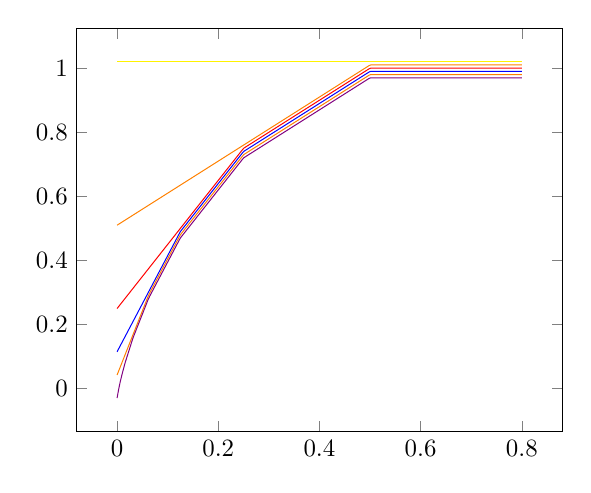
\begin{tikzpicture}[scale=0.9]
\begin{axis}[samples=250]
\addplot[yellow,domain=0:0.8] {1+0.02};

\addplot[orange,domain=0:0.8] {min(x+1/2, 1)+0.01};


\addplot[red,domain=0:0.8] {min(2*x+1/4, x+1/2, 1};
\addplot[blue,domain=0:0.8] {min(3*x+1/8,2*x+1/4, x+1/2, 1)-0.01};
\addplot[orange,domain=0:0.8] {min(4*x+1/16,3*x+1/8,2*x+1/4, x+1/2, 1)-0.02};

\addplot[violet,domain=0:0.8] {min(
10*x+1/1424,
9*x+1/712,
8*x+1/356,
7*x+1/128,
6*x+1/64,
5*x+1/32,
4*x+1/16,3*x+1/8,2*x+1/4, x+1/2, 1)-.03};


\end{axis}

\end{tikzpicture}
\caption{\small Tropical polynomials $\varphi_0,\dots,\varphi_4$ (top to bottom), and the limit tLs $\varphi$ (in violet). The points where the slope changes are  the tropical roots of $\varphi$, i.e.~the points $x=2^{-(i+1)}$, satisfying $ix+2^{-i}=(i+1)x+2^{-(i+1)}$.}
\label{fig:plot1}%\end{figure}%
\end{wrapfigure} %%

A \emph{tropical root} of a tropical polynomials $\varphi$ is a point $x\in \Lawv$ where $\varphi$ is not differentiable. In other words, the roots of $\varphi$ are the points where the minimum defining $\varphi$ is attained at least twice (i.e.~where the slope of $\varphi$ changes).
For instance, the tropical roots of $\varphi_{n+1}$ are of the form $2^{-(i+1)}$, for $0\leq i \leq n$.
Tropical roots yield the usual factorization property of roots: if $x_{0}$ is a root of $f$, this factorizes as
$f(x)=\min\{x,x_{0}\}+ g(x)$. Yet, unlike in standard algebra, tropical roots can be computed in linear time \cite{Noferini2015}.
%Tropical polynomials and their roots are the main object of study of tropical geometry.
%
%A
% simple calculation shows that this condition corresponds, in the tropical setting, to the usual notion of root. 

A \emph{tropical Laurent series} of one variable is a function $f:\Lawv\to\Lawv$ of shape $f(x)=\inf_{n\in\N}\{nx+\matr f_{n}\}$, with $\matr  f_{n}\in\Lawv$.
In other words, it is a ``limit'' of tropical polynomials of higher and higher degree.
E.g., the tLs $\varphi(x):=\inf_{n\in\N}\set{nx+2^{-n}}$ (see Fig.~\ref{fig:plot1}), that we will take as our running example, 
is the ``limit'' of the polynomials $\varphi_{n}$.
Since $\inf$s are not in general $\min$s, the behaviour of tLS may be less predictable than that of tropical polynomials~\cite{Porzio2021}. %For instance, tropical roots for tLs (see \cite{Porzio2021}) may also include limit points of their domain.

%
%
%We will take as our running example
%%given respectively by Equation~\ref{eq:polytrop} and Equation~\ref{eq:defTLS}.
%A positive $x\in[0,\infty)$ is said to be a (finite) \emph{tropical root} of a tropical Laurent series $f:\Lawv\to\Lawv$ iff $f$ is not differentiable at $x$ (w.r.t.\ the usual topology on $\BB R_{\geq0}$.This is equivalent to ask that the $\inf$ defining $f$ at $x$ is obtained \emph{at least} twice.{\color{red} \`e vero anche per TLS o solo per poly questo? Inoltre, Robol parla anche di finite end-points of the domain: nel nostro caso sarebbe $x=0$}

%\begin{example}\label{ex:famous_ex}
% The function $f:\Lawv\to\Lawv$ defined by $f(x):=\inf\limits_{n\in\N}\set{nx+\frac{1}{2^n}}$ is a tropical Laurent series.
%\end{example}

%By plotting its graph {\color{red}vogliamo plottarlo?}, we observe several properties that we will lift to the more general case that we will consider in the next lines, and this example will serve as running one.

%\begin{remark}%[Tropical Laurent series]
 Remark that the map $t^!:\Lawv^X\to\Lawv^Y$ introduced above from a matrix $t\in\HOM{\LREL_!}{X}{Y}$, corresponds to a tLs with \emph{possibly infinitely} many variables (in fact, as many as the elements of $X$). %In the following we will also refer to them as tLs. 
% We will call them simply \emph{tropical Laurent series (tLs)}.
% %Since in the general case of $\QREL$, $t^!$ is a Laurent series with operations in $Q$, let us call \emph{tropical Laurent series} the functions of shape $t^!$ for some $t\in\HOM{\LREL_!}{X}{Y}$.
%\end{remark}
%
%We find the usual notion of tLs of one variable as follows:
%\begin{remark}
By identifying $!\set{*}\simeq \N$ and $\Lawv^{\set{*}}\simeq\Lawv$, the tLs generated by the morphisms in $\HOM{\LREL_!}{\set{*}}{\set{*}}$ are exactly the %functions $f:\Lawv\to\Lawv$ of shape $f(x)=\inf_{n\in\N}\set{nx+\matr f(n)}$, for some $\matr f:\N\to\Lawv$, i.e.\ we recover the 
usual tLs's of one variable.
% \end{remark}
 \begin{remark}
 Our running example is indeed of shape $\varphi=t^!$, for $t\in\Lawv^{!\set{*}\times\set{*}}$, $t_{\mu,*}:=2^{-\# \mu}$.
 However, it is not the interpretation of a $\lam$-term, because its matrix $t$ is not discrete.
% Therefore $\LREL_!$ is not a full-complete model of $\STLC$.
\end{remark}



 In a similar way, tLs
$f:\Lawv^X\to\Lawv^Y$ 
 with \emph{finite} supports $\C F_b=\set{\mu\in!X\mid\matr f_{\mu,b}\neq\infty}$, and which have thus shape $f(x)_b=\min_{\mu\in\C F} \set{\mu x+ t_{\mu,b}}$, are generalisation of usual tropical polynomials to the case of possibly infinitely many variables.
For instance, for a $t\in\HOM{\LREL}{!_n X}{Y}$ (this is in particular the case for the interpretations of $\BSTLC$-terms), we will consider the (generalised) tropical polynomial $t^!:\Lawv^X\to\Lawv^Y$ defined by $t^!(x)_b:=\inf_{\mu\in !_nX}\{\mu x+t_{\mu,b}\}$.
% 
% , i.e.~for a \emph{finite} set $\C F\subseteq \, !X$.
%%Remark that we also find usual \emph{tropical polynomials} of tropical geometry as a particular case: they 
%correspond to the tLs for which the support $\set{n\in\N\mid\widehat f(n)\neq\infty}$ of $\widehat f$ is \emph{finite}. 
%Actually, for us \emph{tropical polynomial} will mean a function 
%\end{remark}

Looking at Fig~\ref{fig:plot1}, we see that $\varphi$, just like the polynomials $\varphi_{n}$, is non-decreasing and concave.
This is indeed always the case:

\begin{proposition}\label{prop:nondecr+conc}
 Any tLs $f:\Lawv^X\to\Lawv^Y$ is non-decreasing and concave, w.r.t.\ the pointwise order.
\end{proposition}

%In Example~\ref{ex:famous_ex}, 
Again by looking at Fig~\ref{fig:plot1} it appears that, \emph{far from $0$}, $\varphi$ behaves like some polynomials $\varphi_{n}$.
In particular, %for all $\epsilon >0$, $f$ coincides on $[\epsilon,\infty]$ with some polynomial $\varphi_{n}$. More, precisely, 
$\varphi$ coincides on $[\epsilon,\infty]$ with $\varphi_{n}$,
for $\epsilon \geq 2^{-(n+1)}$ (the smallest tropical root of $\varphi_{n}$).
However, at
%
%$x\in [\epsilon,\infty]$, with $\epsilon>0$
%It can be proven by hand that $\varphi(x)$ is a $\min$ for all $x>0$.
 $x=0$ we have that $\varphi(x=0)=\inf_{n\in\N} 2^{-n}=0$, and this is the only point where the $\inf$ is \emph{not} a $\min$.
Also, while the derivative of $f$ is bounded on all $(0,\infty)$, for $x\to 0^+$ it tends to $\infty$.
This phenomenon is reminiscent of \cite[Example 7]{Ehrhard2005},
%Differentials and Distances in Probabilistic Coherence Spaces. FSCD 2019
which actually motivated our first investigations.
In fact, this behaviour is shared by all tLs with \emph{finitely} many variables, as shown by the following result (we identify $!\set{1,\dots,k}\simeq \N^k$, so the matrix of a tLs $f$ with finitely many variables $x=x_1,\dots,x_k$ (and one output variable) is given as a $\matr f:\N^k\to\Lawv$, $f$ having shape $f(x)=\inf_{n\in \N^k}\set{nx+\matr f(n)}$, with $nx$ the scalar product).

\begin{theorem}\label{theorem:fepsilon}
 Let $k\in\N$ and $f:\Lawv^k\to\Lawv$ a tLs with matrix $\matr f:\N^k\to\Lawv$.
 For all $0<\epsilon<\infty$, there is a \emph{finite} $\C F_\epsilon \subseteq \N^k$ such that 
% 
% \begin{enumerate}
%  \item If $\C F_\epsilon=\emptyset$ then $f=\infty$ on all $\Lawv^k$;
%  \item If $f(x_0)=\infty$ for some $x_0\in[0,\infty)^k$, then $\C F_\epsilon=\emptyset$;
  %\item 
$f$ coincides on all $[\epsilon,\infty]^k$ with the tropical \emph{polynomial} $P_\epsilon(x):=\min_{n\in \C F_\epsilon}\set{nx+\matr f(n)}$.
% \end{enumerate}
\end{theorem}
\begin{proof}[Proof sketch]
Let $\C F_\epsilon$ be the set of $n\in\N^{k}$ such that 
$\widehat f(n)<\infty$ and $\widehat f(m)> \widehat f(n)+\epsilon$ holds for all $m\prec n$, where $\preceq$ is the pointwise order on $\N^k$.
The core of the proof is showing that this set is indeed finite and enough for computing $f$.
\end{proof}




\subsection{Continuity of tLs}\label{subsec:cont}%$\Lawv^{X}$ as a normed cone}

The tLs $\varphi$ is continuous on $\BB R_{\geq0}$ (w.r.t.\ the usual norm of real numbers).
By considering the usual norm $\norm{x}_\infty:=\sup_{a\in X} \absv{x_a}$ on $\Lawv^X$, we can generalise this property by dropping the case of $x$ having some $0$ coordinate:

\begin{theorem}\label{thm:cont}
 All tLs $f:\Lawv^X\to\Lawv$ are continuous on $\BB R_{>0}^X$, w.r.t.\ to the norm $\norm{\cdot}_\infty$.
\end{theorem}
\begin{proof}
 It follows after adapting [Proposition 4.4, \cite{Cobzas2017}] in order to prove that if a real-valued function on a locally convex topological $\BB R$-vector space is, locally around $x$, concave and bounded by a finite constant, then it is continuous at $x$.
\end{proof}

We conclude this subsection by noticing that $\Lawv^X$ with the usual $+$ and the usual $\cdot$ is a $\BB R_{\geq0}$-semimodule.
Together with the norm $\norm{\cdot}_\infty$, it can be proved that it is a Scott-complete \emph{normed cone} (see~\cite{Selinger2004}, or the appendix, for such notions).
Its cone structure induces an order on it, called its \emph{cone order}:
$x\leq y$ iff $y=x+z$ for some (unique) $z\in\Lawv^X$.
Such order actually coincides with the pointwise order on $\Lawv^X$.
This makes it a Scott-continuous dcpo.
Suitable categories of cones have been recently investigated as models of probabilistic computation (\cite{Crubillie2018, EhrPagTas2018, Ehrhard2020}).
Here we will just mention that:

\begin{theorem}\label{thm:ScottCont}
 All monotone (w.r.t.\ pointwise order) and $\norm{\cdot}_{\infty}$-continuous functions $f:(0,\infty)^X\to (0,\infty)$ are Scott-continuous.
 In particular, all tLs $f:\Lawv^X\to\Lawv$ are Scott-continuous on $(0,\infty)^X$ w.r.t.\ the pointwise orders.
\end{theorem}
\begin{proof}
 Use the fact, taken from \cite{Selinger2004}, that in a normed $\R_{\geq 0}$-cone $P$, considered with its cone-order, if every bounded directed net in $P$ admits a sup, and if $(v_i)_{i\in I}$ is a directed net in $P$ with an upper bound $v\in P$, then $\exists\bigvee_{i\in I} v_i \in P$ and, if $\inf_{i\in I} \norm{v-v_i} =0$, one has $\bigvee_{i\in I} v_i = v$.
\end{proof}



\subsection{Lipschitz-continuity of tLs}\label{sec:4C}%$\Lawv^{X}$ as a metric space.}


%The norm $\norm{\cdot}_\infty$ naturally induces a metric $\norm{x-y}_{\infty}$ over the spaces $\Lawv^{X}$.
We will show that tLs satisfy suitable Lipschitz properties w.r.t.\ $\norm{\cdot}_\infty$. 

Let us first look at tropical linear functions:


\begin{proposition}\label{prop:troplinear}
All tropical \emph{linear} functions $f: \Lawv^{X}\to \Lawv^{Y}$ are non-expansive.  
\end{proposition}
%\begin{proof}[Proof sketch]
%Using the fact that $f(\B x)_{b}= \inf_{a\in X}\matr f_{a,b}+\B x_{a}$,
%the problem reduces to checking that $|(\matr f_{a,b}-\B x_{a})- (\matr f_{a,b}-\B y_{a})| = |\B x_{a}-\B y_{a}|\leq \| \B x-\B y\|_{\infty}$.\end{proof}
This result shows that, in analogy with that happens in usual metric semantics, linear programs are interpreted by non-expansive functions. 
%\begin{proof}
%Using $f(\B x)_{b}= \inf_{a\in X}\matr f_{a,b}+\B x_{a}$,
%first observe that $|(\matr f_{a,b}-\B x_{a})- (\matr f_{a,b}-\B y_{a})| = |\B x_{a}-\B y_{a}|\leq \| \B x-\B y\|_{\infty}$; we now have
%$|f(\B x)_{b}-f(\B y)_{b}| \leq |(\inf_{a\in X}\matr f_{a,b}-\B x_{a})-(\inf_{a\in X}\matr f_{a,b}-\B y_{a})| \leq
%\sup_{a\in X}|(\matr f_{a,b}-\B x_{a})- (\matr f_{a,b}-\B y_{a})|\leq 
% \| \B x-\B y\|_{\infty}$.
%\end{proof}

%Before looking at what happens in the case of non-linear programs, let us make the metric structure of $\LREL$ explicit. 
The following proposition provides a useful characterization of the functional metrics in $\LREL$, relying on 
the bijection between $\HOM{\LREL}{X}{Y}$ and set of tropical linear functions from $\Lawv^{X}$ to $\Lawv^{Y}$.

\begin{proposition}
For all tropical linear functions $f,g:\Lawv^{X}\to \Lawv^{Y}$, $d_{\infty}(\matr f,\matr g)=d_\infty(f,g)$.% $\norm{ \matr f-\matr g}_{\infty} =  \sup_{x\in \Lawv^{X}} \norm{ f( x)-g(x)}_{\infty}$.
\end{proposition}

Let us now consider the case of bounded exponentials:
\begin{proposition}\label{prop:boundedlip}
If a tLs $f: \Lawv^{X}\to \Lawv^{Y}$ arises from a matrix $\matr f:!_{n}X\times Y\to \Lawv$, then $f$ is $n$-Lipschitz-continuous.
\end{proposition}
\begin{proof}[Proof sketch]
This follows from Proposition \ref{prop:troplinear} and the remark that, for all $x\in \Lawv^{X}$, $\norm{ !_{n} x-!_{n} y}_{\infty}\leq n\cdot \norm{ x- y}_{\infty}$, where $!_{n} x$ is the restriction of $! x$ to $\C M_{\leq n}(X)$.%
%Using the fact that $f(\B x)_{b}=\inf_{\mu\in \C M_{\leq n}(X)}\{ \matr f_{\mu,b}+ \mu (!_{n}\B x) \}$, where $!_{n}\B x\in \Lawv^{\C M_{\leq n}(X)}$ is given by 
%$(!_{n}\B x)_{[a_{1},\dots, a_{k}]}=\sum_{i=1}^{k}\B x_{a_{i}}$, 
%it suffices to check that $\| (!_{n}\B x)-(!_{n}\B y)\|_{\infty}\leq n\cdot \| \B x-\B y\|_{\infty}$ and apply Proposition \ref{prop:troplinear}.
\end{proof}
This result is perfectly analogous to what happens in the metric models discussed in Section \ref{section2}, the bounded exponentials $!_{n}$ playing the role of the re-scaling trick.

Observe that, for any tropical polynomial $\varphi:\Lawv^{X}\to \Lawv^{Y}$, the associated matrix has shape $!_{\mathrm{deg}(\varphi)}(X)\times Y\to \Lawv$ (as a monomial $\mu_ix+c_{i}$ yields a matrix entry on $!_{\#\mu_i}X\times Y$). Hence, using Proposition \ref{prop:boundedlip}, we have:
\begin{corollary}\label{prop:polylip}
For any tropical polynomial $\varphi:\Lawv^{X}\to\Lawv$, $\varphi$ is $\mathrm{deg}(\varphi)$-Lipschitz continuous.
\end{corollary}

Let us now look at what happens with tLs, i.e.~when considering the full exponential $!$.
As consequence of Theorem~\ref{theorem:fepsilon}, the tLs with \emph{finitely many} variables are always \emph{locally} Lipschitz on all $\BB R_{>0}$.
Actually, we can prove a more general statement, also covering the infinitary case.


\begin{theorem}\label{thmTLSlocLip}
 All tLs $\Lawv^X\to\Lawv$ are locally Lipschitz on $\BB R_{>0}^X$.
\end{theorem}
\begin{proof}[Proof sketch]
The core of the proof is a convex analysis argument (see the Appendix) showing that an arbitrary function $f:\Lawv^X\to\Lawv$ which is non-decreasing, concave and continuous, must be locally Lipschitz. 
\end{proof}


Finally, let us discuss the differential structure. The differential operator $D$ of $\LREL_{!}$ translates into a differential operator $D_{!}$ turing a tLs $f:\Lawv^{X}\to \Lawv^{Y}$ into a tLs $D_{!}f:\Lawv^{X}\times \Lawv^{X}\to \Lawv^{Y}$, linear in its first variable, and given by 
\begin{equation}
D_{!}f(x,y)_{b}=\inf_{a\in X, \mu\in !X}\left\{\matr f_{\mu+a}+x_{a}+\mu y\right\}
\end{equation}
One can check that, when $f$ is a tropical polynomial, $D_{!}f$ coincides with the standard tropical derivative (see e.g.~\cite{Grigoriev2017}).
Moreover, the Taylor formula \eqref{eq:taylorcat} yields a ``tropical'' Taylor formula for tLs of the form 
\begin{equation}
f(x)=\inf_{n}\left\{D_{!}^{(n)}(f)(!_{n}x,\infty)\right\}
\end{equation}
The following result shows that the distance between two tropical maps can be approximated using the terms appearing in their Taylor expansions:
\begin{proposition}
For all tLs $f,g: \Lawv^{X}\to \Lawv^{Y}$, and for all $n\in \BB N$, 
the functions $x\mapsto D_{!}^{(n)}(f)(!_{n}x,\infty)$ are $n$-Lipschitz. Moreover 
$\norm{ \matr f-\matr g}_{\infty}= \sup_{n} \norm{ {\delta^{(n)}f}- {\delta^{(n)}g}}_{\infty}$, 
where $\delta^{(n)}h$ indicates the matrix of $D_{!}^{(n)}h$.
%where $\delta^{(n)}f:( \Lawv^{X})^{n}\to \Lawv^{X}$ is the tropical linear function $\delta^{(n)}f(\B x_{1},\dots, \B x_{n})=
%(\Der^{(n)}f)(\B x_{1},\dots, \B x_{n}, \infty)$. 
\end{proposition} 


The results just presented translate into the following facts about the interpretation of higher-order programs:

\begin{corollary}
Let $\model A$ be a finite set.
\begin{enumerate}
\item $\model{\Gamma \vdash_{\BSTLC} M:A}^!:\Lawv^{\model\Gamma} \to \Lawv^{\model A}$ is a \emph{tropical polynomial}, thus (as $\model A$ is finite), a \emph{Lipschitz} function.
\item $\model{\Gamma \vdash_{\STLC} M:A}^!:\Lawv^{\model\Gamma} \to \Lawv^{\model A}$ is a \emph{locally} Lipschitz map.
\item $\Te{M}$ decomposes $\model{\Gamma \vdash_{\STLC} M:A}^!$ as an $\inf_{t\in\Te{M}}\model{\Gamma\vdash_{\STDLC} t:A}^!$ of \emph{tropical polynomials}, thus (as $\model A$ is finite), \emph{Lipschitz} functions.
\end{enumerate}
\end{corollary} 
\begin{proof}
1). We already observed that the interpretation of a $\BSTLC$-type $B$ is alway a finite set, so thus is $!_n \model B$.
So the $\inf$ defining $(\_)^!$ is actually a $\min$.
So the interpretation of a bounded term is a tropical polynomial, so we apply Corollary~\ref{prop:polylip} to each coordinate of the image, and since $\model A$ is finite (by taking the maximum Lipschitz constant among the finite number of them), we obtain the thesis.
2). It follows immediately from Theorem~\ref{thmTLSlocLip} and the fact that $\model A$ is finite.
3). It follows from \autoref{cor:T(M)=M} plus the easily checked fact that, for $(f_n)_{n\in\N}\subseteq\Lawv^{!X\times Y}$, we have $\left(\inf_{n\in\N} f_n\right)^!:\Lawv^X\to\Lawv^Y$, with $\left(\inf_{n\in\N} f_n\right)^!=\inf_{n\in\N} f_n^!$.
\end{proof}

Remark that the restriction $\model A$ finite is without loss of generality, since by Currying all programs can be seen having type $*$, which is natural to interpret as a singleton.

A consequence of (3) is that the distance between two programs can always be approximated via Lipschitz tropical polynomial approximants of the initial two programs.
\begin{corollary}
 Let $\Gamma \vdash_{\STLC} M:A$ and $\Delta\vdash_{\STLC} N:B$.
 For all $\epsilon>0$, $x\in\Lawv^{\model \Gamma}$, $b\in\model A$, there exist $t\in\Te{M}$, $u\in\Te{N}$ s.t.\ $\big| \model{\Gamma \vdash_{\STLC} M:A}^!(x)_b - \model{\Delta \vdash_{\STLC} N:B}^!(x)_b \big| \leq 2\epsilon + \big| \model{\Gamma \vdash_{\STDLC} t:A}^!(x)_b - \model{\Delta \vdash_{\STDLC} u:B}^!(x)_b \big|$.
\end{corollary}

\begin{remark}
 Let $X$, $Y$ be sets and let $\langle \_,\_\rangle:X\times Y \to \mathbb{R}$.
 For $f:X\to \mathbb R$, define $f^*:Y\to \mathbb R$ by $f^*(y):= \sup_{x\in X}\{\langle x,y\rangle - f(x)\}$.
 Then for $X=!A$, $Y=\Lawv^A$, where $A$ is a set, and $\langle \mu, y \rangle:= \mu y$, we have that $f^!=(-f)^*$ for all $f\in\Lawv^{!A}$.
 This is precisely the same formal construction yielding the well-known convex conjugate $f^*$ of a function $f$, by taking $X$ any vector space, $Y$ its dual space, and $\langle \_,\_\rangle$ the application bilinear form (acting as the scalar product on coordinates).
 This construction is in turn a generalisation of the Legendre transformation.
 Despite the formal constructions being the same, we ignore for the moment if these could be connected to the study of high-order programs in our setting.
\end{remark}



\section{Lipschitz Meets Taylor}\label{sec:TayLip}
% !TEX root = /Users/paolopistone/Documents/GitHub/tropicalnew/CSL24/main.tex


We now have all elements necessary to relate the metric and differential analysis of higher-order programs in the tropical relational model. 

The key ingredient is the notion of Taylor expansion $\Te{M}$ of a $\lambda$-term $M$, which is a set of terms of the differential $\lambda$-calculus defined as follows:
%
%
%
% which is defined as follows: 
%
%that we now quickly recall. 
%
%
%Let $M\langle N_{1},\dots, N_{k}\rangle$ be an abbreviation for
%$\mathsf D^{k}[M, N_{1},\dots, N_{k}]0$. A \emph{resource $\lambda$-term} is any term belonging to the grammar $t::= x \mid \lambda x.t \mid t \langle t,\dots, t\rangle$.
%%
%
%The Taylor expansion of a $\lambda$-term is a set of resource terms $\Te{M}$ defined inductively as 
%
$\Te{x}=\{x\}$, $\Te{\lambda x.M}=\{\lambda x.t\mid t\in \Te{M}\}$ and 
$\Te{MN}=\{t\cdot \langle u_{1},\dots, u_{k}\rangle  \mid k\in \mathbb N, t\in \Te{M}, u_{i}\in \Te{N} \}$, where $t\cdot \langle u_{1},\dots, u_{k}\rangle$ is an abbreviation for $\mathsf D^{k}[t, u_{1},\dots, u_{k}] 0$. 
Observe that in the terms appearing in $\Te{M}$ all applications are always \emph{bounded}: they may use an exact number of copies of their input. 
Such terms are usually called \emph{resource $\lambda$-terms} \cite{Pagani2009, Manzo2012}.
Considering the term $M=zxx$ from Example \ref{ex:zxx}, all terms
 $t_{n,m}=z \,\langle x^{n}\rangle\,\langle x^{m}\rangle$, for $n,m\in \mathbb N$, are in $\Te{M}$. 
Observe that the interpretation of $t_{n,m}$ yields a tropical polynomial
$\model{t_{n,m}}^{!}(x)(z)= y_{[n,m]}+(n+m)x$, rather than a tps. 
However, resource $\lambda$-terms need not always yield a tropical polynomial. For instance, consider $y:(*\to*)\to (*\to*), x:(*\to *) \vdash t:  (*\to  *)$
with $t=y\cdot \langle y\cdot \langle x\rangle \rangle\in \Te{y(yx)}$. Then 
$\model{t}^{!}: \Lawv^{  \mathcal M_{\mathrm{fin}}(\mathbb N)\times \mathbb N}
\times \Lawv^{\mathbb N} \to \Lawv^{\mathbb N}$ is given by
$
\model{t}^{!}(y,x)_{i}= \inf_{m,n\in \mathbb N}\big\{    y_{[m],i}  +  y_{[n],m}+  x_{n}\}
$, 
which is not a polynomial. Yet, $\model{t}^{!}$ is Lipschitz, more precisely, 1-Lipschitz in $x$ and 2-Lipschitz in $y$. This is a general fact, as shown below.

%
%$\Te{MN}$ of $MN$ is the set $\set{\Der^{n}[t,u_1,\dots,u_n]0 \mid n\in\N,t\in\Te{M},u_i\in\Te{N}}$.
We have already shown that the tropical differential makes $\LREL_{!}$ a model of the differential $\lambda$-calculus. We now show that it also models the Taylor expansion (this needs not be true for \emph{any} CC$\partial\lambda$C).
First, it can be patiently checked that in $(\LREL_!,D)$ all morphisms can be Taylor expanded  (see \cite[Definition 4.22]{Manzo2012}):

\begin{theorem}\label{thm:modelsTaylor}
 For all $t\in\HOM{\LREL_!}{Z}{!X\multimap Y}$, $s\in\HOM{\LREL_!}{Z}{X}$ we have:%, the evaluation of $t$ over $s$ yields 
 \begin{align}\label{eq:taylorcat}
  \RM{ev}\circ_!\langle t,s\rangle =
  \inf\limits_{n\in\N}
  \set{((\dots((\Lambda^- t)\star s)\star \dots)\star s)\circ_! \langle \RM{id},\infty \rangle}.
 \end{align} 
\end{theorem}
%It is worth discussing the formula above a bit more. 
The equation above is a nothing more than a tropical version of the Taylor formula from the Introduction:
%:\HOM{\LREL}{!Z}{X\multimap Y}\to \HOM{\LREL}{!(Z+X)}{Y}$
%$\star:\HOM{\LREL}{!(Z+X)}{Y}\times\HOM{\LREL}{!Z}{X}\to \HOM{\LREL}{!(Z+X)}{Y}$ is defined as 
$u\star s= (Du)\circ_{!} \langle \langle  \infty, s\circ_{!} \pi_{1}\rangle,\mathrm{id}\rangle$ corresponds to the application of the derivative of $u$ on $s$, and $\Lambda^-$ is the uncurry operator.
Hence the right-hand term in \eqref{eq:taylorcat} corresponds to the $\inf$ of the $n$-th derivative of $\Lambda^{-}t$ applied to ``$n$ copies'' of $s$.
%,  i.e.~it coincides with the tropical %interpretation of the
%version of the usual Taylor expansion.
%Moreover, since $\LREL_!$ has countable sums (all $\inf$'s converge), and thanks to equation \eqref{eq:taylorcat}, an immediate adaptation of the proof of [Theorem 4.23, \cite{Manzo2012}] entails that the interpretation of the $\STDLC$-Taylor expansion of a $\STLC$-term $M$ given in \eqref{eq:taylor}, converges to the interpretation of $M$.


Second, since $\LREL_!$ has countable sums (all countable $\inf$s converge), an immediate adaptation of the proof of \cite[Theorem 4.23]{Manzo2012} shows:

\begin{corollary}\label{cor:T(M)=M}
 %For $\Gamma\vdash_{\STLC} M:A$, we have %$\model{\Gamma\vdash_{\STDLC} \Te M:A}:=
$\model{\Gamma\vdash_{\STLC} M:A}=\inf_{t\in\Te{M}} \model{\Gamma\vdash_{\STDLC} t:A}$. %the interpretation of the Taylor expansion of a $\STLC$-term $M$, given in \eqref{eq:taylor}, converges to the one of $M$.
\end{corollary}




Using the results of the previous section, as well as the results above, we can deduce the following properties:

\begin{theorem}\label{thm:taylor}
Let $\mathcal S$ be one of $\RM{PCF}^{\Lawv},\STLC,\BSTLC,\STDLC$. Let $\Gamma\vdash_{\mathcal S}M:A$ and $a\in \model{A}$.
\begin{enumerate}
\item For $\mathcal S=\BSTLC$, $\model{\Gamma\vdash_{\mathcal S}M:A}^{!}_{a}$ is a tropical polynomial, and thus Lipschitz;

\item For $\mathcal S=\STDLC$, if $t\in \Te{M}$, then $\model{\Gamma\vdash_{\mathcal S}t:A}^{!}_{a}$ is Lipschitz;

\item For $\mathcal S=\STLC,\RM{PCF}^{\Lawv}$, then $\model{\Gamma\vdash_{\mathcal S}M:A}^{!}_{a}$ is locally Lipschitz;

\item For $\mathcal S=\STLC$, $\Te{M}$ decomposes $\model{\Gamma \vdash_{\STLC} M:A}^!_{a}$ as an $\inf_{t\in\Te{M}}\model{\Gamma\vdash_{\STDLC} t:A}^!_{a}$ of {Lipschitz} functions.
\end{enumerate}

\end{theorem}
\begin{proof}
1). As we already observed, the interpretation of a bounded term is a tropical polynomial.
2.) From Proposition \ref{prop:troplinear} 2.~observing that a resource term $t(x)$ may use a variable $x$ a fixed number $n$ times, so that its matrix lies in $\Lawv^{!_{n}X\times Y}$. 
%Now we apply Corollary~\ref{prop:polylip} to each coordinate of the image, and by taking the maximum Lipschitz constant among the finite number $\mathrm{Card}(\model A)$ of them, we obtain the thesis.
3). From Theorem~\ref{thmTLSlocLip}.
4). It follows from \autoref{cor:T(M)=M} plus the fact that, for $(f_n)_{n\in\N}\subseteq\Lawv^{!X\times Y}$, we have $\left(\inf_{n\in\N} f_n\right)^!:\Lawv^X\to\Lawv^Y$, with $\left(\inf_{n\in\N} f_n\right)^!=\inf_{n\in\N} f_n^!$.
\end{proof}




%
%From this we deduce, inductively, the following fact:
%\begin{proposition}
%For any resource $\lambda$-term $t$, if $\Gamma\vdash_{\STDLC}t:A$, then $\model{\Gamma\vdash_{\STDLC}t:A}^{!}$ is a Lipschitz function.
%\end{proposition}
%
%
%This result shows that the interpretation of a program can be approximated via a family of tropical polynomials, and leads to.
% \begin{theorem}\label{thm:taylor}
% $\Te{M}$ decomposes $\model{\Gamma \vdash_{\STLC} M:A}^!_{a}$ as an $\inf_{t\in\Te{M}}\model{\Gamma\vdash_{\STDLC} t:A}^!_{a}$ of \emph{tropical polynomials}, that is,of \emph{Lipschitz} functions.
%\end{theorem}


We conclude our discussion with an application of the Taylor expansion in $\LREL_{!}$: as proved in the previous section, all tps are locally Lipschitz; now, Theorem \ref{thm:taylor} can be used to compute approximations of the Lipschitz constants of an actual higher-order program.

\begin{corollary}
Suppose $x: A \vdash_{\STLC}M:B$ and $\vdash_{\STLC} N:A$. 
Then for all $t\in \Te{M}$ such that $\model{t}^{!}(\model{N})\neq \infty$, and $\delta>0$, the tps $\model{ x:A\vdash_{\STLC}M:B}^{!}$ is $\frac{\model{t}^{!}(\model{N}+2\delta)}{\delta}$-Lipschitz over the open ball
 $B_{\delta}(\model{N})$.
\end{corollary}
\begin{proof}
We apply the Lipschitz estimate from Thm.~\ref{thmTLSlocLip} for $\model{M}^{!}$,  and use the fact that, from Thm.~\ref{thm:taylor} 4.~it follows that $\model{t}^{!}\geq \model{M}^{!}$.
To conclude, since $\model{t}^{!}$ is concave and non-decreasing, $\max_{\overline{B_{3\delta}(x)}}\model{t}^{!}= \model{t}^{!}(x+3\delta)$, which yields the stated Lipschitz estimate. 
\end{proof}
%{\color{red}ADD PROOF SKETCH}

\begin{example}
Consider again the term $M=zxx$ from Example \ref{ex:zxx}-
%, satisfying $x:*, z:(*\to*\to*) \vdash M:  *$. Since $\mathcal M_{\mathrm{fin}}(\{*\})\simeq \mathbb N$, we have that 
%
% $\model{M}^{!}: \Lawv \times \Lawv^{\mathcal M_{\mathrm{fin}}(\mathbb N\times \mathbb N)}\to \Lawv$ is given by
 The (generalized) tps $\model{M}^{!}(x)(y)= \inf_{n,n'\in \mathbb N}\{y_{[(n,n')]}+(n+n')x\}$ is not (globally) Lipschitz: for any 
$L>0$, choose a natural number $N>L$, let $Y\in \Lawv^{\mathcal M_{\mathrm{fin}}(\mathbb N\times \mathbb N)}$ be such that $Y_{\mu}<\infty$ only if $\mu=[(n,n')]$ with $n+n'\geq N$; then $|\model{M}^{!}(x)(Y)- \model{M}^{!}(x+\epsilon)(Y)|\geq N\epsilon > L\epsilon$. 
Now take the approximant $t= z \langle x^{N-1}\rangle \langle x\rangle \in \Te{M}$ (chosen so that $\model t^{!}(x)(Y)<\infty$). Its interpretation is the monomial 
$\model{t}^{!}(x)(Y) = Y_{[(N-1,1)]}+Nx$. We can then compute a Lipschitz-constant for $\model{M}^{!}$ around $\langle x,Y\rangle$
as $\frac{1}{\delta}\model{t}^{!}(\langle x,Y\rangle+\delta)= 3N+3 + \frac{Y_{[(N-1,1)]}+Nx}{\delta}$. 
\end{example}
%    
%    %
%  Consider now $F\in \Lawv^{\mathcal M_{\mathrm{fin}}(\mathbb N\times \mathbb N)}$ given by $F_{\mu}=0$ if $\mu=[(1,1)]$ and $F_{\mu}=\infty$ otherwise. 
%  Then $\model{M}^{!}(\langle x,F\rangle)=2x$
%%We show that we can compute a local 
%More formally, the differential operator $\Der[-]$ transforms a function $M:A\to B$ into a function $\Der[M]: A\to (A\to B)$ which is linear in its first argument. 
%Since $M$ may rather ask for several copies of $N$, this requires a form of non-determinism: 
%For example, if $M$ is the term $\lambda fx.f(fx)$ considered before, $\Der[M]$ takes a first input $N$ and passes it linearly to $M$. Notice that there are two ways of doing so, corresponding to the two bound occurrences of $f$ in $M$: either by applying $N$ to $fx$, or by 
%applying $f$ linearly to $Nx$ (indeed, if $f$ were applied in an unrestricted way, it might duplicate $Nx$, so that $N$ would not be used linearly). This justifies the equation below, in which $\Der[M]$ is identified with the non-deterministic sum of the two possible linear choices:
%\begin{align}
%\Der\left[\lambda f x.f(fx)\right]\cdot N = 
%\lambda fx. N(fx) + \left(\Der[f]\cdot (Nx)\right)(fx)
%\end{align}
%More generally, one can define a notion of $k$-bounded application $\Der^{(k)}[M]\cdot N^{k}$, where $\Der^{(0)}[M]\cdot N^{0}= M$ and $\Der^{(k+1)}[M]\cdot N^{k+1}= \Der[ \Der^{(k)}[M]\cdot N^{k}]\cdot N$, corresponding to passing $N$ to $M$ exactly $k$ times.
%
%
%The name ``differential'' for the operator $\Der[-]$ is justified by the fact that it satisfies many properties of the usual differential operator of analysis $\Der[f]:= \lambda xy. \frac{\mathsf df(y)}{\mathsf dy}\cdot x$. Notably, it is additive in its first variable (i.e.~it commutes with the non-deterministic sum operator), and satisfies the chain rule.
%Most famously, the differential operator can be used to define a Taylor formula for $\lambda$-terms, which decomposes an unrestricted application into a formal non-deterministic sum of bounded applications:

%
%More generally, the relational semantics interprets unbounded programs as \emph{analytic functions}, that is, as functions admitting a representation as power series. For instance, observing that an analytic map $f: \BB R\to \BB R$, where $f(x)=\sum_{n}\widehat f_{n}\cdot x^{n}$ is uniquely determined by the sequence $\widehat f_{n}$, the program $M_{\infty}:=\lambda fx.fx: (\BB R\To \BB R)\To (\BB R\To \BB R)$ is represented by the power series below:
%\begin{align}
%F_{\infty}(f,x)= \sum_{n=0}^{\infty} \widehat f_{n} x^{n}
%\end{align}
%By restricting ourselves to bounded applications, the terms in the power series become finite, that is, the interpretation becomes a \emph{polynomial}: for instance, the program $M_{2}:=\lambda fx. \sum_{i=0}^{2}\Der^{(i)}[f]\cdot x^{i}$, corresponding to passing $x$ \emph{at most twice} to $f$, is represented by the polynomial
%\begin{align}
%F_{\leq 2}(f,x)=\widehat f_{2} x^{2}  + \widehat f_{1}x +  \widehat f_{0} 
%\end{align}
% In this framework the differential operator is naturally represented by formal differentiation of polynomials, where, as one would expect, 
% $\Der[\sum_{n}a_{n}x^{n}]=\sum_{n}\Der[a_{n}x^{n}]$ and $\Der[a_{0}x^{0}]=0$ and $\Der[a_{n+1}x^{n+1}]= (n+1)a_{n+1}x^{n}$, so that power series can be Taylor expanded. 
%
%Let us now see what the results proved in the previous section translate into, when referred to the interpretation of higher-order programs.
%Remark that the metric spaces $(\Lawv^{\mathlarger{+}_{i=1}^n X_i},d_{\infty})$ and $(\prod_{i=1}^n \Lawv^{X_i},\max_{i=1}^n d^{X_i}_\infty)$ are trivially isometric, so we identify them.

% Since $\model{(x_i:A_i)_{i=1}^n\vdash_{\STLC} M:B}\in\HOM{\LREL_!}{\mathlarger{\&}_{i=1}^n \model{A_i}}{\model B}\simeq\Lawv^{\prod_{i=1}^n ! \model {A_i}\times \model B}$, the tps $\model{(x_i:A_i)_{i=1}^n\vdash_{\STLC} M:B}^!:\Lawv^{\mathlarger{+}_{i=1}^n \model{A_i}}\to\Lawv^{\model B} \simeq \prod_{i=1}^n\Lawv^{\model{A_i}}\to\Lawv^{\model B}$ is defined by $t^!(x^1,\dots,x^n)_b:=\inf_{\mu_i\in ! \model{A_i}}\left\{\sum_{i=1}^n\mu_i x^i+t_{(\mu_1,\dots,\mu_n),b}\right\}$.
%Finally, the interpretations of $\BSTLC$-terms are matrices $t\in\HOM{\LREL}{\bigotimes_{i=1}^n !_{n_i}X_i}{Y}=\Lawv^{\prod_{i=1}^n !_{n_i}X_i\times Y}$.In such situation, we define $t^!:\Lawv^{\mathlarger{+}_{i=1}^n X_{i}}\to\Lawv^Y \simeq \prod_{i=1}^n\Lawv^{X_{i}}\to\Lawv^Y$ as $t^!(x^1,\dots,x^n)_b:=\inf_{\mu_i\in !_{n_i} X_i}\left\{\sum_{i=1}^n\mu_i x^i+t_{(\mu_1,\dots,\mu_n),b}\right\}$. Clearly $t^!={\widetilde t}^!$, where $\widetilde t\in\Lawv^{\prod_{i=1}^n ! {X_i}\times Y}$ is the matrix $\widetilde t_{(\mu_1,\dots,\mu_n),b}:=t_{(\mu_1,\dots,\mu_n),b}$ if $\mu_i\in !_{n_i} X_i$ for all $i$, and $:=\infty$ otherwise, which has the same support as $t$.

%\begin{corollary}
%Let $\model A$ be a finite set.
%\begin{enumerate}
%\item $\model{\Gamma \vdash_{\BSTLC} M:B}^!:\prod\limits_{(x_i:_{n_i} A_i)\in\Gamma} \!\!\!\!\!\Lawv^{\model{A_i}} \to \Lawv^{\model B}$ is a \emph{tropical polynomial}, thus (as $\model A$ is finite), a \emph{Lipschitz} function.
%\item $\model{\Gamma \vdash_{\STLC} M:B}^!, \model{\Gamma \vdash_{\STLC_\oplus} M:A}^!:\prod\limits_{(x_i: A_i)\in\Gamma} \!\!\!\!\!\Lawv^{\model{A_i}} \to \Lawv^{\model B}$ are \emph{locally} Lipschitz maps.
%\item $\Te{M}$ decomposes $\model{\Gamma \vdash_{\STLC} M:A}^!$ as an $\inf_{t\in\Te{M}}\model{\Gamma\vdash_{\STDLC} t:A}^!$ of \emph{tropical polynomials}, thus (as $\model A$ is finite), \emph{Lipschitz} functions.
%\end{enumerate}
%\end{corollary} 
%\begin{proof}
%1). Since $\model A$ is finite, also $\model *$ is.
%Thus, as we already observed, the interpretation of a bounded term is a tropical polynomial.
%Now we apply Corollary~\ref{prop:polylip} to each coordinate of the image, and by taking the maximum Lipschitz constant among the finite number $\mathrm{Card}(\model A)$ of them, we obtain the thesis.
%2). It follows immediately from Theorem~\ref{thmTLSlocLip} and the fact that $\model A$ is finite.
%3). It follows from \autoref{cor:T(M)=M} plus the easily checked fact that, for $(f_n)_{n\in\N}\subseteq\Lawv^{!X\times Y}$, we have $\left(\inf_{n\in\N} f_n\right)^!:\Lawv^X\to\Lawv^Y$, with $\left(\inf_{n\in\N} f_n\right)^!=\inf_{n\in\N} f_n^!$.
%\end{proof}
%
%Remark that the restriction $\model A$ finite is without loss of generality, since by Currying all programs can be seen having type $*$, which is natural to interpret as a singleton.
%
%Remark that, if $Y$ is finite and $f:\Lawv^{\mathlarger{+}_{i=1}^n X_i}\to\Lawv^Y$ is $K$-Lipschitz, then $f:\prod_{i=1}^n \Lawv^{X_i}\to \Lawv^Y$ is $K$-Lipschitz on each of the $n$ variable separately.

%A consequence of (3) is that the pointwise distance between two interpretations of programs can always be bounded via Lipschitz tropical polynomial approximants of the initial two programs.
%\begin{corollary}
% Let $\Gamma \vdash_{\STLC} M:A$ and $\Delta\vdash_{\STLC} N:B$.
% For all $\epsilon>0$, $x\in\Lawv^{\model \Gamma}$, $b\in\model A$, there exist $t\in\Te{M}$, $u\in\Te{N}$ s.t.\ $\big| \model{\Gamma \vdash_{\STLC} M:A}^!(x)_b - \model{\Delta \vdash_{\STLC} N:B}^!(x)_b \big| \leq 2\epsilon + \big| \model{\Gamma \vdash_{\STDLC} t:A}^!(x)_b - \model{\Delta \vdash_{\STDLC} u:B}^!(x)_b \big|$.
%\end{corollary}
%
%








\section{Generalized Metric Spaces and $\Lawv$-Modules}\label{sec:GMS}


As we have seen, the morphisms of $\LREL$ can be seen as continuous functions between the $\Lawv$-modules $\Lawv^{X}$, when the latter are taken with the metric induced by the $\infty$-norm. This viewpoint gives a metric flavor to $\LREL$, and allowed us to relate differential and metric structure. Yet, how far can this correspondence be pushed?
In particular, is this correspondence restricted to $\Lawv$-modules of the form $\Lawv^{X}$ (i.e.~with a fixed base), or does it hold in some sense for arbitrary $\Lawv$-modules? Is this correspondence restricted to the $\infty$-norm metric, or does it hold for other metrics too?

An answer to these questions comes from an elegant categorical correspondence between tropical linear algebra and the theory of \emph{generalized metric spaces}, initiated by Lawvere's pioneering work \cite{Lawvere1973}, and at the heart of the emergent field of \emph{monoidal topology} \cite{Hofmann2014, Stubbe2014}, that it's certainly worth recalling here, albeit very briefly (more details in the Appendix).

 
%In this section we first reconstruct this correspondence, by combining some {folklore} results with more abstract ones from recent literature in enriched category theory \cite{Fuji, Stubbe2006, Shen2014}. Then we show that this correspondence can be lifted to a model of the full differential $\lambda$-calculus, by suitably generalizing the construction of the Lafont exponential of $\LREL$.
%
%
%also extends exploit this correspondence to prove that arbitrary $\Lawv$-modules (equivalently, arbitrary \emph{complete} generalized metric spaces) provide a model of the differential $\lambda$-calculus, hence generalizing the tropical relational model.
%

%{$\Lawv$-modules}

On the one hand we have $\Lawv$-modules: these are triples $(M,\preceq, \star)$ where $(M, \preceq)$ is a sup-lattice, and $\star: \Lawv \times M \to M$ is a continuous (left-)action of $\Lawv$ on it, where continuous means that $\star$ commutes with both joins in $\Lawv$ and in $M$. % (notice that this is indeed the usual notion of module over the Lawvere quantale $\Lawv$). 
A $\Lawv$-module homomorphism is a map $f:M\to N$ commuting with both joins and the $\Lawv$-action. We let $\Mod$ indicate the category of $\Lawv$-modules and their homomorphisms. 
 
% 
% 
%
%$\Lawv$ is the most basic example of $\Lawv$-module.
%Any $\Lawv$-module $M$ has a dual $M^{\op}$, with reversed order and (right-)action $x\multimapinv \epsilon= \bigvee\{y\mid \epsilon \star y\succeq x\}$.
% Other basic examples of $\Lawv$-modules are the sets $\Lawv^{X}$, with order and action defined pointwise. 
% 
% 
% While the $\Lawv^{X}$ have a fixed base, for an arbitrary $\Lawv$-module one can retrieve a base via the \emph{Yoneda embedding}
%$\Yon: M \to \Mod(M^{\op},\Lawv)$, where $\Yon(x)(y)=\inf\{\epsilon\mid \epsilon\star y\succeq x\}$. 
%
%
%\begin{proposition}[cf.~\cite{Stubbe2014, Shen2014}]\label{prop:yonemod}
%For any $\Lawv$-module $M$, the Yoneda embedding has a left-adjoint $\sup(f)=\bigvee_{x\in M}f(x)\star x$.
%%\end{proposition}
%
%
%Like $\LREL$, the category $\Mod$ has the relevant structure to interpret the linear $\lambda$-calculus:
%\begin{proposition}
%$\Mod$ is a SMCC.
%\end{proposition}
%%\begin{proof}
%The hom-sets $\Mod(M,N)$ have a natural $\Lawv$-module structure, defined pointwise. The tensor product of $\Lawv$-modules $M\otimes N$ can be defined as the quotient of the usual tensor product of sup-lattices under the smallest congruence containing all pairs $(\{(\epsilon \star x,y)\},\{(x,\epsilon\star y)\})$ (see e.g.~\cite{Russo2007}).
%Notably, any element of $M\otimes N$ can be identified with a join of basic tensors $x\otimes y$, corresponding to the equivalence class of the pair $\langle x,y\rangle$.
%Beyond the required adjointness of the internal hom and the tensor, one can check that $\Mod$ is actually \emph{$^{*}$-autonomous}, since it satisfies $(M^{\op})^{\op}\simeq M$ and 
%$\Hom(M,N^{\op})\simeq (M\otimes N)^{\op}$.
%Finally, $\Mod$ has \emph{biproducts}: products and coproducts are both given by the Cartesian product of the underlying posets, with action defined pointwise.
%
%, similarly to the case of sup-lattices \cite{}, as the quotient of the free sup-lattice $\C P(M\times N)$ under the smallest congruence containing all pairs $((\bigvee A,y),\bigcup_{a\in A}\{(a,y)\})$, for $A\subseteq M, y\in N$, 
%$((x,\bigvee B),\bigcup_{b\in B}\{(x,b)\})$, for all $x\in A$, $B\subseteq N$, and all pairws $\{
%\end{proof}
%
%
%\begin{remark}
%The SMCC structure of $\Mod$ coincides with that of $\LREL$ for the modules $\Lawv^{X}$: we already know that $\Mod(\Lawv^{X},\Lawv^{Y})\simeq \Lawv^{X\times Y} $, and 
%one can prove $\Lawv^{X}\otimes \Lawv^{Y}\simeq \Lawv^{X\times Y} $ (cf.~\cite{Russo2007}).% and 
%%$\Pi_{i\in I}\Lawv^{X_{i}}\simeq \Lawv^{\coprod_{i\in I}X_{i}}$.
%\end{remark}



%\subsection{$\Lawv$-categories}
On the other hand we have Lawvere's \emph{generalized metric spaces}  \cite{Lawvere1973, Hofmann2014, Stubbe2014}:
Lawvere was the first to observe that a metric space can be described as a \emph{$\Lawv$-enriched} category. Indeed, spelling out the definition, a $\Lawv$-enriched category (in short, a $\Lawv$-category) is given by a set $X$ together with a ``hom-set'' $X(-,-):X\times X\to \Lawv$ satisfying 
$0  \geq X(x,x)$ and $X(y,z)+X(x,y)\geq  X(x,z)$. 
This structure clearly generalizes the usual definition of metric spaces, which indeed are the same as skeletal (i.e.~$X(x,y)=0$ implies $x=y$) and symmetric (i.e.~$X(x,y)=X(y,x)$) $\Lawv$-categories.
Moreover, a $\Lawv$-enriched \emph{functor} between $\Lawv$-categories is nothing but a non-expansive map $f:X\to Y$, since functoriality reads as $Y(f(x),f(y))\leq X(x,y)$.

Lawvere also observed that the usual notion of Cauchy-completeness can be formulated, in this framework, as the existence of suitable colimits \cite{Lawvere1973}. A $\Lawv$-category is said \emph{complete} when \emph{all} {weighted colimits} exist in $X$. Let $\GMet$ indicate the category of complete $\Lawv$-categories and continuous (i.e.~colimit-preserving) $\Lawv$-enriched functors. 

It turns out that the categories $\Mod$ and $\GMet$ are isomorphic \cite{Stubbe2006}. First,  any $\Lawv$-module $(M,\preceq, \star)$ is a $\Lawv$-category via
$M(x,y) = \inf\left\{ \epsilon \mid \epsilon \star x\geq y\right\}$. Moreover, a homomorphism of $\Lawv$-modules is a functor of the associated $\Lawv$-categories. Conversely, complete $\Lawv$-categories are \emph{tensored} (cf.~\cite{Stubbe2014}), and thus admit a suitable $\Lawv$-module structure $\epsilon \otimes x$.
Moreover, a continuous functor between complete $\Lawv$-categories is the same as a homomorphism of the associated $\Lawv$-modules. 
%
%
%To conclude our correspondence between $\Lawv$-modules and complete $\Lawv$-categories, it remains to observe that the 
%two constructions leading from one structure to the other are one the inverse of the other: for any $\Lawv$-module $(M,\preceq,\star)$,
%$x\preceq_{M}y$ iff $M(y,x)=0$ iff $x\preceq y=0\star y$, and, from  
%$M(\epsilon \star x, y)= M(x,y)\dotdiv \epsilon$, we deduce $\epsilon\otimes x=\epsilon \star x$. 
%Conversely, 
%for any complete $\Lawv$-category $X$ and $x,y\in X$, one can check that 
%$X(y,x)=\inf\{ \epsilon \mid X(\epsilon\otimes y,x )=0\}$.
%
%This leads to the following:
%
%
%\begin{theorem}[cf.~\cite{Stubbe2006}]
%$\Mod$ and $\GMet$ are isomorphic categories.
%\end{theorem}

%
%Since $\Mod$ (and thus $\GMet$ too) is a SMCC, it is worth making its metric structure explicit. Given complete $\Lawv$-categories $X,Y$, we have that the distance on the hom-set $\Mod(X,Y)$ is given by 
%\begin{align}
%\Mod(X,Y)(f,g)= \sup_{x\in X}Y(f(x),g(x));
%\end{align}
%and the distance on $X\otimes Y$ is given by
%\begin{align}
%(X\otimes Y)(\alpha, \beta)=
%\sup_{i}\inf_{j}\left\{X(x_{i},x'_{j})+Y(y_{j},y'_{j}\right\},
%\end{align}
% where $\alpha=\bigvee_{i}x_{i}\otimes y_{i}$ and 
%$\beta=\bigvee_{j}x'_{j}\otimes y'_{j}$, 
%from which we deduce that, for basic tensors
%$x\otimes y, x'\otimes y'$, their distance is just $X(x,x')+Y(y,y')$.

%
%
%and is extended to arbitrary joins by continuity, i.e.~
%$(X\otimes Y)(\alpha, \beta)=
%\sup_{i}\inf_{j}X(x_{i},x'_{j})+Y(y_{j},y'_{j}),
%$, where $\alpha=\bigvee_{i}x_{i}\otimes y_{i}$ and 
%$\beta=\bigvee_{j}x'_{j}\otimes y'_{j}$.
%%and thus coincides with the sum-metric over basic tensors;
%\item the distance on the bi-product $\Pi_{i\in i}X_{i}$ is given by
%\begin{align}
%(\Pi_{i\in I}X_{i})(f,g)= \sup_{i\in I}X_{i}(f(x),g(x));
%\end{align}

%\end{itemize}







To relate this elegant correspondence with our work on $\LREL_{!}$, we show that it lifts to a model of the differential $\lambda$-calculus, extending the co-Kleisli category $\LREL_{!}$. 
First, we need to define a Lafont exponential $!$ over $\Mod$, and for this we use a well-known recipe from \cite{Mellies2018, Manzo2013}, that is: we first define a symmetric algebra $\Sym_{n}(M)$ as the equalizer of all permutative actions on $n$-tensors $M\otimes \dots \otimes M$; then, exploiting suitable properties of $\Mod$, we may define $!$ as the product of the symmetric algebras.  
This ensures that the coKleisli category $\Mod_{!}$ is a CCC.
Moreover, the constructions for $\Mod$ generalize those of $\LREL$, in the sense that $!(\Lawv^{X})\simeq \Lawv^{\multiset(X)}$ and that $\Mod_{!}(\Lawv^{X},\Lawv^{Y})\simeq \LREL_{!}(X,Y)$.
Finally, as the coKleisli category of a Lafont category with biproducts is always a CC$\partial$C \cite[Theorem 21]{LemayCALCO2021}, we can endow $\Mod_{!}$ with a  differential operator $E$ generalizing $D^{!}$ (see the Appendix) so that:
\begin{theorem}\label{thm:lemay}
($\Mod_{!}/\GMet_{!},E$) is a CC$\partial$C.
%, when equipped with 
%the differential operator $E$ defined, for $f:\ !M\to N$, by 
%$Ef(\alpha)=
%\bigvee\left\{
%f(\beta\cup [x]) \ \Big \vert  \ 
%\iota_{n}(\beta)\otimes \iota_{1}(x) \leq S(\alpha)
%\right\}
%$, where $\iota_{k}: M_{k}\to \prod_{i\in I}M_{i}$ is the injection morphism given by $\iota_{k}(x)( k)=x$ and $\iota_{k}(x)(i\neq k)=\infty$,
%and $S: \ !(M\times N)\to !M\otimes !N$ is the Seely isomorphism \cite{Mellies2018}.
\end{theorem}







%\section{Future lines of research}\label{sec:future}

%\subsection{Quantitaive analysis}\label{sec:app}
%%

\subsection{Resource Analysis for Differential Privacy}

The typical situation in differential privacy is where one considers a probabilistic query $f: \mathsf{db}\to [0,1]^{X}$ over some database, and one requires that $f$ should not be \emph{too sensitive} to small changes in the output, in other to prevent potential leaks of private information about individual items in $\mathsf{db}$ (for instance, an element $x\in\mathsf{db}$ could be the list of students of some university and $f(x)$ indicates the percentage of female students$\mathsf{db}$).

More formally, differential privacy is defined as follows \cite{Reed2010}:
\begin{definition}
Let $f: \mathsf{db}\to [0,1]^{X}$ and $\epsilon \in \BB R_{\geq 0}$. $f$ is said \emph{$\epsilon$-differentially private} if for all $x,x'\in \mathsf{db}$
differing by $L$ items, for all $s\in X$, 
$$
f(x)(s) \ = \ e^{\epsilon L} f(x')(s)
$$
\end{definition}

A well-studied approach to ensure differential privacy for higher-order programs is to use bounded type systems like $\mathsf{Fuzz}$ \cite{Reed2010}. Indeed, such systems come with an \emph{a priori} warrant that well-typed programs are Lipschitz.

The use of tropical semantics suggests how resource analysis could also be used to provide bounds for differential privacy. 
Suppose our probabilistic query $f$ can be expressed as a power series (this is what happens e.g.~in \emph{probabilistic coherent spaces} \cite{Ehrhard2011}). Then, if we discover, either by studying differential properties of $f$, or using methods from convex analysis as suggested in the previous section (e.g.~Theorem \ref{??}), 
 that the tropicalization $\trop f$ satisfies a Lipschitz condition, we may use this fact to deduce that $f$ is differentially private, as shown by the result below.

%
%We have seen how a higher-order probabilistic program, which is expressed as a polynomial, can be tropicalized. This operation can be extended to programs expressed as power series by taking the limit. 
%
\begin{proposition}
Let $f: [0,1]^{X}\to [0,1]^{Y}$ be an analytic function. If $\trop f$ is Lipschitz over some open set $U$, then $f$ is differentially private over $\psi_{t}(U)$, for small enough $t$.
\end{proposition}
\begin{proof}
We consider the case $X=Y=\B 1$ for simplicity. 
Express $f$ as a power series $f(x)=\sum_{n}\psi_{e}(\widehat f_{n})x^{n}$, so that $\trop f(\alpha)= \inf_{n}\left \{
n\alpha + \widehat f_{n}
\right\}$.
Let us define a family of intermediate functions $\trop_{t}f(\alpha)=\phi_{t}(\stackrel{t}{\sum_{n}}\widehat{f}_{n}\times_{t}n\alpha)$. These, by construction, satisfy
\begin{align}\label{eq:phit}
f(\phi_{t}(\alpha)) = \phi_{t}(\trop_{t}f(\alpha))
\end{align}
and, using the fact that $\alpha\sumt{t}\beta\to\min\{\alpha,\beta\}$ and $\alpha\prodt{t}\beta\to \alpha+\beta$, we can deduce that $\trop f(\alpha)=\lim_{t\to 0}\trop_{t}f(\alpha)$ (for this, we use the fact that for all $m\in \BB N$,
$\min_{i\leq m}\alpha_{i}\leq \stackrel{t}{\sum}_{i\leq m}\alpha_{i}\leq 
(\min_{i\leq m}\alpha_{i})+t\log m$).

Now, using the fact that $\trop f$ and $\trop_{t} f$ come arbitrarily close with $t$ small enough, together with \eqref{eq:phit}, the Lipschitz condition  
$|\trop f(\phi_{t}(x))-\trop f(\phi_{t}(y))|\leq L\cdot |\phi_{t}(x)-\phi_{t}(y)|$ translates into the differential privacy condition 
$f(x) \leq e^{L\cdot |\log x-\log y|} f(y)$ (supposing $y\geq x$ and $f(y)\neq 0$).
\end{proof}

%General discussion: optimization properties behave in a Lipschitz way.
%
%
%- differential privacy and Lipschitzness
%
%
%- log-probabilities and tropical roots 
%
%
%- counting computation steps (from Manzonetto, but add relational ``Lipschitz'' reasoning)
%
%
%- measuring duplications of discrete functions (needs finiteness!)





%\subsection{Generalized Metric Spaces and Modules over the Lawvere Quantale}\label{section6}
%%At the basis of our approach is the observation that the \emph{tropical semiring} $([0,\infty], \min, +)$, which is at the heart of tropical mathematics, coincides with the \emph{Lawvere quantale} $\Lawv=([0,\infty], \geq, +)$ \cite{Hofmann2014, Stubbe2014}, the structure at the heart of the categorical study of metric spaces initiated by Lawvere himself \cite{Lawvere1973}.
%Let us recall that a quantale is a complete lattice endowed with a continuous monoid action. In the case of $\Lawv$ the lattice is defined by the reverse order $\geq$ on $\BB R$, and the monoid action is provided by addition. Notice that the lattice join operation of $\Lawv$ coincides with the idempotent semiring operation $\min$. 
%A consequence of these observations is that, as we discussed below, the tropical approach to linear algebra coincides with the study of ``$\Lawv$-valued matrices'', i.e.~of maps of the form $s: X\times Y\to \Lawv$ .
%In particular, a (possibly $\infty$) metric on a set $X$ is nothing but a ``$\Lawv$-valued square matrix'' $d:X\times X\to \Lawv$ satisfying axioms like e.g.~the triangular law (indeed, such distance matrices correspond to $\Lawv$-\emph{enriched categories}, a viewpoint we explicitly take in Section \ref{section6}). 
%

As we have seen, the morphisms of $\LREL$ can be seen as continuous functions between the $\Lawv$-modules $\Lawv^{X}$, when the latter are taken with the metric induced by the $\infty$-norm. This viewpoint gives a metric flavor to $\LREL$, and allowed us to relate differential and metric structure. Yet, how far can this correspondence between tropical linear/non-linear algebra and metric topology be pushed?

For instance, natural questions are: (1) Is this correspondence restricted to $\Lawv$-modules of the form $\Lawv^{X}$ (i.e.~with a fixed base), or does it hold in some sense for arbitrary $\Lawv$-modules? (2) Is this correspondence restricted to the $\infty$-norm metric, or does it hold for other metrics too?

An answer to these questions comes from an elegant categorical correspondence between tropical linear algebra and the theory of \emph{generalized metric spaces}, initiated by Lawvere's pioneering work \cite{Lawvere1973}, and at the heart of the emergent field of \emph{monoidal topology} \cite{Hofmann2014, Stubbe2014}. 
This correspondence, recalled in this section, and the fact that it leads to the definition of a linear $\Lawv$-category (i.e.~a model of the linear $\lambda$-calculus) of genealized metric spaces extending $\LREL$, is mostly a \emph{collage} of  \emph{folklore} results with more abstract results contained in recent literature in enriched category theory \cite{Fuji, Stubbe2006, Shen2014}.
Beyond this reconstruction, our main contribution is to show that this correspondence can be lifted to a model of the full differential $\lambda$-calculus, by a suitable generalization of the construction of the exponential comonad of $\LREL$.

%
%also extends exploit this correspondence to prove that arbitrary $\Lawv$-modules (equivalently, arbitrary \emph{complete} generalized metric spaces) provide a model of the differential $\lambda$-calculus, hence generalizing the tropical relational model.
%

\subsection{$\Lawv$-Modules}


A $\Lawv$-module is a triple $(M,\preceq, \star)$ where $(M, \preceq)$ is a sup-lattice, and $\star: \Lawv \times M \to M$ is a continuous (left-)action of $\Lawv$ on it, where continuous means that $\star$ commutes with both joins in $\Lawv$ and in $M$ (notice that this is the usual notion of module over the Lawvere quantale $\Lawv$, not that of module over the tropical semi-ring).
A $\Lawv$-module homomorphism is a map $f:M\to N$ commuting with both joins and the action. We let $\Mod$ indicate the category of $\Lawv$-modules and their homomorphisms. 
 
 
 

$\Lawv$ is the most basic example of $\Lawv$-module.
Any $\Lawv$-module $M$ has a dual $M^{\op}$, with reversed order and (right-)action $x\multimapinv \epsilon= \bigvee\{y\mid \epsilon \star y\succeq x\}$.
 Other basic examples of $\Lawv$-modules are the sets $\Lawv^{X}$, with order and action defined pointwise. 
 
 
 While the $\Lawv^{X}$ have a fixed base, for an arbitrary $\Lawv$-module one can retrieve a base via the \emph{Yoneda embedding}
$\Yon: M \to \Hom(M^{\op},\Lawv)$, where $\Yon(x)(y)=\inf\{\epsilon\mid \epsilon\star y\succeq x\}$. 


\begin{proposition}\label{prop:yonemod}
For any $\Lawv$-module $M$, the Yoneda embedding has a left-adjoint $\sup(f)=\bigvee_{x\in M}f(x)\star x$.
\end{proposition}


Like $\LREL$, the category $\Mod$ has the relevant structure to interpret the linear $\lambda$-calculus:
\begin{proposition}
$\Mod$ is a linear $\Lawv$-category.
\end{proposition}
\begin{proof}[Proof sketch]
The hom-sets $\Hom(M,N)$ have a natural $\Lawv$-module structure, defined pointwise. Moreover, the tensor product of $\Lawv$-modules $M\otimes N$ can be defined as the quotient of the usual tensor product of sup-lattices (see e.g.~\cite{Russo2007}), under the smallest congruence containing all pairs $(\{(\epsilon \star x,y)\},\{(x,\epsilon\star y)\})$.
Notably, any element of $M\otimes N$ can be identified with a join of basic tensors $x\otimes y$, corresponding to the equivalence class of the pair $\langle x,y\rangle$.

Beyond the required adjointness of the internal hom and the tensor, one can check that $\Mod$ is actually \emph{$^{*}$-autonomous}, since it satisfies $(M^{\op})^{\op}\simeq M$ and 
$\Hom(M,N^{\op})\simeq (M\otimes N)^{\op}$.
Finally, both products and coproducts in $\Mod$ are given by the Cartesian products of the underlying posets, with action defined pointwise.
%
%, similarly to the case of sup-lattices \cite{}, as the quotient of the free sup-lattice $\C P(M\times N)$ under the smallest congruence containing all pairs $((\bigvee A,y),\bigcup_{a\in A}\{(a,y)\})$, for $A\subseteq M, y\in N$, 
%$((x,\bigvee B),\bigcup_{b\in B}\{(x,b)\})$, for all $x\in A$, $B\subseteq N$, and all pairws $\{
\end{proof}


\begin{remark}
The structure of linear $\Lawv$-category of $\Mod$ coincides with that of $\LREL$ for the modules $\Lawv^{X}$. Indeed, one can prove that $\Hom(\Lawv^{X},\Lawv^{Y})\simeq \Lawv^{X\times Y} $ (using the fact that module homomorphisms are in bijection with $\Lawv$-matrices), and 
moreover $\Lawv^{X}\otimes \Lawv^{Y}\simeq \Lawv^{X\times Y} $ and 
$\Pi_{i\in I}\Lawv^{X_{i}}\simeq \Lawv^{\coprod_{i\in I}X_{i}}$.
\end{remark}



\subsection{$\Lawv$-Categories}

Lawvere was the first to observe that a metric space can be described as a \emph{$\Lawv$-enriched} category. Indeed, spelling out the definition, a $\Lawv$-enriched category (in short, a $\Lawv$-category) is given by a set $X$ together with a ``hom-set'' $X(-,-):X\times X\to \Lawv$, satisfying 
\begin{align}
0  & \geq X(x,x) \tag{$\Lawv$-cat 1}\\
X(y,z)+X(x,y)&\geq  X(x,z) \tag{$\Lawv$-cat 2}
\end{align}
This structure is often referred as a \emph{generalized metric space} \cite{Lawvere1973, Hofmann2014, Stubbe2014}, or as a \emph{quasi-metric space}. 
Notice that a $\Lawv$-enriched \emph{functor} between $\Lawv$-categories is just a non-expansive map $f:X\to Y$, i.e.~it must satisfy $Y(f(x),f(y))\leq X(x,y)$.

A $\Lawv$-category is \emph{skeletal} \cite{Stubbe2014} when 
$X(x,y)=0$ implies $x=y$, and 
 \emph{symmetric} when it coincides with its opposite category $X^{\op}(x,y):=X(y,x)$, i.e.~when $X(x,y)=X(y,x)$. 
 A metric space, in the usual sense, is thus the same as a skeletal and symmetric $\Lawv$-category.
  Notice that any $\Lawv$-category $X$ induces a skeletal category $X^{\sk}$ by quotienting points under $X(x,y)=0$, and a symmetric one by letting $X^{\sym}(x,y)=\max\{X(x,y),X^{\op}(x,y)\}$.
 
 $\Lawv$ has a canonical $\Lawv$-enriched structure given by 
 $\Lawv(r,s)=s \menus r$ (where ``$\dotdiv$'' indicates truncated subtraction), and the Euclidean distance coincides with its symmetrization $\Lawv^{\sym}(x,y)$.
 
 
 
 
 

For any $\Lawv$-category $X$, the presheafs $[X^{\op},\Lawv]$ on $X$ form another $\Lawv$-category, with metric $[X^{\op},\Lawv](f,g)= \sup_{x\in X}\Lawv(f(x),g(x))$.
Notice that, when $X$ has the discrete metric, $[X,\Lawv]$ coincides with $\Lawv^{X}$.
The \emph{Yoneda embedding} is the faithful functor $\Yon: X\to [X^{\op},\Lawv]$ given by $\Yon(x)(y)=X(y,x)$.



Interestingly, a fundamental example of $\Lawv$-categories is provided by $\Lawv$-modules. 

\begin{proposition}
Any $\Lawv$-module $(M,\preceq, \star)$ is a $\Lawv$-category via
\begin{align}
M(x,y) = \inf\left\{ \epsilon \mid \epsilon \star x\geq y\right\}
\end{align}
Moreover, a homomorphism of $\Lawv$-modules is a functor of the associated $\Lawv$-categories.
\end{proposition}

Observe that, since the distance $M(x,y)$ coincides with the Yoneda embedding $\B Y$ in $\Mod$, the latter also coincides with the Yoneda embedding of the associated $\Lawv$-category (this justifies the use of a unique symbol for both embeddings).


\subsection{Complete $\Lawv$-Categories Correspond to $\Lawv$-Modules}

Lawvere also observed that Cauchy-completeness can be expressed in categorical language as the representability in $X$ of certain presheaves in $[X^{\op},\Lawv]$ \cite{Lawvere1973}. Category theory suggests a yet stronger notion of completeness, corresponding to the existence of all \emph{weighted colimits} (for a comparison of different notions of completeness on $\Lawv$-categories, see \cite{Willerton2013, Rutten1998}).

First, let us recall that functors of shape $\Phi: X\times Y^{\op}\to \Lawv$ are called \emph{distributors} and usually noted $\Phi: Y \pfun X$.


\begin{definition}
Let $X,Y,Z$ be $\Lawv$-enriched category,
$\Phi: Z\pfun Y$ be a distributor and  $f:Y\to X$ be a functor.
A functor $g:Z\to X$ is the \emph{$\Phi$-weighted colimit of $f$ over $X$}, noted $\colim(\Phi,f)$, if for all $z\in z$ and $x\in X$
\begin{align}
X(g(z),x)= \sup_{y\in Y}\left\{X(f(y),x)\menus \Phi(y,z)\right\}
\end{align} 
A functor $f:X\to Y$ is said \emph{continuous} if it commutes with all existing weighted colimits in $X$, i.e.~$f(\colim(\Phi,g))=\colim(\Phi,f\circ g)$. A $\Lawv$-enriched category 
$X$ is said \emph{categorically complete} (or just \emph{complete}) if all weighted colimits over $X$ exist. 
\end{definition}

We let $\GMet$ indicate the category of complete and skeletal $\Lawv$-categories and continuous functors. 

A useful alternative characterization of complete $\Lawv$-categories is the following:
\begin{proposition}
A $\Lawv$-category is complete iff $\Yon$ has a left-adjoint. 
\end{proposition}
Indeed, using this fact, together with Proposition \ref{prop:yonemod}, we arrive at the following:
\begin{proposition}
For any $\Lawv$-module, the associated $\Lawv$-category is complete. 
\end{proposition}

Beyond limits of Cauchy sequences, another important example of colimit is the following:
\begin{definition}
Let $X$ be a $\Lawv$-category, $x\in X$ and $\epsilon \in \Lawv$. The \emph{tensor of $x$ and $\epsilon$}, if it exists, is the colimit $\epsilon \otimes x:= \colim( [\epsilon],\Delta x)$, where
$[\epsilon]: \B 1\pfun \B 1$ is the constantly $\epsilon$ distributor
and $\Delta x:\B 1\to X$ is the constant functor. 
\end{definition}

In a complete $\Lawv$-category all tensors exist and give rise to a $\Lawv$-module structure:
\begin{proposition}
Any complete $\Lawv$-category $X$ is a $\Lawv$-module, with order given by $x\preceq_{X}y $ iff $X(y,x)=0$, and 
action given by tensors $\epsilon \otimes x$. Moreover, a continuous functor between complete $\Lawv$-categories is the same as a homomorphism of the associated $\Lawv$-modules. 
\end{proposition}


To conclude our correspondence between $\Lawv$-modules and complete $\Lawv$-categories, it remains to observe that the 
two constructions leading from one structure to the other are one the inverse of the other: for any $\Lawv$-module $(M,\preceq,\star)$,
$x\preceq_{M}y$ iff $M(y,x)=0$ iff $x\preceq y=0\star y$, and, from  
$M(\epsilon \star x, y)= M(x,y)\dotdiv \epsilon$, we deduce $\epsilon\otimes x=\epsilon \star x$. 
Conversely, 
for any complete $\Lawv$-category $X$ and $x,y\in X$, one can check that 
$X(y,x)=\inf\{ \epsilon \mid X(\epsilon\otimes y,x )=0\}$.

This leads to the following:


\begin{theorem}
$\Mod$ and $\GMet$ are isomorphic categories.
\end{theorem}


Since $\Mod$ (and thus $\GMet$ too) is a linear $\Lawv$-category, it is worth making its metric structure explicit. Given complete $\Lawv$-categories $X,X_{i},Y$, we have that:
\begin{itemize} 
\item the distance on the hom-set $\Hom(X,Y)$ is given by 
\begin{align}
\Hom(X,Y)(f,g)= \sup_{x\in X}Y(f(x),g(x));
\end{align}
\item the distance on the tensor $X\otimes Y$ is given by
\begin{align}
(X\otimes Y)(\alpha, \beta)=
\sup_{i}\inf_{j}X(x_{i},x'_{j})+Y(y_{j},y'_{j}),
\end{align}
where $\alpha=\bigvee_{i}x_{i}\otimes y_{i}$ and 
$\beta=\bigvee_{j}x'_{j}\otimes y'_{j}$, 
and thus coincides with the sum-metric over basic tensors;
\item the distance on the bi-product $\Pi_{i\in i}X_{i}$ is given by
\begin{align}
(\Pi_{i\in I}X_{i})(f,g)= \sup_{i\in I}X_{i}(f(x),g(x));
\end{align}

\end{itemize}







\subsection{Exponential and Differential Structure}


We now want to show how the correspondence $\Mod\simeq \GMet$ lifts to a model of the differential $\lambda$-calculus, extending the co-Kleisli category $\LREL_{!}$. 

First, we need to define a Lafont exponential $!$ over $\Mod$, and for this we use a well-known recipe from \cite{Mellies2018, Manzo2013}, that is: we first define a symmetric algebra $\Sym_{n}(M)$ as the equalizer of all permutative actions on $n$-tensors $M\otimes \dots \otimes M$; then, exploiting the fact that tensors and products commute in $\Mod$, we define $!$ as the product of the symmetric algebras $!_{n}$.  

For any $\Lawv$-module $M$, $n\in \BB N$ and permutation $\sigma\in \F S_{n}$, define the homomorphism $\langle \sigma\rangle: M^{\otimes_{n}}\to M^{\otimes_{n}}$ by letting 
$\langle\sigma\rangle (x_{1}\otimes \dots \otimes x_{n})=x_{\sigma(1)}\otimes \dots \otimes x_{\sigma(n)}$ on basic tensors, and extending by continuity on the whole tensor module. 


\begin{definition}[symmetric tensor algebra]

For any $\Lawv$-module $M$ and $n\in \BB N$, let $\Sym_{n}(M)$ indicate the $\Lawv$-module obtained by quotienting 
$M^{\otimes_{n}}$ via the least congruence generated by the action $\langle \sigma \rangle$ of permutations $\sigma\in \F S_{n}$.
\end{definition}


To prove that the map $h:\Sym_{n}(M)\to M^{\otimes_{n}} $ is the equalizer of the diagram formed by all homomorphisms $\langle \sigma\rangle$, it is useful to provide an alternative characterization of it. 

\begin{definition}
Let $M$ be a $\Lawv$-module and $n\in \BB N$. An element $x\in M^{\otimes_{n}}$ is said \emph{permutation-invariant} (in short, \emph{p-invariant}) if for all $\sigma\in \F S_{n}$, 
$\langle \sigma \rangle (x)=x$. 


 A \emph{$\Lawv$-multiset} (with $n$ elements) is an element of $M^{\otimes_{n}}$ of the form 
 \begin{align}
 [x_{1},\dots, x_{n}]:= \bigvee_{\sigma\in \F S_{n}}
 x_{\sigma(1)}\otimes \dots \otimes x_{\sigma(n)}
 \end{align}
where $x_{1},\dots, x_{n}\in M$.
\end{definition} 

\begin{proposition}
Any $\Lawv$-multiset is p-invariant. Moreover, the set $!_{n}M$ of p-invariant elements of $M^{\otimes_{n}}$ is a $\Lawv$-submodule of $M^{\otimes_{n}}$, in which element can be written as a join of $\Lawv$-multisets.
\end{proposition}

Since $!_{n}M$ is included in $M$, using the properties of p-invariant one can easily deduce that $!_{n}M$ provides the desired equalizer. It suffices then to show that $!_{n}M$ is isomorphic to the symmetric algebra.


\begin{proposition}
The inclusion morphism $!_{n}M \to M^{\otimes_{n}}$ is the equalizer of the diagram formed by all $M^{\otimes_{n}}\stackrel{\langle \sigma\rangle}{\to} M^{\otimes_{n}}$. Moreover, 
$!_{n}M \simeq \Sym_{n}(M)$.
\end{proposition}


The module $!_{n}M$ is a complete $\Lawv$-category with distance function defined on $\Lawv$-multisets as below:
\begin{align}
(!_{n}M)(\alpha,\beta)=
\sup_{\sigma\in \F S_{n}}\inf_{\tau\in \F S_{n}}\sum_{i=1}^{n}
X(x_{\sigma(i)},y_{\tau(i)})
\end{align}
where $\alpha=[x_{1},\dots, x_{n}]$ and $\beta= [y_{1},\dots, y_{n}]$.




Using the fact that $\prod_{i}M_{i}\otimes  N\simeq (\prod_{i}M_{i})\otimes N$ holds in $\Mod$ (see e.g.~\cite{Russo2007}), we obtain the following:
\begin{theorem}
The functor $!M:= \prod_{n\in \BB N}!_{n}M$ is a Lafont exponential in $\Mod$.
Hence, $\Mod_{!}$ (equivalently, $\GMet_{!}$) is cartesian closed. 
\end{theorem}

Also in this case of exponentials, the constructions above generalize the situation in $\LREL$:
\begin{proposition}
For any set $X$, 
$!_{n}(\Lawv^{X})\simeq \Lawv^{\C M_{n}(X)}$, where
$\C M_{n}(X)$ is the set of multisets of $X$ of cardinality $n$, and 
$!(\Lawv^{X})\simeq \Lawv^{\multiset(X)}$. 
\end{proposition}

To conclude, we mush show that $\Mod$ is actually a model of $\STDLC$, that is, a cartesian closed differential category:
\begin{enumerate}
\item $\Mod$ is a left-additive-CCC, since each hom-set is a commutative monoid with respect to $\infty$ and $\min$, and the cartesian closed structure is well-behaved with respect to that;

\item $\Mod$ can be equipped with a differential operator defined, for $f:!M\to N$, by 
\begin{align}\label{eq:dermod}
\Der[f](\alpha)=
\bigvee\left\{
f(\beta\cup [x]) \ \Big \vert  \ 
\iota_{n}(\beta)\otimes \iota_{1}(x) \leq S(\alpha)
\right\}
\end{align}
where $\iota_{k}: M_{k}\to \prod_{i\in I}M_{i}$ is the injection morphism given by $\iota_{k}(x)( k)=x$ and $\iota_{k}(x)(i\neq k)=\infty$,
and $S: !(M\times N)\to !M\otimes !N$ is the Seely isomorphism \cite{Mellies2018}, 
satisfying all axioms (D1)-(D7) and (DCurry), see the Appendix.
\end{enumerate}

This leads then to:
\begin{theorem}
$\Mod_{!}$ (equivalently, $\GMet_{!}$), equipped with $\Der$, is a $CC\partial C$.
\end{theorem}

Notice that, when $f:!(\Lawv^{X})\to \Lawv^{Y}$, so that $f$ is described by a matrix $\widehat f: \multiset(X)\times Y\to \Lawv$, one can check that the matrix associated with \eqref{eq:dermod} coincides with the definition of the differential operator in $\LREL$.




%


\section{Related Work}\label{section7} 

The applications of tropical mathematics in computer science abound, e.g.~in automata theory \cite{Chua1992, Simon}, machine learning \cite{Maragos2021, Pachter2004, Zhang2018}, optimization \cite{Akian2011, Akian2012}, and convex analysis \cite{Lucet2009}. 

The connections between differential $\lambda$-calculus (and differential linear logic), relational semantics, and non-idempotent intersection types are very well-studied (see \cite{decarvalho2018}, and more recently, \cite{Mazza2016} for a more abstract perspective, and \cite{Olimpieri2021, Galal2021} for a 2-categorical, or proof-relevant, extension).
As we said, the relational semantics over the tropical semiring was quickly explored in \cite{Manzo2013}, to provide a ``best case'' resource analysis of a $\mathrm{PCF}$-like language with non-deterministic choice. 
\emph{Probabilistic coherent spaces} \cite{Ehrhard2011}, a variant of  the relational semantics, provide an interpretation of higher-order probabilistic programs
as analytic functions. In \cite{Ehrhard2022} it was observed that such functions satisfy a local Lipschitz condition somehow reminiscent of our examples in Section \ref{section2}.


The study of linear or bounded type systems for sensitivity analysis was initiated in \cite{Girard92tcs} and later developed \cite{Schopp, SchoppDalLago, Reed2010}.
%As recalled in the paper, the use bounded exponentials ensures that well-typed programs satisfy a Lipschitz condition.
Related approaches, although not based on metrics, are provided by \emph{differential logical relations} \cite{dallago} and \emph{change action} models \cite{Picallo2019}.


More generally, the literature on program metrics in denotational semantics is vast. Since at least \cite{VANBREUGEL20011} metric spaces, also in Lawvere's generalized sense \cite{Lawvere1973}, have been exploited as an alternative framework to standard, domain-theoretic, denotational semantics, notably
\emph{ultra}-metrics and \emph{partial} metrics have been shown to form a CCC \cite{Escardo1999,PistoneLICS, PistoneFSCD2022}.

Motivated by connections with computer science and fuzzy set-theory, 
the abstract study of generalized metric spaces in the framework of \emph{quantale}- or even \emph{quantaloid}-enriched categories has led to a vast literature in recent years \cite{Hofmann2014, Stubbe2014}, 
and its connections with tropical mathematics have been explored e.g.~in \cite{Fuji, Willerton2013}. Moreover, applications of quantale-modules to both logic and computer science have also been studied \cite{Abramsky1993b, Russo2007}.

Connections between program metrics and the differential $\lambda$-calculus have been already suggested in \cite{PistoneLICS}; moreover, \emph{cartesian difference categories} \cite{Picallo2020} have been proposed as a way to relate derivatives in differential categories with those found in change action models.


%While our discussion in Section \ref{section5} is inspired by a well-known application of tropical polynomials to Hidden Markov Models \cite{Pachter2004},  
%the vast literature in this domain lets us think that other ways to 
%apply tropical semantics to the analysis of higher-order programs might be studied.
%
%
%Other connections tropical/metric -> Fuji, ??
%Applications of tropical to computer science.
%Log-probabilities.
%Quantale-modules -> Abramski?
%
%
 












\section{Conclusion and Future Work}\label{section8} We have shown that:

- intuitively, the interplay between tropical mathematics and $\lam$-calculus \emph{could} relate the metric and differential approaches on approximations of $\lam$-calc (introduction+section 2)

- this relation \emph{can} take place, because the natural category $\LREL$ and its generalised versions are metric models of the differential $\lam$-calculus (section 3 and 6)

- this relation \emph{seems} to provide applications in different fields (section 5).

Therefore, we mainly set the basis for future interplays between all these areas, hopefully motivating the interest in such an interplay.
For instance, the general questions are:

- Can we improve the results of section 4 ?

- Can we develop and make the applications of section 5 useful ?

- What does the general setting of section 6 give in terms of theoretical and applied results ?

- Do tools from tropical \emph{geometry} provide something for $\lam$-calculus ? (for instance, the role of tropical roots, tropical varieties,...)

- Finally, there is a last point which we think of interest and we did not mention through the paper: the inclusion of finiteness spaces in the picture.
Say what could they do and why.

%%
%% Bibliography
%%

%% Please use bibtex, 

\bibliography{tropical}

\appendix

\section{Proofs of \autoref{sec:tls}}\label{appsec:tls}
\subsection{Proof of \autoref{prop:nondecr+conc}}

Remember that a function $f:Q^{X}\to Q^{Y}$ is \emph{concave} if for all $\alpha\in [0,1]$, $ x ,  y  \in Q^{X}$ and $b\in Y$ 
\[
f(\alpha\cdot  x +(1-\alpha)\cdot  y  )_{b} \geq \alpha f( x )_{b} + (1-\alpha)f( y  )_{b}
\]

We now prove \autoref{prop:nondecr+conc}, i.e.\ that $f: Q^{X}\to Q^{Y}$ are non-decreasing and concave.

The fact that $f$ is non-decreasing is clear, since the multiplicities of the multisets and all coordinates of the points are non-negative.
Let us show the concavity.
Let us first show that all functions of the form $f( x )_{b}= \mu  x + c$ are concave:
we have $f(\alpha x + (1-\alpha) y  )_{b}= \mu(\alpha x )+(1-\alpha) y  )+c=
 \mu(\alpha x )+(1-\alpha) y  )+\alpha c+(1-\alpha)c=
 \alpha(\mu  x  + c)+(1-\alpha)(\mu  y  +c)=\alpha f( x )_{b}+(1-\alpha) f( x )_{b}$.
To conclude, let us show that if $(f_{i})_{i\in I}$ is a family of concave functions from $Q^{X}$ to $Q^{Y}$, the function $f=\inf_{i\in I}f_{i}$ is also concave: we have
$f(\alpha x  +(1-\alpha) y  )_{b}=
\inf_{i\in I}f_{i}(\alpha x +(1-\alpha) y  )_{b} \geq 
\inf_{i\in I}\alpha f_{i}( x )_{b}+(1-\alpha)f_{i}( y  )_{b}
\geq 
\inf_{i\in I}\alpha f_{i}( x )_{b} + \inf_{j\in I}(1-\alpha)f_{j}( y  )_{b}
=
\alpha \cdot (\inf_{i\in I}f_{i}( x )_{b})+ (1-\alpha)\cdot( \inf_{j\in I}f_{j}( y  )_{b})=
\alpha  f( x )_{b}+(1-\alpha)f( y  )_{b}$, where we used the fact that given families $a_{i},b_{i}$ of reals,
$\inf_{i}a_{i}+b_{i}\geq \inf_{i}a_{i}+\inf_{j}b_{j}$.
This follows from the fact that for all $i\in I$, $a_{i}+b_{i}\geq \inf_{i}a_{i}+\inf_{i}b_{i}$.


\subsection{Proof of \autoref{thm:ScottCont}}

The part of \autoref{thm:ScottCont} about tPs immedley follows from the first part of the same theorem.
Let us quickly recall the basic definitions about cones that we need in order to prove it.

\begin{definition}
 An \emph{$\overline{\R}_{\geq 0}$-cone} is a commutative $\overline{\R}_{\geq 0}$-semimodule with cancellative addition (i.e.\ $x+y=x+y' \Rightarrow y=y'$).
\end{definition}

In \cite{Selinger2004} cones are required to also have ``strict addition'', meaning that $x+y=0 \Rightarrow x=y=0$.
We do not add this requirement since it will automatic hold when considering normed cones.

\begin{remark}
 The addition of a cone $P$ (which forms a commutative monoid) turns $P$ into a poset by setting:
 $
  x \leq y \textit{ iff } y=x+z \textit{, for some }z\in P.
 $
 This is called the \emph{cone-order} on $P$
 By the cancellative property, when such $z$ exists it is unique, and we denote it by $y-x$.
\end{remark}

\begin{definition}
 A \emph{normed $\overline{\R}_{\geq 0}$-cone} $P$ is the data of a $\overline{\R}_{\geq 0}$-cone together with a $\leq$-monotone\footnote{I.e.: $x\leq y \Rightarrow \norm{x}\leq \norm y$. Remark that requiring this property (for all $x,y$) is equivalent to requiring that $\norm{x}\leq \norm{x+y}$ for all $x,y$.} norm on it, where a \emph{norm} on $P$ is a map $\norm{.}:P\to \overline{\R}$ satisfying the usual axioms of norms:
 $\norm x \geq 0$, $\norm x = 0 \Rightarrow x=0$, $\norm{rx}=r\norm x$ and $\norm{x+y}\leq \norm x + \norm y$.
\end{definition}

In, e.g.~\cite{EhrPagTas2018}, a normed $\overline{\R}_{\geq 0}$-cone is simply called a cone.

Remark that in a normed $\overline{\R}_{\geq 0}$-cone, by monotonicity of the norm, we have: $\norm{x+y}=0 \Rightarrow x=y=0$.
Therefore, as already mentioned, in a normed cone we have: 
$x+y=0 \Rightarrow \norm{x+y}=0 \Rightarrow x=y=0$, that is, addition is strict.

\begin{example}
 $\overline{\R}_{\geq 0}^X$ is a normed cone with the norm $\supnorm{x}:=\sup\limits_{a\in X} x_a\in \overline{\R}_{\geq 0}$.
\end{example}

\begin{remark}
 The cone-order on $\overline{\R}_{\geq 0}^X$ is the pointwise usual order on $\overline{\R}_{\geq 0}$.
% Remark also that tLs have no reason to be linear nor sublinear.
\end{remark}

A \emph{directed net} in a poset $P$ with indices in a set $I$ is a function $s:I\to P$, denoted by $(s_i)_{i\in I}$, s.t.\ its image is directed.
We say that a directed net in $P$ \emph{admits a sup} iff its image admits a sup in $P$.
We say that a directed net $s$ in a normed cone is \emph{bounded} iff the set $\set{\norm{s_i}\,\mid i\in I}$ is bounded in $\R_{\geq 0}$.

Remember the definition of Scott-continuity:

\begin{definition}
 A function $f:P\to P'$ between posets is \emph{Scott-continuous} iff for all directed net $(s_i)_i$ in $P$ admitting a sup, we have $\exists \bigvee\limits_i f(s_i) = f(\bigvee\limits_i s_i)$ in $P'$. 
\end{definition}

The fundamental result in order to prove Theorem~\ref{thm:ScottCont} is the following, taken from \cite{Selinger2004}.

\begin{proposition}\label{prop:infsup}
 Let $P$ be a normed $\overline{\R}_{\geq 0}$-cone s.t.\ every bounded directed net in $P$ admits a sup.
 Let $(v_i)_{i\in I}$ be a directed net in $P$ with an upper bound $v\in P$.
 Then $\exists\bigvee\limits_{i\in I} v_i \in P$ and, if $\inf\limits_{i\in I} \norm{v-v_i} =0$, one has: $\bigvee\limits_{i\in I} v_i = v$.
\end{proposition}
\begin{proof}
 Remark that $v-v_i$ exists in $P$ by hypothesis and so does $\bigvee\limits_{i\in I} v_i$. %, thanks to the monotonicity of the norm.
 Now, since $v\geq v_i$ for all $i$, we have that $v\geq \bigvee\limits_{i\in I} v_i$, and so $v-\bigvee\limits_{i\in I} v_i$ exists in $P$.
 Fix $i\in I$.
 Since $v_i\leq \bigvee\limits_{i\in I} v_i$, then $v-\bigvee\limits_{i\in I} v_i\leq v-v_i$ and, by monotonicity of the norm, $\norm{v-\bigvee\limits_{i\in I} v_i}\leq \norm{v-v_i}$.
 Since this holds for all $i\in I$, we have:
 $0\leq \norm{v-\bigvee\limits_{i\in I} v_i}\leq \inf\limits_{i\in I} \norm{v-v_i}=0$, where the last equality holds by hypothesis.
 Thus $\norm{v-\bigvee\limits_{i\in I} v_i}=0$, i.e.\ $v=\bigvee\limits_{i\in I} v_i$.
\end{proof}

We finally obtain the desired:

\begin{theorem}[Theorem~\ref{thm:ScottCont}]
  All monotone (w.r.t.\ pointwise order) and $\norm{\cdot}_{\infty}$-continuous functions $f:(0,\infty)^X\to (0,\infty)$ are Scott-continuous.
\end{theorem}
\begin{proof}
 Let $(x_i)_i$ a directed net in $(0,\infty)^X$ s.t.\ $\bigvee\limits_i x^i$ exists in $(0,\infty)^X$.
 Then $\inf\limits_i \supnorm{\bigvee\limits_i x^i - x^i} =0$, where $\bigvee\limits_i x^i - x^i$ exists because $\bigvee\limits_i x^i \geq x^i$ for all $i$.
 Since $f$ is $\supnorm{.}$-continuous on $(0,\infty)^X$, then $\inf\limits_i \supnorm{f(\bigvee\limits_i x^i) - f(x^i)} =0$, where $f(\bigvee\limits_i x^i) - f(x^i)$ exists because $f(\bigvee\limits_i x^i) \geq f(x^i)$ for all $i$ being $f$ monotone.
 We can therefore apply Proposition \ref{prop:infsup} to the directed net $(f(x^i))_i$ in $(0,\infty)$, obtaining that $\bigvee\limits_i f(x^i)$ exists in $(0,\infty)$ and it coincides with $f(\bigvee\limits_i x^i)$.
\end{proof}

\subsection{Proof of \autoref{thmTLSlocLip}}

\begin{figure}[h]
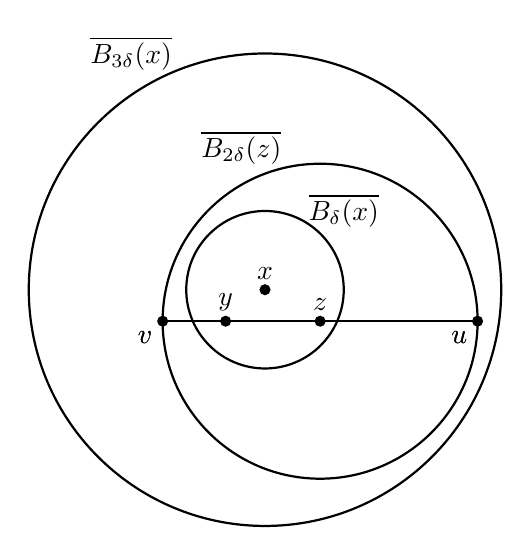
\begin{tikzpicture}[thick]
    \coordinate (u) at (-2,0);
    \coordinate (v) at (2,0);
    \coordinate (y) at (-1.2,0);
    \coordinate (z) at (0,0);

    \draw[name path={u--v}] (u) -- (v);
    \node [draw,name path=z] at (z) [circle through={(u)}] {};

    \path[name intersections={of=u--v and z,by={int_u,int_v}}]
      foreach \X in {u,v}{(int_\X) node[below left]{$\X$}};

    \fill   (int_u) circle[radius=2pt]  node [below left] {$u$};
    \fill   (int_v) circle[radius=2pt]  node [below left] {$v$};

    \fill   (z) circle[radius=0pt]  node [xshift=-1cm, yshift=2.2cm] {$\overline{B_{2\delta}(z)}$};

    \fill   (z) circle[radius=2pt]  node [above] {$z$};
    \fill   (y) circle[radius=2pt]  node [above] {$y$};

    \coordinate (x) at (-0.7,0.4);

    \draw   (x) circle[radius=1cm] node [above] {$x$};
    \fill   (x) circle[radius=2pt]  node [xshift=10mm, yshift=10mm] {$\overline{B_{\delta}(x)}$};

    \draw   (x) circle[radius=3cm] node {};
    \fill   (x) circle[radius=0pt]  node [xshift=-1.7cm, yshift=3cm] {$\overline{B_{3\delta}(x)}$};
\end{tikzpicture}
\caption{Drawing of the proof of \autoref{th:locLip}.}
\label{fig:proof_loc_lip}
\end{figure}

The main ingredient of the proof, that we mention in the proof sketch of \autoref{thmTLSlocLip}, is the following:

\begin{theorem}\label{th:locLip}
Let $f:V\subseteq (\BB R^X,\norm\cdot) \to (\BB R,\absv \cdot)$, with $V$ open and convex and $\norm\cdot$ any norm.
If $f$ is concave and locally bounded, then $f$ is locally Lipschitz.
Moreover, the Lipschitz constant of $f$ on $\overline{B_{\delta}(x)}$ can be chosen to be $\frac{1}{\delta}\max_{\overline{B_{3\delta}(x)}} \absv f$.
\end{theorem}
\begin{proof}
 Call $\overline{B_{\delta}(x)}:=B_1$, $\overline{B_{3\delta}(x)}:=B_3$.
 It suffices to show that for all $x\in V$, there is $\delta>0$ s.t.\ $B_3\subseteq \mathrm{interior}(V)$, $K:=\max_{B_3}  \absv f$ exists and $f$ is $(\frac{1}{\delta}\max_{B_3} \absv f)$-Lipschitz on $B_1$.
 A $\delta$ satisfying the first two conditions exists since $V$ is open and bcause $f$ is locally bounded and $B_3$ is compact.
 We will show that for all such $\delta$, the third condition already holds.

 For that, fix $y,z\in B_1$ and call $r:=\frac{d(y,z)}{2\delta}\in[0,1]$.
 We want to show that $\absv{f(y)-f(z)}\leq \frac{K}{\delta}d(y,z)=2Kr$.
 Wlog $y\neq z$, otherwise there is nothing to show.

 So $r\neq 0$ and we can consider $u:=\frac{1+r}{r}z-\frac{1}{r}y$, $v:=\frac{1}{r}y-\frac{r-1}{r}z$.
 We have $u,v\in \overline{B_{2\delta}(z)}=:B_2$.
 Indeed, $d(u,z)=\norm{u-z}=\norm{\frac{z}{r}+z-\frac{y}{r}-z}=\frac{\norm{z-y}}{r}=2\delta$ and similarly $d(v,z)=2\delta$.
 Geometrically, those are actually the intersections between $B_2$ and the line generated by $y$ and $z$, see \autoref{fig:proof_loc_lip}.
 Now we have the convex combinations $z=\frac{1}{1+r}y+\frac{r}{1+r}u$ and $y=(1-r)z+rv$, so the concavity of $f$ entails on one hand:
 $f(z)\geq \frac{1}{1+r}f(y)+\frac{r}{1+r}f(u)\geq \frac{f(y)}{1+r} - \frac{rK}{1+r}$, i.e.\ $f(y)-f(z)\leq r(K+f(z))\leq 2rK$, and on the other hand:
 $f(y)\geq (1-r)f(z)+rf(v)\geq f(z)-r(f(z)+K)$, i.e.\ $f(z)-f(y)\leq r(f(z)+K)\leq 2rK$.
 In the previous inequalities we have used that $f(u),f(v)\geq -K$.
 This follows because $u,v\in B_2\subseteq B_3$, as it can be immediately checked, thus $\absv{f(u)},\absv{f(v)}\leq K$.
 Putting the final inequalities together, we have $\absv{f(y)-f(z)}\leq 2rK$, i.e.\ the thesis.
\end{proof}

Therefore, since $(0,\infty)^X$ is open and convex in $(\BB R^X,\norm\cdot)$ and all tps are non-negative, we immediately have \autoref{thmTLSlocLip}.


\end{document}
